%%%%%%%%%%%%%%%%%%%%%%%%%%%%%%%%%%%%%%%%%%%%%%%%%%%%%%%%%%%%%%%%%%%%%%%%%
%                                                                       %
% ustthesis_test.tex: A template file for usage with ustthesis.cls      %
%                                                                       %
%%%%%%%%%%%%%%%%%%%%%%%%%%%%%%%%%%%%%%%%%%%%%%%%%%%%%%%%%%%%%%%%%%%%%%%%%

\documentclass[a4paper, dvipsnames]{ustthesis}
\usepackage[square,numbers]{natbib}
% \usepackage{xeCJK}
\usepackage[T1]{fontenc}
%\usepackage{algorithm}
%\usepackage{algorithmic}
% \usepackage{longtable}
% \usepackage{url}
% \usepackage{multirow}
% \usepackage{graphics}
% \usepackage{graphicx}
% \usepackage{amsmath}
% \usepackage{cases}
% \usepackage{colortbl}
% \usepackage{xcolor}
% \usepackage{times}
% \usepackage{array}
%\usepackage{hyperref}
% \usepackage{pdflscape}

% Source: https://tex.stackexchange.com/questions/45159/table-of-contents-section-titles-ragged-right
% This is for avoiding hyphenation in TOC
% \usepackage{etoolbox}
% \makeatletter
% \patchcmd{\@dottedtocline}
%   {\rightskip\@tocrmarg}
%   {\rightskip\@tocrmarg plus 4em \hyphenpenalty\@M}
%   {}{}
% \makeatother


\usepackage{fancyhdr}
\usepackage{setspace}
% \usepackage{latexsym}
    % Use the "latexsym" package when encountering the following error:
    %   ! LaTeX Error: Command \??? not provided in base LaTeX2e.
% \usepackage{epsf}
    % Use the "epsf" package for including EPS files.

%%%%%%%%%%%%%%%%%%%%%%%%%%%%%%%%%%%%%%%%%%%%%%%%%%%%%%%%%%%%%%%%%%%%%%%%%
%                                                                       %
% Preambles. DO NOT ERASE THEM. Change to suite your particular purpose.%
%                                                                       %
%%%%%%%%%%%%%%%%%%%%%%%%%%%%%%%%%%%%%%%%%%%%%%%%%%%%%%%%%%%%%%%%%%%%%%%%%

\usepackage{titlesec}


% Surrounds all chapter titles by lines (see screenshot),
% which includes the titles in the TOC and list of figures and tables
\titleformat{\chapter}[display]
{\bfseries\Huge\raggedright}
{\LARGE\chaptertitlename~\thechapter}
{2ex}
{}
[] 

% % % % The following code removes the lines (that are added above)
% % % % from the TOC and list of figures and tables
\titleformat{name=\chapter, numberless}[block]
{\centering\bfseries\huge}
{}
{0pt}
{}


% \usepackage{sectsty}
% \partfont{\centering}
% \chapterfont{\raggedright}
% \allsectionsfont{\raggedright}
% \partfont{commands}


\title{Advances in Static Analysis and Formal Verification of Smart Contracts}  % Title of the thesis.
\author{Soroush Farokhnia}     % Author of the thesis.
\degree{\PhD}             % Degree for which the thesis is. Options: \AM \MSc \MPhil \PhD
\stage{\Thesis}              % Stage of PhD document; use \Thesis for all other degree. Options: \PQE \Proposal \Thesis
\subject{Computer Science and Engineering} % Subject of the Degree.
\department{Department of Computer Science and Engineering}       % Department to which the thesis is submitted.
\advisor{Amir Kafshdar Goharshady}     % Supervisor. Additional co-supervisor can be added using \member
\member{Jiasi Shen, Thesis Supervisor}
%\acting      % Uncomment for Accting department head
\depthead{Xiaofang Zhou}     % department head.
\defencedate{2026}{01}{16}     % \defencedate{year}{month}{day}.



% Custom page numbering
% \usepackage{fancyhdr}


%%%%%%%%%%%%%%%%%%%%%%%%%%%%%%%%%%%%%%%%%%%%%%%%%%%%%%%%%%%%%%%%%%%%%%%%%
%                                                                       %
% macros.tex: Consolidated macros for PhD thesis                        %
%                                                                       %
%%%%%%%%%%%%%%%%%%%%%%%%%%%%%%%%%%%%%%%%%%%%%%%%%%%%%%%%%%%%%%%%%%%%%%%%%

%%%%%%%%%%%%%%%%%%%%%%%%%%%%%%%%%%%%%%%%%%%%%%%%%%%%%%%%%%%%%%%%%%%%%%%%%
% SHARED PACKAGES AND SETTINGS                                          %
%%%%%%%%%%%%%%%%%%%%%%%%%%%%%%%%%%%%%%%%%%%%%%%%%%%%%%%%%%%%%%%%%%%%%%%%%

% For better font rendering
% \usepackage{lmodern}
% For citations and references (adjust style as needed)
%HS: Add following for fullcite
%\usepackage[backend=biber, style=authoryear]{biblatex}
%\addbibresource{refs.bib} % Replace with your .bib file name
%\usepackage{natbib}
% make references clickable 
% \usepackage{unicode-math}
% \setmathfont{Latin Modern Math} % or another math font if you prefer

\usepackage[cal=cm,bb=ams,scr=boondoxo]{mathalfa} % One family for various math families
\usepackage{bibentry}
\usepackage[hidelinks, pdfpagelabels]{hyperref}
\usepackage{makecell}
\usepackage{rotating}
\usepackage{mathtools}
% \usepackage{amsfonts}
\usepackage{nicefrac}
\usepackage{float}
\usepackage{wrapfig}
\usepackage{amscd}
\usepackage{amsthm}
\usepackage{verbatim}
\usepackage{tikz}
\usepackage{pgfplots}
\pgfplotsset{compat=1.18}

\usetikzlibrary{calc, matrix, shapes, arrows, positioning, decorations.pathreplacing, backgrounds}
\usetikzlibrary{shapes.geometric, fit}
\usetikzlibrary{arrows.meta}
\usepackage[many]{tcolorbox}
\usepackage{color,colortbl}
\usepackage{adjustbox}
\usepackage{changepage}
\usepackage{framed}
\tikzstyle{box_nofill}=[rectangle,draw]
\tikzstyle{box_fill1}=[rectangle,draw,fill=asparagus!50,minimum size=1.4em]
\tikzstyle{box_fill2}=[rectangle,draw,fill=babyblueeyes!50,minimum size=1.4em]
% \usepackage{subcaption}
% \usepackage{pgfplots}
% \usepackage{thmtools}

% NOTE: This thesis uses the `algorithm2e` pseudocode style (\KwIn/\KwResult/\ForEach/...)
% which conflicts with the `algorithm` + `algpseudocode` combination.
% Keep only one family enabled.
%\usepackage{algorithm}
%\usepackage[noend]{algpseudocode}

\usepackage[utf8]{inputenc}
\usepackage[T1]{fontenc}
\usepackage{xspace}

\usepackage{amssymb}
\usepackage{stmaryrd}
% The stmaryrd font family doesn't provide a bold series; declare a
% substitution so LaTeX won't warn when a bold series is requested.
% If the stmaryrd FD file is available, load it first and then declare
% the bold->medium substitution for the stmry family. This avoids the
% "font family unknown" error when the FD file hasn't been read yet.
% Define the stmry math symbol font and map its bold version to the
% medium series so that bold math (e.g. via \bm) won't request a
% non-existent bold font.
\DeclareSymbolFont{stmry}{U}{stmry}{m}{n}
\SetSymbolFont{stmry}{bold}{U}{stmry}{m}{n}

% Suppress Overfull/Underfull \hbox and \vbox warnings (reduces noisy
% diagnostics in editors like VS Code). Adjust if you want looser
% control instead of fully silencing these messages.
% - \hfuzz: ignore overfull boxes smaller than this glue (in pt)
% - \hbadness: threshold for reporting underfull hbox (0..10000)
% - \vfuzz/\vbadness analogues for vertical boxes
% - \overfullrule: width of visible box in output; 0pt hides it
\hfuzz=100pt
\hbadness=10000
\vfuzz=100pt
\vbadness=10000
\overfullrule=0pt
\usepackage{etoolbox}
\usepackage{bm}
% \usepackage{cite}
%HS: Removing cite for hkust thesis template
\usepackage{textcomp}
\usepackage{tabto}
\usepackage{thm-restate}
\usepackage{blkarray}
\usepackage{refcount}

% \usepackage{lineno}
% \linenumbers

\usepackage{caption}

\usepackage{xcolor}
\def\BibTeX{{\rm B\kern-.05em{\sc i\kern-.025em b}\kern-.08em
    T\kern-.1667em\lower.7ex\hbox{E}\kern-.125emX}}


\usepackage{svg}

\usepackage[ruled,linesnumbered]{algorithm2e}

% Compatibility: some pseudocode uses \Comment{...} (algpseudocode-style) while
% the thesis otherwise uses algorithm2e keywords (\KwIn/\KwResult/\ForEach).
% Map \Comment to an algorithm2e end-of-line comment.
\providecommand{\Comment}[1]{\tcp*[f]{#1}}

\definecolor{gray}{rgb}{0.3, 0.3, 0.3}

% \SetCommentSty{\textcolor{gray}{\#}} % Gray color for comments
% \SetKwComment{tcp}{\color{gray}$\blacktriangleright$ }{}

% % Redefine comment style
% \SetCommentSty{textit} % Italicize comment
% \SetCommentSty{color{gray}} % Set color to gray
% \SetKwComment{Comment}{$\blacktriangleright$\ }{} % Use black triangle



% \usepackage{setspace}
\usepackage{listings}
\usepackage{pgf}
\usepackage{graphicx}
% \usepackage{subfig}
\usepackage{dashbox}
\usepackage{float}
\usepackage{syntax}
% \usepackage{hyperref}
\usepackage{hhline, booktabs}
\usepackage{array,multirow}	
\usepackage{tablefootnote}
% \usepackage{subcaption}
% \usepackage{longtable} % For long tables
\usepackage{cleveref}
% \usepackage{mathrsfs}
\usepackage{subcaption} 




\setlength{\fboxsep}{1pt}
\setlength{\dashlength}{4pt}
\newcommand{\codetemplate}[1]{\dbox{$#1$}}
\newcommand{\Hole}[1]{\dbox{$#1$}}
\newcommand{\errorRejected}{\textit{Failed}}
\newcommand{\errorRose}{\textit{Failed}}
\newcommand{\errorUnsat}{\textit{Unsat}}
\newcommand{\errorTimeout}{\textit{Timed out}}
\usepackage{paralist}
\usepackage{lscape}

\newcommand{\hit}[1]{\textcolor{red}{\textbf{Hitarth: }\textit{#1}}}

\usepackage{amsmath}
% \usepackage{thmtools}

\usepackage{thmtools}
\usepackage{thm-restate}


\theoremstyle{plain}
% \newtheorem{example}{Example}
% \newtheorem{definition}{Definition}
\newtheorem{namedtheorem}{Theorem}
\newtheorem{namedlemma}{Lemma}

\newtheoremstyle{noparens}% cf. p. 10 of user guide of 'amsthm' package
    {}{}{\itshape}{}%
    {\bfseries}{.}{ }%
    {\thmname{#1}\thmnumber{ #2}\thmnote{ {(\mdseries #3)}}}

\theoremstyle{noparens}
\newtheorem{theorem}[namedtheorem]{Theorem}
\newtheorem{block2024crypto}{Open problem}
\newtheorem{proposition}{Proposition}
\newtheorem{conjecture}{Conjecture}
\newtheorem*{fact*}{Fact}
\newtheorem{excont}{Example}
\newtheorem{corollary}{Corollary}
\newtheorem{lemma}{Lemma}
\newtheorem{claim}{Claim}
\newtheorem{definition}{Definition}
\newtheorem{example}{Example}
\theoremstyle{remark}
\newtheorem{remark}{Remark}
\newtheorem*{remark*}{Remark}


\renewcommand{\theexcont}{\theexample}
% \let\example\relax
% \declaretheorem[style=remark]{Example}

% CONFLICT: Multiple definitions of \paragraph exist across files
% macros-hkust.tex version (commented out):
% \renewcommand{\paragraph}[1]{\smallskip\noindent\textbf{\emph{#1}}} % Redefine paragraph to be bold and italicized
% options-macros.tex version:
% \renewcommand{\paragraph}[1]{\smallskip\noindent\textsc{{#1.}}}
% mining-ethereum-macros.tex version:
% \renewcommand{\paragraph}[1]{\smallskip\noindent\textbf{\textsc{#1.}}}
% Using mining version (bold+smallcaps) as default - CHECK THIS:
\renewcommand{\paragraph}[1]{\smallskip\noindent\textbf{\textsc{#1.}}}

\lstset
{ %Formatting for code in appendix
    numbers=left,
    stepnumber=1,
    showstringspaces=false,
    tabsize=1,
    breaklines=true,
    breakatwhitespace=false,
}


\usepackage{listings}
\definecolor{codegreen}{rgb}{0,0.6,0}
\definecolor{codegray}{rgb}{0.5,0.5,0.5}
\definecolor{codepurple}{rgb}{0.58,0,0.82}
\definecolor{backcolour}{rgb}{0.95,0.95,0.92}
\definecolor{gruen}{rgb}{0.0, 0.5, 0.0}
\definecolor{rot}{rgb}{1.0, 0.13, 0.32}

% \lstdefinestyle{C}{
% morekeywords={then}
% }

% \lstset{
%     keywords={then},
%     keywordstyle=\color{red}
% }    

\lstset{
basicstyle=\ttfamily,columns=flexible,frame=single,framerule=0pt,%
	%backgroundcolor=\color{gray!20},%
	xleftmargin=\fboxsep,%
	xrightmargin=\fboxsep,
	language=[LaTeX]TeX,%
	numbers=left,
	keywordstyle=\color{blue},%
	texcsstyle=*\color{red}\bfseries,%
	texcs={end,begin,documentclass,graphicspath},%
	mathescape=false,escapechar=|,%
	literate={<B>}{\textcolor{blue}{\string\usepackage}}1
	{\{ }{\textcolor{blue}{\{}}1
	{\}}{\textcolor{blue}{\}}}1
	{[}{\textcolor{blue}{[}}1     
	{]}{\textcolor{blue}{]}}1
        {then}{\textcolor{blue}{then }}1
}
\lstset{emph={%  
		@prog, @real, @pre, @post, @invariant, @macro, @var, @recurrence, %
	},emphstyle={\color{red}\bfseries}%
}%

% \usepackage{xcolor}


\usepackage{enumitem}
\newlist{mycompactitem}{itemize}{3} % 3 is max-depth
\setlist[mycompactitem]{leftmargin=0em,label=\textbullet, nosep}
\newlist{mycompactenum}{enumerate}{3} % 3 is max-depth
\setlist[mycompactenum]{leftmargin=.6em,label=\textnormal{(\arabic*)},nosep}

\newcommand{\aoverb}[2]{$\substack{\text{#1} \\ \text{#2}}$}


% \lstset{basicstyle=\footnotesize\ttfamily,columns=flexible,frame=single,framerule=0pt,%
% 	%backgroundcolor=\color{gray!20},%
% 	xleftmargin=\fboxsep,%
% 	xrightmargin=\fboxsep,
% 	language=[LaTeX]TeX,%
% 	numbers=left,
% 	keywordstyle=\color{blue},%
% 	texcsstyle=*\color{red}\bfseries,%
% 	texcs={end,begin,documentclass,graphicspath},%
% 	mathescape=false,escapechar=|,%
% 	literate={<B>}{\textcolor{blue}{\string\usepackage}}1
% 	{\{ }{\textcolor{blue}{\{}}1
% 	{\}}{\textcolor{blue}{\}}}1
% 	{[}{\textcolor{blue}{[}}1     
% 	{]}{\textcolor{blue}{]}}1
% }
% \lstset{emph={%  
% 		@prog, @real, @pre, @post, @invariant, @macro%
% 	},emphstyle={\color{red}\bfseries}%
% }%


\usepackage{pdfrender}
\newcommand*{\boldcheckmark}{%
	\textpdfrender{
		TextRenderingMode=FillStroke,
		LineWidth=1pt, % half of the line width is outside the normal glyph
	}{\checkmark}%
}




\lstdefinestyle{smtlib-style}
{
  language=Lisp,
  frame=single,
  % basicstyle=\ttfamily,
  keywordstyle = [1]{\color{Gray}},
  keywordstyle = [2]{\color{Blue}},
  otherkeywords = {;,<<,>>,++},
  morekeywords = [1]{;},
  keywords = [2]{define-fun, define-literal, define-let, define, declare-sort, declare-fun, LINE, (, )},
  numbers=left,
  numberstyle=\tiny,
  numbersep=5pt,
  xleftmargin=10pt,
  framexleftmargin=10pt,
  escapechar=|!,
}

\definecolor{keywordcolor}{rgb}{0.7, 0.1, 0.1}   %
\definecolor{tacticcolor}{rgb}{0.0, 0.1, 0.6}    %
\definecolor{commentcolor}{rgb}{0.4, 0.4, 0.4}   %
\definecolor{symbolcolor}{rgb}{0.0, 0.1, 0.6}    %
\definecolor{sortcolor}{rgb}{0.1, 0.5, 0.1}      %
\definecolor{attributecolor}{rgb}{0.7, 0.1, 0.1} %


\lstdefinelanguage{lean}{
  morekeywords={def,theorem,example,axiom,constant,inductive,structure,namespace,variable,universe,forall,exists},
  sensitive=true,
  morecomment=[l]{--},
  morestring=[b]{"},
  escapeinside={<@}{@>},
}

\lstdefinestyle{leanstyle}{
  language=lean,
  % basicstyle=\ttfamily,
  mathescape=true,
  commentstyle=\color{green!50!black},
  keywordstyle=\color{blue},
  stringstyle=\color{orange},
  showstringspaces=false,
  breaklines=true,
  frame=single,
  numbers=left,
  numberstyle=\tiny,
  numbersep=5pt,
  xleftmargin=10pt,
  framexleftmargin=10pt,
}



% Commands for notation

%left-right bracket 
\newcommand{\lr}[1]{\left( #1 \right)}
%letf-right curly bracket 
\newcommand{\lrcb}[1]{\left\{ #1 \right\}}

% \newcommand{\bigO}{\mathcal{O}}
\newcommand{\para}[1]{\smallskip\noindent\textbf{\mdseries\textsc{#1.}}}
\newcommand{\dom}{\textup{\textbf{dom}}}

% Additional shared macros (kept if already defined elsewhere)
\providecommand*{\serg}[1]{\textcolor{blue}{#1}}

\providecommand{\mask}{\text{m}}
\providecommand{\maxcap}{C_{\text{max}}}
\providecommand{\dptargmax}{\text{dpargmax}}

\providecommand{\econf}{E_c}
\providecommand{\edep}{E_d}
\providecommand{\valid}{\text{valid}}
\providecommand{\concat}{\circ}
\providecommand{\suff}{\text{suff}}
\providecommand{\feas}{\mathcal{F}}

% make first parameter optional:
\providecommand{\clneig}[2][]{\mathcal{N}_{#1}[#2]}

\providecommand{\tdp}{\text{tdp}}
\providecommand{\txs}{\textsf{TX}}
\providecommand{\sz}{\sigma}
\newcommand{\cfee}{\phi}


% special letters for reals, rationals, integrals 
% \newcommand{\RP}{\mathbb{R^+}}
\newcommand{\nn}{\mathbf{n}}
\newcommand{\mm}{\mathbf{m}}
\newcommand{\RR}{\mathbb{R}}
\newcommand{\QQ}{\mathbb{Q}}
\newcommand{\NN}{\mathbb{N}}
% \newcommand{\EE}{\mathbb{E}}
\newcommand{\ttt}{\mathcal{T}}
\newcommand{\ifthen}{\textcolor{blue}{\texttt{if-then}}}
\newcommand{\rex}{\mathcal{R}\texttt{-expression}}
\newcommand{\mex}{\mathcal{M}\texttt{-monomial}}
\newcommand{\QPoly}{Q\text{-Polynomial}}
\newcommand{\mtrans}{M\text{-Transformation}}

% From: https://tex.stackexchange.com/questions/323297/typing-block-matrices-with-zero-blocks-and-seperators
% \newcommand{\bigmat}[1]{\mbox{\normalfont\bfseries #1}}
% \newcommand{\rvline}{\hspace*{-\arraycolsep}\vline\hspace*{-\arraycolsep}}


\newcommand{\SAT}[1]{\textit{SAT}(#1)}
\newcommand{\monoid}{\text{monoid}}
\newcommand{\degreemath}{\textit{degree}}
\renewcommand\thmcontinues[1]{Continued}

\newcommand{\ifthenblock}[2]{\textcolor{blue}{\texttt{if}} \; (\textcolor{red}{#1}) \; \textcolor{blue}{\texttt{then}} \; \textcolor{green!50!black}{#2}}


% CONFLICT: \todo has different definitions in options-macros.tex and mining-ethereum-macros.tex
% options-macros.tex version:
% \newcommand{\todo}{\textcolor{red}{\textbf{TODO }}}
% \renewcommand{\todo}[1]{\textcolor{red}{TODO: #1}}
% mining-ethereum-macros.tex has it commented out
% Using options-macros.tex version - CHECK THIS:
\newcommand{\todo}{\textcolor{red}{\textbf{TODO }}}
% \renewcommand{\todo}[1]{\textcolor{red}{TODO: #1}}

\newcommand{\Rstep}{\underset{R}{\rightarrow}}
\newcommand{\Rstepstar}{\underset{R}{\overset{*}{\rightarrow}}} 

% for cells in the experimental section 
% \newcommand{\success}{\textcolor{green!50!black}{\textbf{+}}}
\newcommand{\fail}{\textcolor{red}{\textbf{-}}}
\newcommand{\missed}{\textcolor{blue}{\textbf{missed}}}
\newcommand{\success}{\textcolor{gruen}{\textbf{\boldcheckmark}}}
\newcommand{\unsat}{\textcolor{rot}{\textbf{UNSAT}}}
\newcommand{\tl}{\textcolor{rot}{\textbf{TL}}}
\newcommand{\wa}{\textcolor{rot}{\textbf{WA}}}
\newcommand{\ns}{\textcolor{rot}{\textbf{NS}}}
\newcommand{\unknown}{\textcolor{rot}{\textbf{NS}}}
\newcommand{\outofmem}{\textcolor{rot}{\textbf{ML}}}
\newcommand{\sat}{\textsl{SAT}}

\newcommand{\valuation}{val}
\newcommand{\val}{\valuation}
\newcommand{\vars}{\mathbb{V}}
\newcommand{\tvars}{{\mathbb{T}}}
\newcommand{\tval}{\valuation_\tvars}
\newcommand{\locs}{\mathbb{L}}
\newcommand{\loc}{\ell}
\newcommand{\transitions}{\mathcal{T}}
\newcommand{\transition}{\tau}
\newcommand{\invariant}{\mathbb{I}}
\newcommand{\cutset}{\mathcal{C}}
\newcommand{\state}{\sigma}

\newcommand{\linearexample}{\textit{VotingContract }}
\newcommand{\nonlinearexample}{\textit{NestedLoop }}


\newcommand{\qflra}{\text{QF\_LRA}\xspace}
\newcommand{\qfuf}{\text{QF\_UF}\xspace}

\newcommand{\edrat}{\textit{e}\text{DRAT}\xspace}
\newcommand{\drat}{\text{DRAT}\xspace}
\newcommand{\dimacs}{\text{DIMACS}\xspace}
\newcommand{\prop}[0]{\mathcal{P}\xspace}
\newcommand{\cvcv}{\textsc{cvc5}\xspace}
\newcommand{\tick}{\textcolor{green!50!black}{\checkmark}\xspace}
\newcommand{\noresult}{\textcolor{red!80!blue}{NA}}

\newcommand{\red}[1]{\textcolor{red!80!blue}{#1}}
\newcommand{\green}[1]{\textcolor{Green}{#1}}
\newcommand{\Gray}[1]{\textcolor{Gray}{#1}}

\newcommand{\Sat}[0]{\text{SAT}\xspace}
\newcommand{\leanvalido}[0]{\textsc{LeanValido}\xspace}
\newcommand{\valido}[0]{\textsc{Valido}\xspace}

\newcommand{\drattrim}{\texttt{DRAT-trim}}



\newcommand{\algovar}[1]{\textit{#1}}
\newcommand{\funcname}[1]{\textcolor{Blue}{\text{#1}}}
\newcommand{\toolname}[1]{\textcolor{Blue}{\text{#1}}}
\newcommand{\funcnamelean}[1]{\textcolor{Blue}{\texttt{#1}}}
\newcommand{\intextfunc}[1]{\texttt{#1}}

\newcommand{\lstcomment}[1]{\hfill \textcolor{Gray}{\textit{#1}}}


% For introduction of thesis

\tcbuselibrary{skins, breakable}

\newtcolorbox{doublebox}{
  enhanced,
  % breakable,
  colback=lightgray!10,     % light gray background
  % colframe=black,           % black border
  % boxrule=0.5pt,            % border thickness
  % frame style={double},     % double outer lines
  % sharp corners,
  % left=6pt, right=6pt, top=6pt, bottom=6pt,
}


% For nicer font for \textsc and latin quote

% \usepackage{palatino} % or mathpazo for Palatino

% Define a macro for Latin quotes in all caps
\newcommand{\latinquote}[1]{\textsc{\MakeUppercase{#1}}}

%%%%%%%%%%%%%%%%%%%%%%%%%%%%%%%%%%%%%%%%%%%%%%%%%%%%%%%%%%%%%%%%%%%%%%%%%
%                                                                       %
% OPTIONS PAPER SPECIFIC MACROS                                         %
%                                                                       %
%%%%%%%%%%%%%%%%%%%%%%%%%%%%%%%%%%%%%%%%%%%%%%%%%%%%%%%%%%%%%%%%%%%%%%%%%

\newcommand{\contract}{\mathcal{C}}
\newcommand{\wrapped}{\mathcal{W}}
\newcommand{\parties}{\mathcal{P}}
\newcommand{\party}{p}
\newcommand{\alice}{\textsc{Alice}}
\newcommand{\bob}{\textsc{Bob}}
\newcommand{\ingrid}{\textsc{Ingrid}}
\newcommand{\paul}{\textsc{Paul}}

% CONFLICT: \gamma redefined in options-macros.tex as 'gb'
% Original \gamma is a Greek letter, this redefines it - CHECK THIS:
% \renewcommand{\gamma}{gb}


%%%%%%%%%%%%%%%%%%%%%%%%%%%%%%%%%%%%%%%%%%%%%%%%%%%%%%%%%%%%%%%%%%%%%%%%%
%                                                                       %
% MINING (ETHEREUM) PAPER SPECIFIC MACROS                               %
%                                                                       %
%%%%%%%%%%%%%%%%%%%%%%%%%%%%%%%%%%%%%%%%%%%%%%%%%%%%%%%%%%%%%%%%%%%%%%%%%

% use tikz 
\usepackage{tikz,forest}

\usepackage{xparse}
\usepackage{multirow}
\usepackage{bbding} 
% \usepackage{todonotes}  % COMMENTED: conflicts with \todo command defined elsewhere

\newcommand{\ilp}[1]{\llbracket #1 \rrbracket}

% \forestset{
% default preamble={
% before typesetting nodes={
%   !r.replace by={[, coordinate, append]}
% },  
% where n children=0{
%   tier=word,
% }{  
%   %diamond, aspect=2,
% },  
% where level=0{
%   s sep'-=0.3cm,
% }{
%   if n=1{
%     edge label={node[pos=.3, above] {Y}},
%   }{  
%     edge label={node[pos=.3, above] {N}},
%   }   
% },  
% for tree={
%   edge+={thick, -Latex},
%   s sep'+=0.6cm,
%   draw,
%   thick,
%   edge path'={ (!u) -| (.parent)},
%   align=center,
% }   
% }
% }


\forestset{
default preamble={
where n children=0{
  tier=word,
}{  
  diamond, aspect=3.5,
},
where level=0{}{if n=1{
edge label={node[pos=.5, above=0.1, left] {y}},
}{  
edge label={node[pos=.5, above=0.1, right] {n}},
}
},
% for tree={
%   % edge+={thick, -Latex},
%   s sep'+=0.3cm,
%   draw,
%   thin,
%   edge path'={ (!u) - (.parent)},
%   % align=center,  
% }
}
}

% \forestset{
% default preamble={
% before typesetting nodes={
%   !r.replace by={[, coordinate, append]}
% },  
% where n children=0{
%   tier=word,
% }{  
%   %diamond, aspect=2,
% },  
% where level=0{
%   s sep'-=0.3cm,
% }{
%   if n=1{
%     edge label={node[pos=.3, above] {Y}},
%   }{  
%     edge label={node[pos=.3, above] {N}},
%   }   
% },  
% for tree={
%   edge+={thick, -Latex},
%   s sep'+=0.6cm,
%   draw,
%   thick,
%   edge path'={ (!u) -| (.parent)},
%   align=center,
% }   
% }
% }


\lstdefinelanguage{Solidity}{
	keywords=[1]{anonymous, assembly, assert, balance, break, call, callcode, case, catch, class, constant, continue, constructor, contract, debugger, default, delegatecall, delete, do, else, emit, event, experimental, export, external, false, finally, for, function, gas, if, implements, import, in, indexed, instanceof, interface, internal, is, length, library, log0, log1, log2, log3, log4, memory, modifier, new, payable, pragma, private, protected, public, pure, push, require, return, returns, revert, selfdestruct, send, solidity, storage, struct, suicide, super, switch, then, this, throw, transfer, true, try, typeof, using, value, view, while, with, addmod, ecrecover, keccak256, mulmod, ripemd160, sha256, sha3}, % generic keywords including crypto operations
	keywordstyle=[1]\color{blue}\bfseries,
	keywords=[2]{address, bool, byte, bytes, bytes1, bytes2, bytes3, bytes4, bytes5, bytes6, bytes7, bytes8, bytes9, bytes10, bytes11, bytes12, bytes13, bytes14, bytes15, bytes16, bytes17, bytes18, bytes19, bytes20, bytes21, bytes22, bytes23, bytes24, bytes25, bytes26, bytes27, bytes28, bytes29, bytes30, bytes31, bytes32, enum, int, int8, int16, int24, int32, int40, int48, int56, int64, int72, int80, int88, int96, int104, int112, int120, int128, int136, int144, int152, int160, int168, int176, int184, int192, int200, int208, int216, int224, int232, int240, int248, int256, mapping, string, uint, uint8, uint16, uint24, uint32, uint40, uint48, uint56, uint64, uint72, uint80, uint88, uint96, uint104, uint112, uint120, uint128, uint136, uint144, uint152, uint160, uint168, uint176, uint184, uint192, uint200, uint208, uint216, uint224, uint232, uint240, uint248, uint256, var, void, ether, finney, szabo, wei, days, hours, minutes, seconds, weeks, years},	% types; money and time units
	keywordstyle=[2]\color{teal}\bfseries,
	keywords=[3]{block, blockhash, coinbase, difficulty, gaslimit, number, timestamp, msg, data, gas, sender, sig, value, now, tx, gasprice, origin},	% environment variables
	keywordstyle=[3]\color{violet}\bfseries,
	identifierstyle=\color{black},
	sensitive=true,
	comment=[l]{//},
	morecomment=[s]{/*}{*/},
	commentstyle=\color{gray}\ttfamily,
	stringstyle=\color{red}\ttfamily,
	morestring=[b]',
	morestring=[b]"
}

% algo2e 
% \usepackage[ruled,vlined]{algorithm2e}  % COMMENTED: conflicts with algorithm package in shared section
% \usepackage{algorithm}
% \usepackage{algorithmic}

\newcommand{\before}{\prec}
\newcommand{\has}{\diamondsuit}
\newcommand{\atleast}{\texttt{atleast}}

\theoremstyle{plain}%
% \newtheorem{theorem}{Theorem}%  meant for continuous numbers
% \newtheorem{theorem}{Theorem}[section]% meant for sectionwise numbers
% optional argument [theorem] produces theorem numbering sequence instead of independent numbers for Proposition
% \newtheorem{proposition}[theorem]{Proposition}

% \newtheorem{proposition}{Proposition}% to get separate numbers for theorem and proposition etc.
% \newtheorem{lemma}[theorem]{Lemma}

\theoremstyle{thmstyletwo}%
% \newtheorem{example}{Example}%
% \newtheorem{remark}{Remark}%

\newtheorem{notation}[theorem]{Notation}%

% \theoremstyle{thmstylethree}%
% \newtheorem{definition}{Definition}%


% \newcommand{\fixme}[1]{{\textbf{\color{red}(fixme: #1)}}}

\newcommand{\tx}{\ensuremath{\textup{tx}}\xspace}
\newcommand{\nonce}{\ensuremath{\textup{nonce}}\xspace}
\newcommand{\addr}{\ensuremath{\textup{addr}}\xspace}
\newcommand{\hash}{\ensuremath{\textup{hash}}\xspace}
\newcommand{\txaddr}[1]{\ensuremath\tx(\text{#1})\xspace}
\newcommand{\nbhd}{\ensuremath{\textup{nbhd}}\xspace}
\newcommand{\compat}{\leftrightarrows}
\newcommand{\incompat}{\not\leftrightarrows}
\newcommand{\incompatSet}{\ensuremath{\textup{Incompat}}\xspace}
\newcommand{\feat}{\ensuremath{\textup{feat}}\xspace}
\newcommand{\resp}{\ensuremath{\textup{resp}}\xspace}
\newcommand{\subseq}{\preceq}
\newcommand{\Var}{\ensuremath{\textup{Var}}\xspace}


% % this allows to overload the \patch command to use \patch, \patch[\tx] and \patch[\tx][1]


% Command for half circle
\newcommand*\halfcirc[1][1ex]{%
  \begin{tikzpicture}
  \draw[fill] (0,0)-- (90:#1) arc (90:270:#1) -- cycle ;
  \draw (0,0) circle (#1);
  \end{tikzpicture}}

% Command for full circle
\newcommand*\fullcirc[1][1ex]{%
  \begin{tikzpicture}
  \draw[fill] (0,0) circle (#1);
  \end{tikzpicture}}

% Command for empty circle
\newcommand*\emptycirc[1][1ex]{%
  \begin{tikzpicture}
  \draw (0,0) circle (#1);
  \end{tikzpicture}}

% Just patch 
\newcommand{\mixedType}{\halfcirc[0.06]}
\NewDocumentCommand{\patch}{o o}{%
  \ensuremath{p^{\mixedType}%
  \IfValueT{#1}{_{#1\IfValueT{#2}{, #2}}}\xspace}}

% Strict patch with full circle
\newcommand{\strictType}{\fullcirc[0.06]}
\NewDocumentCommand{\patchS}{o o}{%
  \ensuremath{p^{\strictType}%
  \IfValueT{#1}{_{#1\IfValueT{#2}{, #2}}}\xspace}}

% Relaxed patch with empty circle
\newcommand{\relaxedType}{\emptycirc[0.06]}
\NewDocumentCommand{\patchR}{o o}{%
  \ensuremath{p^{\relaxedType}%
  \IfValueT{#1}{_{#1\IfValueT{#2}{, #2}}}\xspace}}

% Full set of just patches 
\NewDocumentCommand{\patchFull}{o o}{%
  \ensuremath{\textbf{P}^{\,\mixedType}%
  \IfValueT{#1}{_{#1\IfValueT{#2}{, #2}}}\xspace}}

% Strict patch with full circle
\NewDocumentCommand{\patchSFull}{o o}{%
  \ensuremath{\textbf{P}^{\,\strictType}%
  \IfValueT{#1}{_{#1\IfValueT{#2}{, #2}}}\xspace}}

% Relaxed patch with empty circle
\NewDocumentCommand{\patchRFull}{o o}{%
  \ensuremath{\textbf{P}^{\,\relaxedType}%
  \IfValueT{#1}{_{#1\IfValueT{#2}{, #2}}}\xspace}}



\newcommand\restr[2]{{% we make the whole thing an ordinary symbol
\left.\kern-\nulldelimiterspace % automatically resize the bar with \right
#1 % the function
\vphantom{\big|} % pretend it's a little taller at normal size
\right|_{#2} % this is the delimiter
}}

\newcommand{\gr}{\ensuremath{G}\xspace}

\newcommand{\patchnbhd}{\ensuremath{p}\xspace}
\newcommand{\tail}{\ensuremath{\textup{tail}}\xspace}
\newcommand{\head}{\ensuremath{\textup{head}}\xspace}
\newcommand{\core}{\ensuremath{\textup{core}}\xspace}

% for application of \forall and \exists
\newcommand{\dotapp}{\mathbf{\,.\,}}

% CONFLICT: \EE has different definitions
% macros-hkust.tex has: \newcommand{\EE}{\mathbb{E}} (commented out)
% mining-ethereum-macros.tex has: \newcommand{\EE}[1]{\mathbb{E}\left[#1\right]}
% Using mining version - CHECK THIS:
\newcommand{\EE}[1]{\mathbb{E}\left[#1\right]}
\newcommand{\EEs}[2]{\mathbb{E}_{#1}\left[#2\right]}
\newcommand{\PP}[1]{\mathbb{P}\left[#1\right]}
\newcommand{\PPs}[2]{\mathbb{P}_{#1}\left[#2\right]}

% CONFLICT: \bigO redefined
% macros-hkust.tex has: \newcommand{\bigO}{\mathcal{O}} (commented out)
% mining-ethereum-macros.tex has: \newcommand{\bigO}{\mathcal{O}}
% These are the same, using mining version - CHECK THIS:
\newcommand{\bigO}{\mathcal{O}}
\newcommand{\uniform}{\mathcal{U}}


\newcommand{\pool}{\ensuremath{{\textsf{Pool}}}\xspace}
\newcommand{\block}{\ensuremath{\textbf{\textup{block}}}\xspace}
\newcommand{\blocks}{\ensuremath{\textbf{\textup{Blocks}}}\xspace}
\newcommand{\blockopt}{\ensuremath{\textbf{\textup{block}}_{\textup{opt}}}\xspace}
\newcommand{\fee}{\ensuremath{\textup{fee}}\xspace}
\newcommand{\tip}{\ensuremath{\textup{tip}}\xspace}
\newcommand{\gas}{\ensuremath{\textsf{gas}}\xspace}
\newcommand{\feePerGas}{\ensuremath{\textup{fee/gas}}\xspace}
\newcommand{\tipPerGas}{\ensuremath{\tip/\gas}\xspace}


\newcommand{\dataset}{\ensuremath{\textup{Dataset}}\xspace}

\newcommand{\dpt}{\textup{dp}}
\newcommand{\pma}{\textup{PerfMatch}}

% CONFLICT: \RP redefined
% macros-hkust.tex has: \newcommand{\RP}{\mathbb{R^+}} (commented out)
% mining-ethereum-macros.tex has: \newcommand{\RP}{\mathcal{RP}}
% Using mining version - CHECK THIS:
\newcommand{\RP}{\mathcal{RP}}

\newcommand{\pw}{\textup{pw}}
\newcommand{\twi}{\textup{tw}}
\newcommand{\poly}{\textup{poly}}
\newcommand{\ma}{\textup{Match}}
\newcommand{\RM}{\mathcal{RM}}
\newcommand{\RI}{\mathcal{RI}}
\newcommand{\ind}{\textup{Ind}}
\newcommand{\SSt}{\textup{SStrees}}
\newcommand{\JoinN}{\textup{JoinNodes}}
\newcommand{\Schild}{\textup{SmallestChild}}

% \renewcommand{\printatom}[1]{%
% \fontsize{8pt}{10pt}\selectfont{\ensuremath{\mathsf{#1}}}}
% % reduce bond dimensions to match smaller fonts
% \setchemfig{
%   cram rectangle=false,
%   cram width=2.5pt,
%   cram dash width=0.4pt,
%   cram dash sep=1pt,
% atom sep=16pt,
%   bond offset=1pt,
%   double bond sep=2pt
% }



\newcommand{\ethsym}{%
  \!\raisebox{-0.7ex}{%
    \includegraphics[height=1.1em, trim={97 0 97 0}, clip]{figures/ethereum.pdf}%
  }%
}



% tikz block things 
% Define box dimensions as lengths
\newlength{\txBoxWidth}
\newlength{\txRowHeight}
\newlength{\txTotalHeight}
\setlength{\txBoxWidth}{0.55cm}
\setlength{\txRowHeight}{0.4cm}
\setlength{\txTotalHeight}{1.2cm}

\newcommand{\txBox}[7][.]{%
    % Parameters:
    % [#1]: border color (optional, defaults to black with '.')
    % #2: gas
    % #3: fee
    % #4: hash
    % #5: color
    % #6: column number (0-based)
    % #7: row number (0-based)
    \begin{scope}[shift={({\txBoxWidth*1.1*#6},{-\txTotalHeight*1.2*#7})}]
        % Main box with background color
        \fill[#5!15] (0,0) rectangle (\txBoxWidth,-\txTotalHeight);
        \draw[color=\ifx.#1black\else#1\fi] (0,0) rectangle (\txBoxWidth,-\txTotalHeight);
        
        % Horizontal lines for rows
        \draw[color=\ifx.#1black\else#1\fi] (0,-\txRowHeight) -- (\txBoxWidth,-\txRowHeight);
        \draw[color=\ifx.#1black\else#1\fi] (0,-2*\txRowHeight) -- (\txBoxWidth,-2*\txRowHeight);
        
        % Text content - left aligned values
        \node[anchor=west] at (-0.1,-0.5*\txRowHeight) {\scriptsize #2};
        \node[anchor=west] at (-0.1,-1.5*\txRowHeight) {\scriptsize #3};
        \node[anchor=west] at (-0.1,-2.5*\txRowHeight) {\scriptsize #4};
    \end{scope}
}
\newcommand{\txOutBoxOverlay}[4]{%
    % Parameters:
    % #1: color for the outer box
    % #2: dilation distance
    % #3: column number (0-based)
    % #4: row number (0-based)
    \begin{scope}[shift={({\txBoxWidth*1.1*#3-#2},{-\txTotalHeight*1.2*#4+#2})}]
        % Draw the overlay box with explicit width and height calculations
        \draw[color=#1, line width=1.5pt] 
            (0,0) rectangle (\txBoxWidth+2*#2,-\txTotalHeight-2*#2);
    \end{scope}
}


% Helper functions to define named coordinates for each box
\newcommand{\txDefineCorners}[2]{
    % #1: dx (column number), #2: dy (row number)
    % Upper row points (u)
    \coordinate (tx-#1-#2-ul) at (\txBoxWidth*1.1*#1, -\txTotalHeight*1.2*#2);
    \coordinate (tx-#1-#2-um) at (\txBoxWidth*1.1*#1 + 0.5*\txBoxWidth, -\txTotalHeight*1.2*#2);
    \coordinate (tx-#1-#2-ur) at (\txBoxWidth*1.1*#1 + \txBoxWidth, -\txTotalHeight*1.2*#2);
    
    % Middle row points (m)
    \coordinate (tx-#1-#2-ml) at (\txBoxWidth*1.1*#1, -\txTotalHeight*1.2*#2 - 0.5*\txTotalHeight);
    \coordinate (tx-#1-#2-mm) at (\txBoxWidth*1.1*#1 + 0.5*\txBoxWidth, -\txTotalHeight*1.2*#2 - 0.5*\txTotalHeight);
    \coordinate (tx-#1-#2-mr) at (\txBoxWidth*1.1*#1 + \txBoxWidth, -\txTotalHeight*1.2*#2 - 0.5*\txTotalHeight);
    
    % Lower row points (l)
    \coordinate (tx-#1-#2-ll) at (\txBoxWidth*1.1*#1, -\txTotalHeight*1.2*#2 - \txTotalHeight);
    \coordinate (tx-#1-#2-lm) at (\txBoxWidth*1.1*#1 + 0.5*\txBoxWidth, -\txTotalHeight*1.2*#2 - \txTotalHeight);
    \coordinate (tx-#1-#2-lr) at (\txBoxWidth*1.1*#1 + \txBoxWidth, -\txTotalHeight*1.2*#2 - \txTotalHeight);
}



% running example variavles 

\definecolor{cbUltra}{RGB}{81,81,255}      % Ultramarine Blue
\definecolor{cbMagenta}{RGB}{255,81,255}   % Magenta
\definecolor{cbCyan}{RGB}{81,255,255}      % Cyan
\definecolor{cbGreen}{RGB}{81,255,81}      % Green
\definecolor{cbYellow}{RGB}{255,255,81}    % Yellow
\definecolor{cbRed}{RGB}{255,81,81}        % Red
% disabled gray color
\definecolor{cbGrayFill}{RGB}{200,200,200}     % Gray
\definecolor{cbGrayOutline}{RGB}{230,230,230}     % Gray
% for disabled text color
\definecolor{cbGrayText}{RGB}{100,100,100}     % Gray


% Define transaction variables
\newcommand{\txheader}[2]{\txBox[white]{}{Gas $\gamma_i$}{Tip $\tau_i$}{white}{#1}{#2}}
\newcommand{\txa}[4]{\txBox{$\tx_1$}{#1}{#2}{cbUltra}{#3}{#4}}
\newcommand{\txb}[4]{\txBox{$\tx_2$}{#1}{#2}{cbMagenta}{#3}{#4}}
\newcommand{\txc}[4]{\txBox{$\tx_3$}{#1}{#2}{cbCyan}{#3}{#4}}
\newcommand{\txd}[4]{\txBox{$\tx_4$}{#1}{#2}{cbGreen}{#3}{#4}}
\newcommand{\txe}[4]{\txBox{$\tx_5$}{#1}{#2}{cbYellow}{#3}{#4}}
\newcommand{\txf}[4]{\txBox{$\tx_6$}{#1}{#2}{cbRed}{#3}{#4}}
\newcommand{\txres}[5]{\txBox[white]{$\pi_{#1}$}{$\Sigma\!\!:\,$#2}{$\Sigma\!\!:\,$#3}{white}{#4}{#5}}

% define important neighbors
\newcommand{\txaN}[4]{\txBox{$\tx_1$}{}{}{cbUltra}{#3}{#4}}
\newcommand{\txbN}[4]{\txBox{$\tx_2$}{}{}{cbMagenta}{#3}{#4}}
\newcommand{\txcN}[4]{\txBox{$\tx_3$}{}{}{cbCyan}{#3}{#4}}
\newcommand{\txdN}[4]{\txBox{$\tx_4$}{}{}{cbGreen}{#3}{#4}}
\newcommand{\txeN}[4]{\txBox{$\tx_5$}{}{}{cbYellow}{#3}{#4}}
\newcommand{\txfN}[4]{\txBox{$\tx_6$}{}{}{cbRed}{#3}{#4}}

% define off 
\newcommand{\txaOff}[4]{\txBox[cbGrayOutline]{\textcolor{gray}{$\tx_1$}}{}{}{cbGrayFill}{#3}{#4}}
\newcommand{\txbOff}[4]{\txBox[cbGrayOutline]{\textcolor{gray}{$\tx_2$}}{}{}{cbGrayFill}{#3}{#4}}
\newcommand{\txcOff}[4]{\txBox[cbGrayOutline]{\textcolor{gray}{$\tx_3$}}{}{}{cbGrayFill}{#3}{#4}}
\newcommand{\txdOff}[4]{\txBox[cbGrayOutline]{\textcolor{gray}{$\tx_4$}}{}{}{cbGrayFill}{#3}{#4}}
\newcommand{\txeOff}[4]{\txBox[cbGrayOutline]{\textcolor{gray}{$\tx_5$}}{}{}{cbGrayFill}{#3}{#4}}
\newcommand{\txfOff}[4]{\txBox[cbGrayOutline]{\textcolor{gray}{$\tx_6$}}{}{}{cbGrayFill}{#3}{#4}}



% define main transactions
\newcommand{\onDilatation}{0.4}
\newcommand{\txaOn}[4]{\txOutBoxOverlay{cbUltra}{\onDilatation}{#3}{#4}\txa{#1}{#2}{#3}{#4}}
\newcommand{\txbOn}[4]{\txOutBoxOverlay{cbMagenta}{\onDilatation}{#3}{#4}\txb{#1}{#2}{#3}{#4}}
\newcommand{\txcOn}[4]{\txOutBoxOverlay{cbCyan}{\onDilatation}{#3}{#4}\txc{#1}{#2}{#3}{#4}}
\newcommand{\txdOn}[4]{\txOutBoxOverlay{cbGreen}{\onDilatation}{#3}{#4}\txd{#1}{#2}{#3}{#4}}
\newcommand{\txeOn}[4]{\txOutBoxOverlay{cbYellow}{\onDilatation}{#3}{#4}\txe{#1}{#2}{#3}{#4}}
\newcommand{\txfOn}[4]{\txOutBoxOverlay{cbRed}{\onDilatation}{#3}{#4}\txf{#1}{#2}{#3}{#4}}

\newcommand{\expgas}{\ensuremath{\textsf{expected-gas}}\xspace}



\newif\ifisFullPaper
\isFullPaperfalse
% \isFullPapertrue

% Macro to choose between full and short versions
\newcommand{\fullOrShort}[2]{\ifisFullPaper#1\else#2\fi}



% Revision highlighting macros
% \newcommand{\added}[1]{{\textcolor{blue!80!black}{#1}}}
% \newcommand{\removed}[1]{\textcolor{red!80!black}{\sout{#1}}}


\newif\ifaddedhighlight
\addedhighlighttrue 
\ifaddedhighlight
  \newcommand{\added}[1]{{\leavevmode\color{green!40!black}#1}}
\else
  \newcommand{\added}[1]{#1}
\fi

\newif\ifremovedhighlight
\removedhighlighttrue
\ifremovedhighlight
  % \newcommand{\removed}[1]{{\leavevmode\color{red}{#1}}}
  \newcommand{\removed}[1]{}
  \else
  \newcommand{\removed}[1]{#1}
\fi


\newcommand{\mayberemoved}[1]{}

\definecolor{asparagus}{rgb}{0.53, 0.66, 0.42}
\definecolor{babyblueeyes}{rgb}{0.63, 0.79, 0.95}


\definecolor{amazonorange}{HTML}{FF9900}
% \usepackage[TS1,T1]{fontenc}
% \usepackage{fourier, heuristica}
\usepackage{array, booktabs}
%\usepackage{graphicx}
%\usepackage[x11names]{xcolor}
%\usepackage{colortbl}
\usepackage{caption}
\DeclareCaptionFont{blue}{\color{LightSteelBlue3}}

\newcommand{\foo}{\color{LightSteelBlue3}\makebox[0pt]{\textbullet}\hskip-0.5pt\vrule width 1pt\hspace{\labelsep}}

\usetikzlibrary {shapes.callouts}
\newcommand{\speechthis}[2]{
        \tikz[remember picture,baseline]{
        \node[overlay,ellipse callout,fill=blue!50, above=of #1] 
         {#2};}%
    }%


\newtcolorbox{GreenBox}[2][]{%
    enhanced,
    colback = asparagus!5!white,
    colframe = asparagus!75!black, 
    arc = 2mm, outer arc = 1mm, 
    fonttitle = \large\textbf, 
    title = #2,
    #1}

\newtcolorbox{BlueBox}[2][]{%
    enhanced,
    colback = blue!5!white,
    colframe = babyblueeyes!75!black, 
    arc = 2mm, outer arc = 1mm, 
    fonttitle = \large\textbf, 
    title = #2,
    #1}


\lstset{emph={%  
    then, if, else, while, or, invariant, int, assume, assert, and, real%
    },emphstyle={\color{red}\bfseries}%
}%

\definecolor{codegreen}{rgb}{0,0.6,0}
\definecolor{codegray}{rgb}{0.5,0.5,0.5}
\definecolor{codepurple}{rgb}{0.58,0,0.82}
\definecolor{backcolour}{rgb}{0.95,0.95,0.92}

\lstset{
    % basicstyle=\footnotesize\ttfamily,
    columns=flexible,frame=single,framerule=0pt,%
	%backgroundcolor=\color{gray!20},%
	xleftmargin=\fboxsep,%
	xrightmargin=\fboxsep,
	language=[LaTeX]TeX,%
	% numbers=left,
	keywordstyle=\color{blue},%
	texcsstyle=*\color{red}\bfseries,%
	texcs={end,begin,documentclass,graphicspath},%
	mathescape=false,escapechar=|,%
	literate={<B>}{\textcolor{blue}{\string\usepackage}}1
	{\{ }{\textcolor{blue}{\{}}1
	{\}}{\textcolor{blue}{\}}}1
	{[}{\textcolor{blue}{[}}1     
	{]}{\textcolor{blue}{]}}1
}
\lstset{emph={%  
		@prog, @real, @pre, @post, @invariant, @macro,%
        then, if, else, while, or, invariant, int, assume, assert, and, real%
	},emphstyle={\color{red}\bfseries}%
}%


\usepackage{dashbox}
\setlength{\fboxsep}{1pt}
\setlength{\dashlength}{4pt}
\usepackage{paralist}
\usepackage{lscape}


%FONT
\usepackage{lmodern}
 
% Fix: prevent hyperref warnings about `Token not allowed in a PDF string` for
% the plain-TeX font switch `\nbi` defined in `ustthesis.cls`.  Make `\nbi`
% expand to nothing when hyperref converts text to PDF strings (bookmarks,
% TOC entries, etc.).  Use AtBeginDocument so this runs after packages are
% loaded.
\AtBeginDocument{%
    \pdfstringdefDisableCommands{%
        \def\nbi{}%
    }%
}
% NOTE:
%   According to the sample shown in the guidelines, page number is
%   placed below the bottom margin.  However, if the author prefers
%   the page number to be printed above the bottom margin, please
%   activate the following command.

%\PNumberAboveBottomMargin



% Hitarth: I don't want the spacing from ustthesis.cls as I am
% manually handling it
\let\textspace\relax
\let\textspaceundo\relax

%Hitarth: 
\setcounter{tocdepth}{1}
\begin{document}
\maketitle
% \listoftables

\singlespacing
\abstract
Blockchains are a family of distributed consensus protocols that maintain a shared, append-only ledger without relying on a trusted central authority. Smart contracts are self-enforcing programs executed on blockchains. They enable applications across finance, healthcare, and supply chain management, and they secure substantial digital assets. This setting gives rise to natural optimization and verification problems, yet existing approaches often produce suboptimal results, lack strong formal guarantees, or do not scale. These limitations frequently compel developers to rely on manual audits, which are costly, error-prone, and can leave vulnerabilities undiscovered. This thesis develops theoretical and algorithmic foundations that bridge the gap between scalability and formal guarantees for smart contract analysis by capturing structural properties of contracts and their interactions through algebro-geometric methods and parameterized algorithms. These techniques advance prior work in applications including gas-cost analysis of contracts, maximizing miners' revenues, decentralized exchange routing, and compiler-level gas minimization. Beyond the core technical results, the thesis emphasizes that blockchain is inherently interdisciplinary and benefits from perspectives beyond computer science; cross-disciplinary methods can surface costly vulnerabilities that would otherwise remain undiscovered.

\endabstract
\doublespacing
\authorise

\onehalfspacing
\dedication
% This is an optional section.
\vspace{2\baselineskip}

\begin{flushright}
\textsc{To my mother,\\who always placed our education above all else.}
\end{flushright}

\vspace{2em}


\enddedication
\newpage

\acknowledgments
% Supervisors
I was privileged to have Amir Goharshady as my PhD supervisor. His insights and guidance were instrumental in my growth as a researcher. He consistently supported me in navigating career choices, grant applications, teaching opportunities, and interviews. Our long discussions about the right and wrong paths, whether in research, career, or life itself, have always been invaluable to me.
% Upon graduation, I recognize that many of these questions remain unresolved; however, his mentorship has given me the tools to pursue my own answers in the years ahead.

I am grateful to my co-supervisor, Jiasi Shen, for her consistant support throughout my time at HKUST. I also thank Prof. S. Akshay, Prof. Supratik Chakraborty, and Prof \DJ or\dj e \v{Z}ikeli\'{c} for their valuable insights that shaped my research direction and career path. My thanks extend to Prof. Dimitris Papadopoulos and Junxian He for graciously agreeing to chair my thesis defense sessions.

% Colleagues
During my PhD, I had the privilege of working alongside exceptionally talented collaborators. Sergei Novozhilov helped me navigate many complex research problems. Our stormy meetings with Harshit Motwani pushed me beyond my academic comfort zone. With Togzhan Barakbayeva, I built working solutions from our research ideas. The conversations and work we shared shaped many chapters of this thesis.


I am also grateful for the support of my ALPACAS colleagues: Jonas Ballweg, Xuran Cai, Zhuo Cai, Dr. Giovanna Kobus Conrado, Pavel Hudec, Dr. S. Hitarth, Kerim Kochekov, Chun Kit Lam, Pingjiang Li, Zhaorun Lin, Tian Shu, and Ahmed Zaher.

% Old Family
I owe a profound debt of gratitude to my parents, Marzieh Javameh and Saeid Farokhnia, for their unwavering support throughout my life. My brother Sepher also deserves equal recognition\footnote{Though I must note that fewer hours spent debating Middle-earth would likely have yielded additional papers!}.
% New Family
I must also express my deepest appreciation to my fianc\'ee, Sanaz Safaei. This doctorate would not have been possible without her kind support and encouragement. It is only fitting that our next chapter begins as this one closes.

% Teachers
I am grateful to my teachers over the years, whose guidance has brought me to this point. Mahdi Kazemi and Hossein Boomari introduced me to the world of computer science. Mohammadreza Shabanali's writings have served as my compass for personal and intellectual growth. The advice of Behnam Shakibafar and Reza Sajjadi helped me in the early stages of my career.

Finally, I am grateful to HKUST and the Ethereum Foundation, who financially supported my PhD, and to the Alexander von Humboldt Foundation, which awarded me a research fellowship.

\endacknowledgments
\newpage

\singlespacing
% Hitarth: Single spacing for TOC and Abstract
\tableofcontents
%Hitarth: Rest of the thesis in one-half spacing
\onehalfspacing

% \listoffigures


%%%%%%%%%%%%%%%%%%%%%%%%%%%%%%%%%%%%%%%%%%%%%%%%%%%%%%%%%%%%%%%%%%%%%%%%%
%                                                                       %
%     8) The Actual Contents                                            %
%                                                                       %
% The command \chapters MUST BE USED to ensure that the entire content  %
% of the Thesis is double-spaced (in version 1.0).                      %
%                                                                       %
% However, in version 2.0, \chapters will be automatically added in     %
% the beginning of the first chapter.                                   %
%                                                                       %
%%%%%%%%%%%%%%%%%%%%%%%%%%%%%%%%%%%%%%%%%%%%%%%%%%%%%%%%%%%%%%%%%%%%%%%%%

%%\chapters         % Not necessary with ustthesis.cls (v2.0).

%%%%%%%%%%%%%%%%%%%%%%%%%%%%%%%%%%%%%%%%%%%%%%%%%%%%%%%%%%%%%%%%%%%%%%%%%
%                                                                       %
% Each chapter is defined via the \chapter command. The usual sectional %
% commands of LaTeX are also available.                                 %
%                                                                       %
%%%%%%%%%%%%%%%%%%%%%%%%%%%%%%%%%%%%%%%%%%%%%%%%%%%%%%%%%%%%%%%%%%%%%%%%%

% % % Chapters

% \part*{}
% \include{chapter-conclusion/base}\label{part:i}



\chapter{Introduction}
\label{chp:intro}

\section{Prologue}

\para{Blockchain and Smart Contracts} This thesis focuses on designing automated algorithms for (i) optimization problems in blockchains and (ii) detecting vulnerabilities or mathematically verifying their absence in smart contracts. The recent success of Bitcoin~\cite{nakamoto2008bitcoin} has highlighted the potential of blockchains, encouraging researchers to extend the concept of transactions beyond the mere transfer of digital assets to the execution of arbitrary programs, known as smart contracts. Such architectures have become prevalent because centralized systems are vulnerable to fraud, censorship, and manipulation, as they depend on a single authority for control and decision-making. Thus, smart contracts, which can employ any complex logic, remove the need for intermediaries by decentralizing control, making interactions more transparent, tamper-resistant, and censorship-proof. Consequently, they have become instrumental in holding digital assets valued at billions of dollars. Currently, Ethereum, the 2nd largest cryptocurrency with a market cap of $\$354,000,000,000$, and Cardano, the 9th largest with a market cap exceeding $\$14,000,000,000$, both support the execution of arbitrarily complex smart contracts~\cite{coinmarketcap2024cryptocurrency}~\footnote{All prices and exchange rates are as of 01 January 2025.}.


\para{Motivation and Challenges} Vulnerabilities in smart contracts can have devastating consequences, making their security a critical concern. For example, the DAO attack in 2016 resulted in a loss of \$50,000,000, and a recent Bybit hack in February 2025 allowed attackers to steal more than \$1,500,000,000. These losses could have been prevented if the contracts had been formally and rigorously verified. In addition to security, there are also many unsolved or open-ended optimization problems in blockchains. A quintessential example is that users incur execution fees, known as ``gas'', when interacting with contracts. In 2024 alone, Ethereum users spent more than $\$2,700,000,000$ in gas fees. The Ethereum Foundation recognizes that these high fees present a substantial obstacle to broader adoption~\cite{farokhnia2023alleviating}. Thus, any vulnerability or inefficiency can have profound financial repercussions. Relying on unsound heuristics or suboptimal algorithms is unacceptable when billions of dollars are at stake. Rigorous, principled approaches are essential to ensure both the security and efficiency of blockchain systems.


\para{Real-World Applications of Smart Contracts} Smart contracts underpin a wide range of applications across both public and private sectors. In the public sector, they have been adopted in healthcare, crowdfunding, and supply chain management. For instance, the European Commission highlights properties such as trust, privacy, autonomy, inclusiveness, and transparency as key drivers for many projects launched to leverage decentralization for social and public good~\cite{polvora2020scanning}. Another notable example is the Bloxberg blockchain, led by the Max Planck Digital Library, which supports scientific research through smart contract infrastructure~\cite{librarynoyearfirst}. In the private sector, smart contracts have reshaped various financial services such as lending, insurance, and asset management, which are often referred to as decentralized finance (DeFi). Stablecoins like Tether (USDT) and USD Coin (USDC), with market capitalizations of $120,000,000,000$ and $50,000,000,000$, respectively, are implemented as Ethereum smart contracts~\cite{coinmarketcap2024cryptocurrency}. A further illustration is Uniswap, a decentralized exchange (DEX) that allows users to trade digital assets without intermediaries and currently secures $3,400,000,000$~\cite{labs2024uniswap}. Thus, the appeal of decentralization has drawn various professionals to blockchain. However, the cost of operations and potential vulnerabilities remain significant concerns for progress.

Given the rapid adoption of smart contracts, scalable and secure algorithms for verification and optimization are essential. Many formal methods provide soundness (and, where applicable, completeness) but do not scale, while heuristics can leave contracts vulnerable or inefficient. This thesis shows that, by exploiting structural properties of smart contracts, we can achieve the best of both worlds: principled methods that scale in practice. Building on prior work, we study two complementary approaches to these challenges.


\para{Parameterization} The first method is to utilize techniques from parameterized complexity theory.
Many optimization and verification tasks can be framed as graph problems over CFGs of programs. These problems are often intractable. When dealing with intractable problems, e.g.~NP-hard graph problems, parameterized algorithms leverage the structural and sparsity properties of the underlying graphs. Unlike traditional complexity theory, which assesses runtime based solely on input size, parameterized complexity considers both the input size and an additional property of the instance (a ``parameter''). For instance, \textit{treewidth} is a well-known parameter that measures the tree-likeness of a graph, while \textit{treedepth} formalizes the star-like structure of a graph. Many problems that are computationally intractable (e.g.~NP-hard) on general graphs can be efficiently solved on graphs with small treewidth. The intuition is that, if a graph can be decomposed into small parts that are connected to each other in a tree-like manner, then one can treat the graph as if it were a tree and leverage tree-based algorithmic ideas such as bottom-up dynamic programming. It is well known that CFGs of structured programs are sparse and tree-like, i.e.~they have bounded treewidth~\cite{thorup1998all}. The same has also been established for smart contracts~\cite{chatterjee2019treewidth}. See Section~\ref{sec:prelim-parameters} for more details.

\para{Algebro-geometric Methods} Our second approach uses tools from polyhedral and real algebraic geometry. Many of our problems can be formulated as solving systems of constraints. If we submit these constraints directly to a Non-linear Real Arithmetic (NRA) or SMT solver, the solver must handle quantifier alternation, which is very costly. In practice, first-order theories of the reals are slow and often fail even on small examples. To address this, we eliminate quantifier alternation by converting the original formula into an equivalent system of constraints. This produces a quantifier-free instance that is much easier for solvers to process. See Section~\ref{sec:prelim-positivity} for more details.

    
\section{Outline}
This thesis is organized as follows. Chapter~\ref{chp:prelim} presents background on blockchains and smart contracts common to most systems. It then gives system-specific details for Bitcoin (Section~\ref{sec:prelim-bitcoin}), Cardano (Section~\ref{sec:prelim-cardano}), and Ethereum (Section~\ref{sec:prelim-ethereum}). The chapter also introduces the formal definitions and mathematical tools used throughout the thesis, covering parameterized complexity in Section~\ref{sec:prelim-parameters} and algebraic and geometric methods in Section~\ref{sec:prelim-positivity}.

The main body develops principled, scalable methods for two complementary classes of problems: (i) program-level analysis of smart contracts (Chapters~\ref{chp:asparagus} and~\ref{chp:superopt}); and (ii) interactions between users and contracts (Chapters~\ref{chp:mining} and~\ref{chp:hermes}). Chapter~\ref{chp:options} further illustrates that blockchain is inherently interdisciplinary and that rigorous analysis benefits from perspectives beyond computer science. While not the main focus, this demonstrates that mathematically grounded, cross-disciplinary methods can yield novel insights. Each technical chapter presents a clear problem statement, algorithms, and empirical evaluation.

Concretely, the thesis contains the following chapters:

\begin{itemize}
    \item Chapter~\ref{chp:asparagus} proposes a novel approach to automatically synthesize parametric gas-usage upper bounds for smart contracts, using tools and theorems from polyhedral and real algebraic geometry. To the best of our knowledge, this is the first identified use case of algebro-geometric methods in blockchain. Moreover, our approach is the first to successfully synthesize polynomial bounds.

    \item Chapter~\ref{chp:superopt} studies the compiler-optimization problem of gas minimization. We present a dynamic-programming algorithm that builds on, and integrates with, the existing tool \texttt{syrup}, producing more gas-efficient bytecode while retaining correctness guarantees.

    \item Chapter~\ref{chp:mining} addresses block-construction and transaction-selection problems from a miner's perspective for two major cryptocurrencies:
    
    \begin{itemize}
        \item for Cardano (UTXO-based), we present a novel algorithm that exploits the sparsity of interrelations between Cardano transactions. We formulate this problem as a knapsack problem and derive an exact parameterized algorithm based on treewidth;
        
        \item for Ethereum (account-based), we present a novel randomized approach to boost miners' transaction-fee revenues. We observe that a transaction's gas usage is often influenced by a small subset of other transactions, termed its neighborhood.
        Our algorithm uses testing and decision trees to estimate neighborhoods, then derives gas-usage rules to predict each transaction’s fee. The rules are encoded as an ILP instance and solved with an external ILP solver.
    \end{itemize}

    \item Chapter~\ref{chp:hermes} presents an extension of a treewidth-based algorithm for optimal routing on DEXs. By leveraging the structural properties of liquidity pools, the proposed approach bridges the gap between scalability and robustness. To our knowledge, this is the first application of parameterized algorithms in the context of DEXs.
    
    \item Chapter~\ref{chp:options} refutes several common misconceptions regarding Bitcoin's security against block-reverting attacks. Specifically, we show that a successful block-reverting attack does not necessarily require (even close to) a majority of the hash power, and that Bitcoin derivatives, i.e.~options and futures, imperil Bitcoin's security by creating an incentive for a block-reverting/majority attack.
\end{itemize}


Finally, Chapter~\ref{chp:conclusion} provides a discussion of broader impacts and summarizes the main findings and future directions of the thesis.


\section{Summary of Contributions}
The main contributions of each chapter are outlined below:

\begin{itemize}
    \item In Chapter~\ref{chp:asparagus}, we consider the problem of finding polynomial gas-usage upper bounds for every function of a given smart contract. We model smart contracts as polynomial transition systems (PTSs), and our contributions are as follows:
    \begin{itemize}
        \item \emph{Theoretical Contributions.} We provide novel and fully automated algorithms, based on techniques from polyhedral and real algebraic geometry, to synthesize the tightest possible polynomial gas upper bounds for a given PTS. We show that our approach is not only sound, but also semi-complete, i.e.~complete when the polynomial degree is sufficiently large. Our theoretical approach is language-independent and can be applied to smart contracts written in any language and run on top of any blockchain protocol.
        \item \emph{Practical Contributions.} We provide extensive experimental results on 156,735 functions from 24,188 real-world smart contracts, showing that our approach is scalable and applicable to the vast majority of real-world Ethereum contracts (80.56\%). Moreover, we compare our results with GASTAP, the only previous method that could synthesize parametric bounds. Our experiments demonstrate that Asparagus outperforms GASTAP both in terms of the number of contracts it can handle and the quality and tightness of the bounds.
    \end{itemize}

    \item In Chapter~\ref{chp:superopt}, we study the compiler-optimization problem of gas minimization, and we make the following contributions:
    \begin{itemize}
        \item \emph{Theoretical Contributions.} We provide a simple dynamic-programming approach to enhance superoptimization techniques for reducing the gas usage of smart contracts.
        \item \emph{Practical Contributions.} We implement our approach and integrate it with \texttt{syrup 2.0}, the current state-of-the-art gas optimizer for Ethereum smart contracts. Over a benchmark set of \todo{148} real-world and commonly called smart contracts on the Ethereum blockchain, we find that our approach more than doubles the benefits of \texttt{syrup}, increasing gas savings from \todo{4.17}\% to \todo{11.23}\%.
    \end{itemize}

    \item In Chapter~\ref{chp:mining}, we consider the problem of Maximizing miner/producers revenues, i.e.~a block with maximum total transaction fees, in Cardano and Ethereum. Our contributions are as follows:
    \begin{itemize}
        \item For Cardano, we exploit the sparsity of interrelations between real-world Cardano transactions to find the optimal block to mine. Specifically:
        \begin{itemize}
            \item \emph{Theoretical Contributions.} Since the problem is NP-hard, we obtain an algorithm that has polynomial runtime for real-world instances of the problem. Formally, we consider a graph of interrelations between transactions and show that when this graph has bounded treedepth, i.e.~when it is sparse and resembles a shallow tree, there is a polynomial-time algorithm for finding the optimal block to mine.
            
            \item \emph{Practical Contributions.} We experimentally show that the small-treedepth assumption holds for real-world Cardano instances. With the help of the Cardano Foundation, we conduct a \todo{50}-day-long experiment on the Cardano blockchain in which we run our algorithm on the same sets of transactions as those available to real-world Cardano block producers and compare the blocks produced by our approach with those actually added to Cardano. Our approach increases transaction-fee revenues by \todo{1,357.82} USD/day (= \todo{495,604.3} USD/year). Thus, producing optimal blocks that maximize transaction fees yields significant benefits in practice.
        \end{itemize}

        \item For Ethereum, we design and present a randomized algorithm to create a block that maximizes the miner's total tip revenue. Specifically:
        \begin{itemize}
            \item \emph{Theoretical Contributions.} We execute test cases (random permutations of transactions in a transaction pool) and profile their gas usage. Then, using decision trees, for every transaction in the pool, we identify a set of other transactions that can affect its gas usage; we call this set its \emph{neighborhood}. Intuitively, we expect neighborhoods to be small because most transactions are independent; for example, two transactions that do not access the same smart contracts cannot affect each other's gas usage. We provide a probabilistic argument showing that, with high probability, our testing covers every possible permutation of each neighborhood. We cut, mix, and glue together parts of our test cases to create a block that maximizes the miner's total tip revenue. We model this step as an ILP instance and solve it using an external optimization suite. All steps of our algorithm are parallelizable and, except for the ILP solver, run in polynomial time. Because it relies on randomized sampling and ILP solvers, our algorithm is not guaranteed to always produce an optimal result.
            
            \item \emph{Practical Contributions.} We implement our algorithm and perform extensive experiments on 50,000 Ethereum blocks. For each block, we gather real-world transaction pool data and execute our algorithm. We then compare the tip revenues obtained by our framework with those of real-world miners. Our approach increases tip revenues by 73.45\% on average per block, corresponding to roughly 24.1 USD per block and 63,357,892 USD per year at current exchange rates. We also compare our tool against the default Ethereum implementation and find that our approach increases tip revenues by 18.56\% on average per block, corresponding to roughly 17.3 USD per block and 45,416,764 USD per year.
        \end{itemize}
    \end{itemize}
    
    \item In Chapter~\ref{chp:hermes}, we analyze the structural properties of Uniswap exchange pools, with the following contributions:
    \begin{itemize}
        \item \emph{Theoretical Contributions.} We extend a parameterized algorithm that leverages the low treewidth of DEX graphs to find routes efficiently. The algorithm is specifically tailored for the dynamic, online environment of DEXs, where liquidity pools are constantly changing. Our formal complexity analysis shows that its theoretical runtime outperforms state-of-the-art algorithms.
        \item \emph{Practical Contributions.} We implement the algorithm in an open-source routing tool called Hermes and conduct a comprehensive experimental evaluation using real-world Uniswap transaction data covering \todo{$20{,}000$} blocks. The results show that our treewidth-based approach achieves superior practical performance compared to existing methods. Hermes is the only method capable of processing token sets of size $100{,}000$, with an average query time of 0.19 seconds. For instances where both tools yield results, Hermes reduces the average runtime from 2.81 seconds to 0.0002 seconds, an improvement of over four orders of magnitude.
    \end{itemize}

    \item In Chapter~\ref{chp:options}, we refute several common misconceptions regarding Bitcoin's security against block-reverting attacks. In particular, we show that:
    \begin{itemize}
        \item a successful block-reverting attack does not necessarily require (even close to) a majority of the hash power;
        \item obtaining a majority of the hash power (or a sufficient minority for a block-reverting attack) costs roughly 6.77 billion USD or 2.90 billion USD, respectively, which is far lower than commonly assumed and about two orders of magnitude smaller than the Bitcoin market cap; and
        \item Bitcoin derivatives (options and futures) can imperil Bitcoin's security by creating incentives for block-reverting/majority attacks.
    \end{itemize}
\end{itemize}

\section{Awards}
The research presented in Chapter~\ref{chp:mining} received an Academic Grant (ESP) from the Ethereum Foundation. Chapter~\ref{chp:superopt} led to the award of a research fellowship from the Humboldt Foundation. The work on Cardano block production (Sections~\ref{sec:mining-cardano-problem}--\ref{sec:mining-cardano-experiments}) was conducted in collaboration with the Cardano Foundation, and the resulting research was invited for presentation at the Cardano Summit~2024.
Chapters~\ref{chp:mining} and~\ref{chp:asparagus} each received a Research Travel Grant from the Hong Kong Research Grants Council to attend the conference and present the paper.
\newpage

\chapter{Preliminaries}
\label{chp:prelim}



\section{Blockchain and Smart Contracts} \label{sec:prelim-blockchain}
\paragraph{Blockchain} As pioneered by Bitcoin~\cite{nakamoto2008bitcoin}, most modern cryptocurrencies use a blockchain protocol. There are three fundamental objects: transactions, blocks, and the blockchain. Transactions are the basic units of record keeping, defining the cryptocurrency's history and order. In Bitcoin, transactions transfer money in the underlying cryptocurrency. Anyone can create and broadcast transactions, which must be validated, e.g.~by checking digital signatures to prove ownership. Valid transactions are spread across the network using a peer-to-peer gossip protocol. Valid transactions are grouped into blocks of fixed maximum size, and each block contains a hash pointer to the previous block, forming a singly-linked list called the blockchain. Each node maintains a local copy of the blockchain, so its history consists of all transactions in its chain, which also provides their ordering.



\paragraph{Consensus mechanism} To ensure consensus, not every propagated transaction is finalized immediately; a consensus mechanism is required to make all nodes eventually agree on the blockchain's contents. Its purpose is to make adding new blocks subject to rules that prevent attackers from creating competing branches, or forks, which represent incompatible transaction histories. There are many consensus protocols~\cite{xu2023survey, dziembowski2015proofs, chatterjee2019hybrid, ball2017proofs, yin2019hotstuff}, with the most prominent being proof of work, used by Bitcoin~\cite{nakamoto2008bitcoin} and Ethereum Classic, and proof of stake~\cite{king2012ppcoin, kiayias2017ouroboros}, used by Ethereum~\cite{wood2014ethereum}, Cardano~\cite{david2018ouroboros}, and Algorand~\cite{chen2019algorand1}. In practice, different terms are used for miners; for example, Ethereum and most proof-of-stake currencies use \emph{validators} or \emph{block builders} to indicate they do not use proof of work. In this thesis, we use the term \emph{miner} for all consensus mechanisms.

\paragraph{Mining} Every blockchain protocol requires a process to extend the chain by adding new blocks. This process is often called \emph{mining} in proof-of-work blockchains such as Bitcoin~\cite{nakamoto2008bitcoin} and entails finding a solution to a proof-of-work puzzle which is often based on inverting hash functions. While proof-of-stake blockchains~\cite{king2012ppcoin, kiayias2017ouroboros} and other alternative consensus mechanisms such as proof-of-space~\cite{park2018spacemint} do not require the expensive step of solving a hash puzzle, they nevertheless need rules for extending the chain. The nodes that take part in chain extension are known by various names such as validators, farmers or producers. For simplicity, in this thesis, we simply use the words \emph{miner} and \emph{producer} to refer to any node on the network who tries to add a new block to the blockchain according to the underlying consensus protocol. 

\paragraph{Mining Steps} A miner has to first form a block by choosing a set of unmined transactions. Following Bitcoin~\cite{nakamoto2008bitcoin}, most blockchain protocols have a maximum size limit on the blocks, thus the miner has to strategically pick the transactions that are included in her block. The miner then proposes the block by publicly announcing it. The proposed block may or may not be adopted by the network, based on its rules of consensus. For example, in a proof-of-work cryptocurrency, only blocks that contain a valid solution to the hash puzzle may be accepted by the network.

\paragraph{Transaction Fees} Given that consensus heavily relies on miners and that mining is often costly, especially in proof-of-work settings, the protocol must provide rewards to incentivize mining. The miners are paid a fixed reward for every block they add to the blockchain. This is also how new units of currency are created. Additionally, to incentivize the miners to create non-empty blocks, a user who creates a transaction can decide on a transaction fee, which will be paid to the miner who adds it to the blockchain. It is well-known in the community that transactions with low fees are often ignored by the miners.

\paragraph{Smart Contracts} 
Bitcoin supports a limited scripting language for specifying conditions to spend a UTXO, such as requiring multiple signatures. In contrast, programmable blockchains, pioneered by Ethereum~\cite{wood2014ethereum}, allow arbitrary scripts in a Turing-complete language. The key idea is that blockchain consensus is independent of transaction type, enabling transactions beyond simple currency transfers. On Ethereum, a transaction can: (i)~transfer money, (ii)~deploy a \emph{smart contract}—a program in Ethereum Virtual Machine (EVM) bytecode, or (iii)~interact with existing smart contracts by calling their functions. A smart contract is a program added to the blockchain, making its code immutable. Each contract has dedicated storage and can hold currency. Once money is sent to a contract, it can only be recovered if the contract’s code transfers it elsewhere. Since the protocol provides consensus on transaction history, it also extends to the state of every contract, as all nodes can execute the transactions.

\paragraph{Design Choices in Blockchains} While blockchains share fundamental principles, their differences, such as programming language and execution environment, can influence tasks such as smart contract optimization. Blockchains typically employ either imperative or functional programming languages. Imperative languages, such as Solidity used by Ethereum, execute instructions sequentially, while functional languages, like Plutus on Cardano, rely on nested function calls. Imperative languages offer straightforward control flow and are familiar to most developers, making them easier to learn and use for a wide range of applications. In contrast, functional languages emphasize immutability and stateless computation, which can enhance security and facilitate formal verification. In terms of execution environment, Ethereum adopts an account-based model with a global state, enabling complex contract interactions, whereas Cardano uses a UTXO-based model with local state, facilitating better parallelization~\cite{wood2014ethereum,foundationnoyearplutus}.

We next review Bitcoin, Cardano, and Ethereum, emphasizing aspects relevant to this thesis.


\section{Bitcoin Architecture}
\label{sec:prelim-bitcoin}

\paragraph{Bitcoin} Bitcoin~\cite{nakamoto2008bitcoin} was the first working protocol for a decentralized cryptocurrency and currently holds the largest market cap among all such currencies, 
amounting to more than 1.4 trillion USD at the time of writing~\cite{coinmarketcap2024cryptocurrency}\footnote{The time of writing is April 1st, 2024.}. 
There is also a huge derivatives market on Bitcoin with trade volumes that often exceed 1 trillion USD per calendar month and have recently even exceeded 2 trillion USD per month (Section~\ref{sec:options-future}).

\begin{figure}[H]
	\centering
	\includegraphics[width=0.7\linewidth]{chapters/options/bitcoin.pdf}
	\caption{A simplified view of the blockchain}
	\label{fig:options-bitcoin}
\end{figure} 

\paragraph{Proof-of-Work~\cite{nakamoto2008bitcoin, gervais2016security}} In Bitcoin, transactions are grouped into \emph{blocks} of a fixed maximum size. The blocks are then chained together in a singly-linked list using hash pointers with each block containing the hash of its parent (previous) block. This linked list is aptly named the \emph{blockchain}. The blockchain is subject to consensus, i.e.~all honest nodes on the network should eventually agree on its contents. Thus, adding a new block to the end of the blockchain is a deliberately hard task, called \emph{mining}, that requires the solution of a computationally-intensive hash inversion puzzle. This scheme is called \emph{proof-of-work} and ensures that a miner's chance of adding the next block to the blockchain is proportional to the miner's computational power, i.e.~how many hashes she can compute per unit of time.

Figure~\ref{fig:options-bitcoin} shows an overview of this process. In this figure we have omitted implementation details that are not relevant to this thesis. Each block $B_i$ contains the hash of the previous block $B_{i-1}.$ This serves as a hash pointer in the linked list. It also contains a nonce $n_i$ and a sequence of transactions $Tx_{i,1}, Tx_{i,2}, \ldots.$ A miner who aims to add a new block $B_{i+1}$ should first create the pointer to the previous block and populate a list of transactions that she intends to include. She should then choose the new nonce $n_{i+1}$ such that the hash $h(B_{i+1})$ of her new block is below a certain predefined threshold\footnote{In Bitcoin, the threshold changes dynamically to ensure that a new block is mined roughly every 10 minutes.}. Since the output of a hash function is unpredictable and an ideal cryptographic hash function can be modeled as a random oracle, the miner's only choice is to repeatedly try different nonces until she finds a valid block. Thus, her success probability is proportional to the number of hashes she can compute per unit of time.

Since mining is an expensive activity, due to both hardware and electricity costs, the miner should be financially incentivized to perform it. Bitcoin creates two incentives for the miner~\cite{meybodi2022optimal, nakamoto2008bitcoin, barakbayeva2024blockchain}: (a)~a block reward (currently 6.25 BTC $\approx$ 445,835 USD, expected to halve in almost three weeks from now) is paid to each miner who successfully adds a new block, and (b)~each transaction contains a transaction fee that is paid to the miner who adds it to the consensus chain.

\paragraph{UTXO} In Bitcoin~\cite{nakamoto2008bitcoin}, each transaction has multiple inputs and outputs: inputs are coins entering the transaction, outputs are coins leaving. Each input must reference an output from a previous transaction, ensuring only previously received coins can be spent. To prevent double-spending, each output can be spent only once. Spendable coins are called Unspent Transaction Outputs (UTXOs). Although UTXOs can be reconstructed from history, Bitcoin nodes maintain a current UTXO set for efficient transaction and block validation. Since transactions cannot create new coins, the sum of outputs must be less than the sum of inputs; the difference is paid to the miner as a transaction fee. Thus, each transaction has a fixed, known fee independent of other transactions. 

% \paragraph{Architecture (Nodes, Mempool, and Block Structure)} TODO: Full nodes, mempool, block header/tx list, Merkle root, propagation constraints.
% \paragraph{Bitcoin Scripting Language} TODO: Script as spending predicate language (stack-based, restricted); mention typical policies (multisig/timelock).

\paragraph{Longest Chain Rule~\cite{nakamoto2008bitcoin, blum2020combinatorics}} In the event that two miners find a valid block at approximately the same time, a temporary \emph{fork} happens in which there are two valid blockchains known to the network. In such a scenario, the Bitcoin protocol allows miners to try to extend either branch. However, as soon as a branch becomes longer than the other(s), the shorter branch(es) are dropped by everyone who honestly follows the protocol. Thus, the protocol mandates that the longest chain is always the consensus chain and that every node on the network must always consider the longest chain known to them as the authoritative blockchain\footnote{In practice, the length of a chain is not just the number of blocks in it, but rather the total difficulty of mining these blocks. However, this minor detail does not change any of the analyses in this thesis.}. This is illustrated in Figure~\ref{fig:options-longest}. As long as a majority of the computational power on the network follows the protocol honestly, all honest participants are guaranteed to eventually reach a consensus about the blockchain.

\begin{figure}
	\center
	\includegraphics[width=0.8\linewidth]{chapters/options/longest.pdf}
	\caption{An illustration of the longest chain rule in Bitcoin}
	\label{fig:options-longest}
\end{figure}

\paragraph{Double-Spending~\cite{rosenfeld2014analysis, nakamoto2008bitcoin, karame2012double, chaudhary2020double, karame2015misbehavior}} Preventing double-spending is arguably the main contribution of the Bitcoin protocol. A \emph{double-spending} attack is when a Bitcoin user tries to use the same coin (transaction output) in two different transactions. In such cases, the two transactions will be in conflict~\cite{meybodi2022optimal} and at most one of them can be added to the consensus chain. Specifically, if $Tx_1$ and $Tx_2$ both spend the same coin, then any proposed block that contains $Tx_1$ can only be valid if neither it nor any of its ancestors (previous blocks) contain $Tx_2.$
Suppose $\alice$ is selling an item to $\bob$ and $\bob$ is paying the price by a Bitcoin transaction $Tx_1$ that transfers part of his money to $\alice$. In this case, it is not enough for $\alice$ to see $Tx_1,$ since $\bob$ might have created a conflicting transaction $Tx_2$ that double-spends the same coin. Thus, $\alice$ should wait for $Tx_1$ to be added to the consensus chain. However, even this does not guarantee that the payment is finalized, since it is possible that the miner eventually creates a longer chain that contains $Tx_2$ and thus consensus switches from $Tx_1$ to $Tx_2.$ In such cases, we would say that $Tx_1$ is \emph{reverted}. In practice, this is unlikely to happen if $Tx_1$ is already in a block $B_i$ and there are many blocks added after $B_i.$ Such blocks are called \emph{confirmation} blocks. The conventional wisdom and industrial standard practice is to wait for 6 confirmations before considering the transaction as irreversible, although some users take the risk of waiting for fewer confirmations~\cite{hou2020study}.
% TODO add a short sentence about majority attack

\section{Cardano Architecture}
\label{sec:prelim-cardano}

\para{Cardano~\cite{hoskinson2017why}} Cardano is an open and decentralized blockchain platform that supports many cryptocurrencies and tokens. Its main currency, Ada, is currently one of the top 10 cryptocurrencies in terms of market cap and has a value of more than 16 billion USD~\cite{coinmarketcap2024cryptocurrency1}. Similar to Bitcoin, Cardano follows the (extended) UTXO model~\cite{foundation2017eutxo}, in which every transaction has a set of inputs and outputs. Each input to a transaction should be an output of a previous transaction and no output may be spent (used as input) twice. It has two major advantages over Bitcoin: (i)~support for arbitrarily complex smart contracts, i.e.~transactions can invoke executions of programs in an expressive programming language, and (ii)~a proof-of-stake consensus protocol, namely Ouroboros Praos~\cite{david2018ouroboros}, which avoids the costly mining process of Bitcoin's proof-of-work. In this section, we consider a simplified model of a Cardano transaction that precisely captures those aspects which are important to this thesis. For a more thorough treatment, see~\cite{hoskinson2017why} or~\cite{brunjes2020utxo}.

\para{EUTXO} Most modern blockchains either follow the Unspent Transaction Output (UTXO) model, as in Bitcoin~\cite{nakamoto2008bitcoin}, or the account model, as in Ethereum~\cite{wood2014ethereum}. To take advantage of the benefits of both models, Cardano proposes the Extended~UTXO (EUTXO) model that allows having more expressive programs than simple scripts without adopting the account model. In UTXO, a transaction has a set of inputs and outputs. An input points to an output of a prior transaction that provides funds to be spent by this transaction. Moreover, every output can be used by at most one input. EUTXO follows the same policies except that there is one more output field called ``datum'' that carries contract-specific data. In addition, EUTXO allows the inclusion of arbitrary logic as scripts and the use of the data fields to decide if the transaction output can be spent. See~\cite{foundation2017eutxo, brunjes2020utxo} for a more detailed treatment. 

% \para{Smart Contracts and Scripting} TODO: Explain validator scripts, datum/redeemer/context; mention Plutus~\cite{foundationnoyearplutus}.

\para{Proof-of-Stake~\cite{documentation2024proof, king2012ppcoin, kiayias2017ouroboros}} In proof-of-stake protocols, a miner is randomly chosen to add the next block. Each miner's probability of being chosen is proportional to her stake in the currency, i.e.~the number of coins she holds. Specifically, in Cardano's implementation of Ouroboros Praos~\cite{david2018ouroboros}, time is divided into epochs, each consisting of 432,000 slots. Each slot corresponds to one second. Thus, each epoch lasts for five days. In each slot, some miners/producers are randomly selected to propose blocks of transactions~\cite{documentation2024slots}.  

\para{Stake Pools and Delegation~\cite{documentation2024stake}} Any user who holds Ada can take part in mining (block production) on Cardano. Users can also delegate their mining rights (stakes) to others, leading to stake pools which, as the name suggests, pool together stakes from many different users. The pool operator can then mine on behalf of all of its users and the probability that the pool is selected in each slot is proportional to the total stake of the members. The vast majority of Cardano blocks are produced by stake pools rather than individual stakeholders. 

\para{Rewards} Producing blocks is a costly process. This is of course evident in proof-of-work blockchains, in which the miners have to solve hash puzzles requiring vast computational resources and electricity usage. Thus, Bitcoin rewards miners for every new block that they successfully add to the blockchain and also pays them transaction fees~\cite{nakamoto2008bitcoin}. Even in proof-of-stake blockchains, there are costs associated with block production, e.g.~the miner has to keep track of the whole history of the chain, constantly listen for new transactions, hold stake or convince others to delegate stakes to her, form valid blocks of transactions and announce/propose them on time. Therefore, it is necessary to incentivize block production by rewarding the miners. In Cardano, the block producers are rewarded in two ways~\cite{documentation2024pledging}:
\begin{enumerate}
	\item \emph{Transaction Fees:} Every transaction contains a fixed fee. After each epoch, the fees of all transactions mined in that epoch are divided among the block producers.
	\item \emph{Monetary Expansion:} For each epoch, a fixed percentage of the remaining reserve of Ada is paid to all block producers of the epoch. 
\end{enumerate}

\para{Block Constraints} 
In Cardano's EUTXO model, a block contains a sequence of valid transactions. The transactions in each block must satisfy the following requirements, otherwise the block is considered invalid and will be discarded by all nodes of the network. 

\begin{itemize}
\item \textit{Transaction Dependencies.}
If a transaction $t_2$ uses an output of another transaction $t_1$ as one of its inputs, then $t_2$ depends on $t_1.$ If the block producer decides to include $t_2$ in her new block, then she must also add $t_1$ in the same block and before $t_2$. See Figure~\ref{fig:prelim-cardano-dep} as an example.

\begin{figure}[H]
	\centering
	\includegraphics[scale=0.75]{chapters/mining/mining-cardano-figures/dependency.pdf}
	\caption{Alice pays 15 Ada to Bob in $t_1$. In $t_2$ Bob uses the same funds to pay 10 Ada to Carol and 5 Ada back to himself. The transaction $t_2$ has an input that is using an output of $t_1.$ Thus, $t_1$ is a dependency of $t_2.$}
	\label{fig:prelim-cardano-dep}
\end{figure}

\item \textit{Transaction Conflicts.} 
If two transactions $t_2$ and $t_3$ both spend the same output of a transaction $t_1$, since every output may be spent at most once, only one of the conflicting transactions may be selected and included in the new block. Thus, the block producer has a choice to include $t_2, t_3$ or neither in the new block, but she cannot include both. See Figure~\ref{fig:prelim-cardano-conf} as an example.

\begin{figure}
	\centering
	\includegraphics[scale=0.6]{chapters/mining/mining-cardano-figures/conflict.pdf}
	\caption{In an auction contract, Alice has bid 5 Ada in $t_1$. Both Bob and Carol are trying to bid right after Alice, hence using $t_1$'s datum output as input to their transactions $t_2$ and $t_3$. Since every output can be used only once, $t_2$ and $t_3$ are in conflict.}
	\label{fig:prelim-cardano-conf}
\end{figure}
 

\item \textit{Block Size Limit.}
Cardano imposes a block size limit, i.e.~the total size of all transactions included in a new block must not exceed 90112 bytes = 88 kilobytes. This is to ensure that the blocks are small enough to be efficiently propagated within the network with minimal latency. The block size limit may change in each epoch, but in practice it has been consistently kept at 88 kilobytes.
\end{itemize}



\section{Ethereum Architecture}
\label{sec:prelim-ethereum}

This section provides a quick introduction to Ethereum and its gas model, following~\cite{wood2014ethereum, dameron2019beige}.

% \para{Architecture (Execution and Consensus)} TODO: Execution layer (EVM/world state) vs consensus layer; mempool; (optional) PBS/MEV context.
% \para{Consensus Model (Proof-of-Stake)} TODO: Validator roles, fork choice vs finality, and reorg/finality intuition (e.g.~\cite{zhang2025available}).

\para{Smart Contracts} Ethereum~\cite{wood2014ethereum} allows arbitrary programs written in a Turing-complete language, which are called \emph{Smart contracts}. Most other modern cryptocurrencies have followed Ethereum and enabled smart contracts. More specifically, a transaction in Ethereum can not only transfer money as in Bitcoin, but also perform other tasks:
\begin{compactitem}
	\item \emph{Deployment of a Contract.} A transaction can contain the code of a program, i.e.~a smart contract, and hence deploy it on the blockchain. Simply put, when this transaction is included in a block and then added to the blockchain, every node in the network has access to the smart contract's code, which is now part of the consensus. Moreover, the code is immutable since the blockchain is append-only. 
	\item \emph{Function Calls.} A transaction can ``call'' a desired function in a smart contract that was deployed by a previous transaction. To do so, the transaction has to provide a pointer to the smart contract, the name of the called function, and the parameters passed to it. A transaction record containing all this data will be added to the blockchain.
\end{compactitem} 

\paragraph{Account Model} There is no concept of UTXO on Ethereum. Instead, every node on the Ethereum network keeps track of the so-called \textit{world state}~\cite{wood2014ethereum}. The world state consists of a number of \textit{accounts}.



\para{Accounts} In Ethereum, the currency unit is called an ``ether'' and uses the acronym ETH. An account is an entity with an ether (ETH) balance that can transfer money on Ethereum. It is either controlled by a user or a deployed smart contract. 

The state of an account consists of the following fields: 
\begin{itemize}
   \item \texttt{nonce}: The number of transactions sent from the account. 
   \item \texttt{balance}: The amount of ether owned by this account. 
   \item \texttt{codeHash}: This is only for contract accounts and contains the hash of the contract's code. 
   \item \texttt{storageRoot}: Each account has a storage, e.g.~for storing records and global variables in a contract. The storage is encoded in a Merkle-Patricia tree. The \texttt{storageRoot} is a hash pointer to the root of this tree.
\end{itemize}

\para{Transactions} A user can publish an Ethereum transaction to transfer money, deploy a new contract and change the blockchain state. 

\para{Blockchain State} In Ethereum, the complete blockchain state includes not only the sequence of blocks, but also implicitly contains the \emph{world state} and the \emph{machine state}. Most Ethereum nodes keep track of these explicitly. The world state represents the states of all accounts, which includes balances for everyone and the storage state of every smart contract. The machine state is the state of the Ethereum virtual machine during execution and contains global variables such as the block number. Transactions and blocks change the blockchain state, especially the world state. 

\para{EVM} The Ethereum Virtual Machine (EVM) deterministically and unambiguously describes the rules of executing transactions on Ethereum. EVM supports a set of operations (opcodes) to interact with input call data, stack, memory, storage and the blockchain world state. 


\para{Solidity~\cite{foundation2014misc}} Solidity is an object-oriented, high-level Turing-complete language for implementing Ethereum smart contracts and the most widely-used smart contract language. Solidity supports all the standard data types and data structures such as arrays and mappings. The functions in Solidity contracts can call other functions from the same contract or external public functions  by specifying the function signatures and contract addresses. 

% \para{Other Contract Languages} TODO: Briefly mention other EVM languages (e.g., Vyper/Yul) and compilation to bytecode.

\paragraph{Gas} As the EVM language is Turing-complete, one can write and invoke contracts whose execution uses huge or even infinite time and memory. This is undesirable given that every transaction has to be run by all nodes on the network. Thus, intentionally executing long or resource-intensive contracts is a type of denial-of-service (DoS) attack. To combat this, Ethereum introduced the concept of \emph{gas}~\cite{foundation2025gas}. Gas is a measure of the total resources required to run an invocation. A gas cost is assigned to every atomic operation in the EVM language, including memory usage or deploying code. The costs of atomic operations are part of the protocol and provided as a table in~\cite{dameron2018beigepaper}. The initiator of a transaction has to pay a transaction fee proportional to the total gas cost of its execution. This effectively disincentivizes long and resource-hungry executions. Moreover, every block has a gas limit, which was originally set at 30,000,000 units of gas but has recently increased to 36,000,000. If the sum of gas usages of all transactions in a block exceeds this limit, the block is considered invalid and will not be added to the blockchain. This ensures that every node will have to perform only a limited amount of computation for each block.

% \paragraph{Fee Market (EIP-1559 Intuition)} TODO: Explain base fee vs tip, burning, and how users specify fee caps.

\para{Deposits and Out-of-gas Behavior} The user who initiates a transaction (function call to a smart contract) can specify the maximum amount of gas that the transaction is allowed to spend, as well as the price that the user is willing to pay per unit of gas\footnote{After the London upgrade in Ethereum, there is a minimum base price that the user must pay or else the transaction is invalid. However, this has no effect on our algorithms, since they all consider gas usage itself and are independent of the gas price.}. They should then provide a deposit equal to the product of the two parameters. When the transaction is added to the blockchain, every node in the network executes it, while keeping track of the amount of gas that is being used. If the function call requires more than the allocated gas, then not only the deposit is confiscated but the call itself is reverted and canceled, i.e.~all effects of this function call, be it on user's balances or the variables of the smart contracts, will be reverted as if this function call never existed. The only effect is that the initiator loses their deposit.

\para{Gas Usage Formula} The Ethereum protocol fixes a specific gas cost for every one of the EVM opcodes using a complicated formula to address the different computational workloads of different opcodes. See~\cite[Page 14]{dameron2019beige} for a complete table of gas costs. We follow these costs in our implementation but their specific values have no bearing on the theory. In summary:
\begin{itemize}
    \item Most opcodes have fixed constant gas costs. For example, stack operation opcodes \texttt{PUSHx}, \texttt{POPx} and \texttt{SWAPx} have a gas cost of 3 units each. 
	\item Some opcodes have a few different gas costs given different conditions. The \texttt{SSTORE} opcode is an example, which saves a word to storage. The gas cost is 20,000 if it is overwriting a zero with a non-zero value, and 5,000 otherwise. Moreover, if the operation clears a non-zero to a zero, then 15,000 units of gas are refunded, but this refund is made only if the current transaction uses more than 15,000 units of gas. Since these conditions are unnecessarily complicated and depend on the dynamic world state, and since they are not specified by the smart contract itself, we always replace them with their highest possible value to preserve soundness, e.g.~we always assume that an \texttt{SSTORE} takes 20,000 units of gas.
    \item The gas costs of some operations depend on the size of a particular stack or array. For example, taking the hash of a piece of data that is $n$ bytes long has a dynamic cost that is linearly dependent on $n$. To handle these cases, we always keep track of the sizes of the stacks/arrays as separate variables. Notably, while these costs are not constants, they are always polynomials (but not necessarily linear) with respect to their input size $n.$
\end{itemize}

\section{Graph Sparsity Parameters}
\label{sec:prelim-parameters}

\subsection{Parameterized Complexity and FPT}

This work uses parameterized algorithms, which leverage specific structural features of problem instances to achieve faster solutions. We present the essential definitions here; see Downey and Fellows~\cite{downey2013fundamentals} (Chapter 2) for comprehensive technical discussions.

\para{Parameterized Problem Definition} We consider problems with multiple inputs, formalized as languages over two components. If a pair $\langle x, k \rangle$ belongs to such a language $L$, we call $k$ the parameter. The parameter typically takes integer values, though it may represent other structures such as graphs or algebraic objects. 

\para{Fixed-Parameter Tractability (FPT)~\cite{downey2013fundamentals}}
Formally, a parameterized language $L$ is \emph{fixed-parameter tractable} (FPT) if the following hold:
\begin{itemize}
    \item There exists an algorithm $\Phi$, a constant $c$, and a computable function $f$ such that for all instances $x, k$, $\Phi(\langle x, k \rangle)$ runs in time $f(k) \cdot |x|^c$,
    \item $\Phi(\langle x, k \rangle) = 1$ if and only if $\langle x, k \rangle \in L$.
\end{itemize}

Intuitively, this means that for each fixed value of the parameter $k$, the problem can be solved in polynomial time with respect to the input size $|x|$, where the degree of the polynomial does not depend on $k$. The potentially expensive part of the computation is isolated in the function $f(k)$, which can grow quickly, but for small $k$ the overall running time remains practical. This framework allows many NP-hard problems to become efficiently solvable when the parameter is small, even if the general problem is intractable.


\subsection{Tree Decompositions and Treewidth}
\label{sec:prelim-parameters-treewidth}

The treewidth of a graph $G=(V, E)$ is defined via a \textit{tree decomposition}. A tree decomposition is a pair $(\mathcal{T}, \{X_i \mid i \in I\})$, where $\mathcal{T}=(I, F)$ is a tree and each $X_i$ (called a bag) is a subset of $V$, satisfying:
\begin{enumerate}
    \item The union of all bags equals $V$; i.e., $\bigcup_{i \in I} X_i = V$.
    \item For every edge $(u,v) \in E$, there is at least one bag $X_i$ containing both $u$ and $v$.
    \item For any vertex $v \in V$, the set of bags containing $v$ forms a connected subtree in $\mathcal{T}$.
\end{enumerate}

The \textit{width} of a tree decomposition is $\max_{i \in I} |X_i| - 1$. The \textit{treewidth} of a graph $G$, denoted $tw(G)$, is the minimum width over all possible tree decompositions of $G$. A low treewidth indicates a structure amenable to efficient dynamic programming, a property that we exploit extensively in Chapter~\ref{chp:hermes}.


\subsection{Treedepth Decomposition}
\label{sec:prelim-parameters-treedepth}

For a graph $G= (V, E),$ a \emph{treedepth decomposition}~\cite{nevs2012bounded, iwata2017power, nevs2015low} is a rooted tree $T = (V, E_T)$ on the same set of vertices as $G$ that satisfies the following requirement:
\begin{itemize}
	\item For every undirected edge $\{u, v\} \in E$ or directed edge $(u, v) \in E$ of the original graph, either $u$ is an ancestor of $v$ in $T$ or $v$ is an ancestor of $u$ in $T.$
\end{itemize}
We say that a treedepth decomposition $T$ is optimal if it has the smallest possible depth a\textbf{Definition 2.1.1 (The basic definition)} mong all decompositions of $G.$ This smallest depth is called the \emph{treedepth} of $G.$ Intuitively, treedepth is a measure of graph sparsity that captures how much a graph resembles a shallow tree.

For any small fixed $d,$ there is an algorithm that decides whether an input graph has treedepth $d$ in linear time and if so, outputs an optimal treedepth decomposition~\cite{reidl2014faster}. There are also well-optimized tools and libraries for computing treedepth decompositions~\cite{strasser2020pace}. 

\section{Algebraic-Geometry Theorems}
\label{sec:prelim-positivity}

In this section, we outline Farkas' Lemma, Handelman's Theorem and Putinar's Positivstellensatz.

\para{Notation} We first set down some basic notation:
\begin{compactenum}
    \item Given a boolean formula $\phi := \bigwedge_i (f_i \ge 0)$ over the variables $\mathbb{V}$, we define $$\sat(\phi) := \{\sigma: \mathbb{V} \to \mathbb{R} \mid \bigwedge_i \sigma \models f_i \ge 0\}$$
    \item A polynomial $h \in \mathbb{R}[\mathbb{V}]$ is said to be a \emph{sum of squares} (SOS) iff it can be written as a finite sum $h \equiv \sum_i g_i^2$ where $g_i \in  \mathbb{R}[\mathbb{V}]$ are arbitrary polynomials. 
\end{compactenum}



% Let $\phi := \bigwedge_i f_i \ge 0 \implies g \ge 0$ be a boolean implication where $f_i$s and $g$ are real symbolic polynomial over $\mathbb{V}$ with set $S$ as the set of symbolic coefficients. Our goal is to find the real number for all the symbolic coefficients in set $S$ such that on the boolean implication $\phi'$ obtained by substituting 

% The results and theorems in this section help us reduce a constraint of the form $\phi := \bigwedge_i f_i \ge 0 \implies g \ge 0$ to quadratic programming. 
% The results that we state and illustrate in the following subsections also hold 
\subsection{Farkas Lemma}

We start by stating Farkas' Lemma, which is a well-known result in polyhedral geometry and linear algebra.

\begin{theorem}[{Farkas' Lemma} \cite{farkas1902theory}]\label{thm:farkas}
Let $f_1, \ldots f_r$ and $g$ be any linear polynomials over the set of variables $\mathbb{V}.$ The boolean implication $$f_1 \ge 0 \land f_2  \ge 0 \ldots \land f_r \ge 0 \implies g \ge 0$$ holds for every valuation of $\mathbb V$ \textbf{if and only if} there exist $\lambda_0, \lambda_1, \ldots, \lambda_r,$ such that $$ g \equiv \lambda_0 + \sum_{i=1}^r \lambda_i \cdot f_i$$
where all $\lambda_i$'s are non-negative reals. Moreover, $f_1 \ge 0 \land f_2  \ge 0 \ldots \land f_r \ge 0$ is unsatisfiable \textbf{if and only if} $ -1 \equiv \lambda_0 + \sum_{i=1}^r \lambda_if_i$ for some non-negative real $\lambda_i$'s.
\end{theorem}

\begin{example}
Let $f_1 := -x  - 2 \cdot y + z - 5, f_2 := x   + 3 \cdot y - 2 \cdot z -10,  f_3 := 2 \cdot  x   + 4 \cdot y + 5\cdot z + 5 $ and $g := 3\cdot y  + 5\cdot z - 15$.
% \begin{align*}
%     f_1 := -x  - 2y + z - 5 &\ge 0\\
%     f_2 := x   + 3y - 2z -10 &\ge 0\\
%     f_3 := 2x   + 4y + 5z + 5 &\ge 0\\
% \end{align*}
We can readily see that $g \equiv 2 \cdot f_1 + f_2 + f3$. Therefore, the implication $\phi := f_1 \ge 0 \land f_2 \ge 0 \implies g \ge 0$ holds. Note that Farkas' lemma is, in a sense, both sound and complete. If the entailment holds, then it guarantees that suitable $\lambda_i$'s exist.
\end{example}

\para{Pseudocode} Algorithm~\ref{alg:farkas} provides a more formal presentation of how Farkas' lemma is used to reduce entailments to a system of quadratic constraints.

\begin{algorithm2e}[H]
	\footnotesize
	\setstretch{0.8}
	\caption{ReduceWithFarkas}\label{alg:farkas}
	% \KwData{
		\KwIn{An entailment constraint $f_1 \ge 0 \land f_2  \ge 0 \ldots \land f_r \ge 0 \implies g \ge 0$ over the set $\mathbb V$ of PTS variables}
		\KwResult{A system $QS$ of quadratic constraints}
		Create fresh symbolic variables $\lambda_0, \lambda_1, \ldots, \lambda_r$\;
		$QS \gets \lambda_0 \geq 0 \land \lambda_1 \geq 0 \land \ldots \land \lambda_r \geq 0$\;
		
		$eq \gets \lambda_0 + \sum_{i=1}^r \lambda_i \cdot f_i - g$\Comment{Computed symbolically}\;
		\ForEach(){monomial $m \in \mathbb{V} \cup \{1\}$}
		{
				$\texttt{coeff}_m \gets$ {the coefficient of } $m$ in $eq$\;
				$QS \gets QS \land \texttt{coeff}_m = 0$\;
		}
		\Return{$QS$};
	\end{algorithm2e}

\subsection{Handelman's Theorem}

For our next theorem, we first need the concept of a monoid.

\para{Monoid} Let $F := \{f_1, f_2, \ldots, f_r\}$ be a set of polynomials over $\mathbb{V}$. We define the monoid of $F$ as the set:
\begin{equation}\monoid(F) := \{f_1^{k_1} \cdot f_2^{k_2} \cdots f_r^{k_r} \mid k_1, \ldots, k_r \in \mathbb{N}\}. \label{eq:monoid}
	\end{equation}
In other words, the monoid includes all polynomials that can be obtained as a multiplication of polynomials in $F.$
We also define $$\monoid_d(F) := \{f \mid f \in \monoid(F) \land \deg(f) \le d\}.$$


\begin{theorem}[Handelman's Theorem \cite{handelman1988representing}]\label{thm:handelman}
    Let $f_1, \ldots f_r$ be any linear polynomials and $g$ be an arbitrary polynomial over $\mathbb{V}$ such that  $\sat{(f_1 \ge 0 \land f_2  \ge 0 \land \ldots \land f_r \ge 0 )}$ is a non-empty compact set. The boolean implication $$f_1 \ge 0 \land f_2  \ge 0 \land \ldots \land f_r \ge 0 \implies g \ge 0$$ holds over real numbers \textbf{if and only if} there exist $\lambda_i, m_i$ such that $ \textstyle g \equiv \sum_{i=1}^r \lambda_i \cdot m_i$,
 in which each $\lambda_i$ is a non-negative real number and each $m_i \in \monoid(\{f_1, \ldots, f_r\})$. 
\end{theorem}

\begin{example}
Let $ f_1 := -x  - 2 \cdot y - 5$, $f_2 := 2 \cdot x   + 3 \cdot y  -2 $, and $g := 2 \cdot y - 2 \cdot x \cdot y - 3 \cdot y^2$. We only use the monoid of degree $2$ in this example: 
$\monoid_2(\{f_1, f_2\})
    = \{1, f_1, f_2, f_1^2, f_2^2, f_1 \cdot f_2\} 
$. It can be verified that $g \equiv 2 \cdot f_1 \cdot f_2 + f_2^2 + 12 \cdot f_2$. Therefore, by Handelman's Theorem, the implication $\phi := f_1 \ge 0 \land f_2 \ge 0 \implies g \ge 0$ holds for every possible real valuation of $x$ and $y$.
\end{example}

\para{Pseudocode} Algorithm~\ref{alg:handelman} shows how Handelman's theorem reduces entailments to a system of quadratic constraints.

\begin{algorithm2e}[H]
	\footnotesize
	\setstretch{0.8}
	\caption{ReduceWithHandelman}\label{alg:handelman}
	% \KwData{
		\KwIn{An entailment constraint $f_1 \ge 0 \land f_2  \ge 0 \ldots \land f_r \ge 0 \implies g \ge 0$ over the set $\mathbb V$ of PTS variables}
		\KwIn{A degree bound $d$}
		\KwResult{A set of quadratic inequalities}
		$M_d \gets monoid_d(f_1, \ldots, f_r)$\;
		$r \gets |M_d|$\;
		Create fresh symbolic variables $\lambda_0, \lambda_1, \ldots, \lambda_r$\;
		$QS \gets \lambda_0 \geq 0 \land \lambda_1 \geq 0 \land \ldots \land \lambda_r \geq 0$\;
		
		$eq \gets \lambda_0 + \sum_{i=1}^r \lambda_i \cdot M_d[i] - g$\Comment{Computed symbolically}\;
		\ForEach(){monomial $m$ of $~\mathbb R[\mathbb V]$}
		{
			$\texttt{coeff}_m \gets$ {the coefficient of } $m$ in $eq$\;
			$QS \gets QS \land \texttt{coeff}_m = 0$\;
		}
		\Return{$QS$};
	\end{algorithm2e}

\subsection{Putinar's Positivstellensatz}

Finally, our strongest hammer is Putinar's Positivstellensatz. Positivstellensatz is German for ``positive locus theorem'' and denotes a theorem that characterizes positive polynomials over semi-algebraic sets. 

\begin{theorem}[Putinar's Positivstellensatz \cite{putinar1993positive}]\label{thm:putinar}
    Let $f_1, \ldots f_r$ and $g$ be polynomials of any degree over $\mathbb{V}$ such that $SAT(f_i)$ is compact for at least one $f_i$. The boolean implication $$f_1 \ge 0 \land f_2  \ge 0 \ldots \land f_r \ge 0 \implies g > 0$$ holds over real numbers \textbf{if and only if} $g$ can be written as \begin{equation} g \equiv h_0 +  \sum_{i=1}^r h_i \cdot f_i \label{eq:putin}\end{equation}
    in which each $h_i$ is a sum of squares.
\end{theorem}

\begin{example}
     As an example, let
	\begin{align*}
        f_1 &:= x + y - 1 &\quad &
        f_2 := -x^2 - y^2 + 10 \\
        f_3 &:= -2 \cdot x^3 - 4\cdot x\cdot y^2 + 10 &\quad &
        g   := 2\cdot x^2 \cdot y - 4 \cdot x \cdot y^2 + 10
    \end{align*} 
    We can choose the sum of squares $h_0 = 2 \cdot x^2, h_1 = 2  \cdot x^2, h_2 = 0$ and $h_3 = 1$, and write $g \equiv h_0 + h_1  \cdot  f_1 + h_2  \cdot f_2 + h_3  \cdot f_3$.
    Therefore, the boolean implication $\phi := f_1 \ge 0 \land f_2 \ge 0 \land f_3 \ge 0 \implies g \ge 0$ holds.
\end{example}


\para{SOS Templates} Recall that, in order to apply Putinar's Positivstellensatz, we needed to multiply each polynomial $f_i$ with a sum of squares $h_i$. In our algorithm, we used a template for $h_i.$ We now discuss how such a template can be generated automatically. Given a degree bound $2 \cdot m$, we can use Theorems~\ref{thm:blekherman} and~\ref{thm:cholesky} below to generate a general symbolic polynomial template for a SOS of degree $2 \cdot m$.

\begin{theorem}[\cite{blekherman2012semidefinite}]\label{thm:blekherman} 
    Let $V_m$ be the vector of all monomials of degree at most $m$ over the variables $\mathbb{V} = \{x_1, \ldots, x_n\}$. A polynomial $h \in \mathbb{R}[\mathbb{V}]$ of degree $2 \cdot m$ is a sum of squares \textbf{if and only if} there exists a symmetric positive semi-definite matrix $Q$ such that $h = V_m^T\cdot Q\cdot V_m$.
\end{theorem}

\begin{theorem}[Cholesky Decomposition, \cite{watkins2004fundamentals}]\label{thm:cholesky}
A square symmetric matrix $Q$ is positive semi-definite \textbf{if and only if} there exists a lower-triangular matrix $L$ with non-negative diagonal entries such that $Q = L \cdot L^T$.
\end{theorem}

Hence, it suffices to generate a template for the lower-triangular matrix $L,$ introducing new template variables for each of the entries. We can then simply compute a template for $h$ by setting
$$
h := V_m^T \cdot L \cdot L^T \cdot V_m.
$$

\para{Pseudocode} Based on the theorems above, Algorithm~\ref{alg:putinar} provides a more formal presentation of how Putinar's Positivstellensatz reduces entailments to a system of quadratic constraints.

\begin{algorithm2e}[H]
	\footnotesize
	\setstretch{0.8}
	\caption{ReduceWithPutinar}\label{alg:putinar}
	% \KwData{
		\KwIn{An entailment constraint $f_1 \ge 0 \land f_2  \ge 0 \ldots \land f_r \ge 0 \implies g > 0$ over the set $\mathbb V$ of PTS variables}
		\KwIn{An even degree bound $d$}
		\KwResult{A system $QS$ of quadratic constraints}
		$V_{d/2} \gets monoid_d(\mathbb V)$ \Comment{All monomials of degree at most $d/2$ over $\mathbb V$}\;
		$w \gets |V_{d/2}|$\;
		$QS \gets \texttt{true}$\;
		\ForEach(){$0 \leq i \leq r$}
		{
			$L \gets $ a $w \times w$ lower-triangular matrix whose every non-zero entry at position $(j, k)$ is a fresh symbolic variable $\lambda_{i,j,k}$\;
			\ForEach(){$1 \leq j \leq w$}
			{
				$QS \gets QS \land \lambda_{i,j,j} \geq 0$ \Comment{Non-negative diagonal entries}\;
			}
			$h_i \gets V_{d/2}^T \cdot L \cdot L^T \cdot V_{d/2}$ \Comment{Computed symbolically}\;
		}
		$eq \gets h_0 + \sum_{i=1}^r h_i \cdot f_i - g$\Comment{Computed symbolically}\;
		\ForEach(){monomial $m$ of $~\mathbb R[\mathbb V]$}
		{
			$\texttt{coeff}_m \gets$ {the coefficient of } $m$ in $eq$\;
			$QS \gets QS \land \texttt{coeff}_m = 0$\;
		}
		\Return{$QS$};
	\end{algorithm2e}

\subsection{Summary of the Mathematical Tools}
The following table summarizes how our algorithm applies the three theorems above in order to reduce a constraint of the form $f_1 \ge 0 \ldots \land f_r \ge 0 \implies g \ge 0$ to a system of quadratic constraints.


\begin{table}[H]
    \centering
    \begin{footnotesize}
\begin{tabular}{|c |c |c |c|}
    \hline
    Theorem & $F := f_1,\ldots, f_r$ & $g$ & Equality Used \\[0.5ex]
    \hline\hline
    Farkas' Lemma & Linear & Linear &
    \begin{tabular}{c}
        $g \equiv \lambda_0 + \sum_{i=1}^r \lambda_i \cdot f_i$ \\
        where each $\lambda_i$ is a non-negative real
   \end{tabular}
    \\
    \hline
    Handelman's Theorem & Linear & Non-linear & 
    \begin{tabular}{c}
         $g \equiv \sum_{i} \lambda_i \cdot m_i$  \\
         where $m_i \in \monoid_d(F)$ 
    \end{tabular} \\
    \hline
    Putinar's Positivstellensatz & Non-linear & Arbitrary &
    \begin{tabular}{c}
    	
        $g \equiv h_0 + \sum_{i} h_i \cdot f_i$ \\
        where each $h_i$ is an SOS
        
   \end{tabular} \\
   \hline
\end{tabular}
    \end{footnotesize}
    \caption{Summary of the theorems used to reduce an entailment to quadratic constraints}\label{tab:summary-maths}
\end{table}

We remark that Putinar’s Positivstellensatz is more general than Farkas' Lemma and Handelman's theorem. Putinar can handle antecedents and consequents that are both polynomial, whereas Handelman requires linear antecedents and Farkas additionally requires linear consequents. In cases where more than one theorem is applicable, the quality of the bounds will not be affected and they can synthesize the exact same set of bounds. In other words, no theorem is tighter. This is because they are all complete. In practice, we prefer to first use Farkas if possible, and switch to Handelman only if Farkas fails, and then to Putinar if Handelman fails. Our tool makes heuristic choices to decide which entailments should be kept in Handelman and which escalated to Putinar. The preference for Farkas over Handelman over Putinar is because there is a tradeoff between generality and the number of new variables introduced by each approach. Farkas introduces the fewest number of extra variables, namely the $\lambda_i$’s in Theorem~\ref{thm:farkas}, whereas Handelman has to generate a coefficient for each monoid element, i.e.~$\lambda_i$’s in Theorem~\ref{thm:handelman}, and Putinar needs to set up a template in which we have a new variable for each non-zero entry of the lower-triangular matrix $L$ of Theorem~\ref{thm:cholesky}.



\newpage

\chapter{Gas Upper-bounds for Smart Contracts}
\label{chp:asparagus}
This chapter originally appeard in the following publications:

\begin{itemize}
     \item Z. Cai, S. Farokhnia, A.K. Goharshady, and S. Hitarth, Asparagus: Automated Synthesis of Parametric Gas Upper-bounds for Smart Contracts, Proceedings of the ACM on Programming Languages, OOPSLA 2023
\end{itemize}


\newpage

\para{Background} In modern cryptocurrencies, a blockchain is a linked-list of blocks, which in turn contain a sequence of transactions. Anyone on the network can create and broadcast a transaction, but the transaction is only considered finalized when it is added to the blockchain. The blockchain is subject to consensus, i.e.~all nodes on the network will eventually agree on its contents. The consensus mechanism varies by cryptocurrency. For example, Bitcoin uses proof of work, whereas Ethereum runs on proof of stake. Irrespective of this, all modern cryptocurrencies heavily rely on miners. These are nodes who actively partake in running the consensus mechanism and extending the blockchain by adding new blocks. To incentivize the miners to add new transactions to the blockchain, each transaction includes a fee, which is paid to the miner who includes it in her block. This setting creates a natural optimization problem from the point-of-view of miners: Given a set of new transactions which are not yet added to the blockchain, how can we form an optimal block that maximizes the fees and thus the miner's revenue?

  		
	

\para{Our Contributions} This chapter provides algorithms and empirical results for optimal block production on Cardano and Ethereum:

\newpage

\chapter{Gas Optimization for Smart Contract Compilers}
\label{chp:superopt}
This chapter originally appeard in the following publication:

\begin{itemize}
    \item T. Barakbayeva, S. Farokhnia, A.K. Goharshady, P. Li, and Z. Lin, Improved Gas Optimization of Smart Contracts, International Conference on Fundamentals of Software Engineering, FSEN 2025
\end{itemize}


\newpage

\section{Introduction}

\para{Background} Smart contracts are often written in high-level programming languages such as Solidity and then compiled to bytecode before being deployed on the blockchain. Thus, a natural compiler optimization problem arising in this context is to produce efficient bytecode that minimizes the total gas usage. A leading approach in this direction is superoptimization, which considers every basic block of the smart contract separately and tries to rewrite it as an equivalent block that uses as little gas as possible. The current state-of-the-art tool is \texttt{syrup 2.0}, which encodes gas superoptimization as \texttt{Max-SMT} and then relies on SMT-solvers to synthesize an equivalent contract with optimized gas usage. 

\para{Our Contributions} In this chapter, we make two observations: First, the performance of \texttt{Max-SMT} declines significantly as block sizes increase. Thus, although \texttt{syrup} is able to find an optimal rewriting for a small block with a dozen bytecode operations, its output on blocks with hundreds or thousands of operations, when given any realistic timeout, is far from optimal. Second, optimizations that can be applied to basic blocks are often local and compositional, i.e.~they rewrite several small and disjoint parts of the block. Such locality is lost to \texttt{Max-SMT} solvers, mainly because it is unpredictable and there are no clear ways on how one should cut blocks of bytecode into smaller sub-blocks. To ameliorate these issues, we present a simple dynamic programming algorithm that tries every possible division of a block into sub-blocks, recursively calling \texttt{syrup} as a black box on each sub-block. Surprisingly, this simple idea leads to highly significant improvements in the gas usage, more than doubling the savings obtained by \texttt{syrup}, and reducing the gas usage of real-world smart contracts by \todo{11.23} percent.


\section{Gas Optimization Problem}\label{sec:superopt-problem} 


\paragraph{Gas Optimization} Analyzing and reducing gas costs are central research problems in the blockchain community. Out-of-gas errors are the source of many vulnerabilities and thus there are several tools focused on finding upper-bounds on the gas usage of smart contracts~\cite{DBLP:conf/marble/NassirzadehSBG22,DBLP:journals/jss/AlbertCGRR21,DBLP:journals/pacmpl/CaiFGH23}. In 2023, on Ethereum alone, gas costs were more than 4 billion USD~\cite{gast}. Given this high cost, and the fact that gas usage is defined for low-level bytecode operations whereas programmers write their contracts in high-level languages such as Solidity, it is crucial that the compiler optimizes for gas usage. Indeed, the standard Solidity compiler \texttt{solc} has a flag \texttt{--optimize} which enables heuristics for optimizing the gas usage of the resulting bytecode. The Solidity language documentation~\cite{solidity} also talks about \emph{gas-hungry} patterns and instructs programmers to avoid them in their code. There are many works on layer-two protocols which aim to minimize the amount of on-chain computation, i.e.~gas-consuming calls to smart contracts, by moving most of the protocol off-chain~\cite{DBLP:journals/access/ThibaultSH22} or delaying and avoiding the execution as far as possible~\cite{DBLP:conf/icbc2/FarokhniaG23}.


\paragraph{Superoptimization} The current state-of-the-art in gas optimization by compilers is the work~\cite{DBLP:journals/tosem/AlbertGHRS22} which provides a tool called \texttt{syrup 2.0} that supports both Solidity source code and EVM bytecode as its input and outputs gas-optimized bytecode. Their approach is based on the concept of superoptimization~\cite{DBLP:conf/asplos/Massalin87}. Basically, the idea is to break the bytecode program down into its basic blocks, i.e.~maximal straight-line subprograms that do not contain branching or jumps. Then, each basic block $\bb$ is optimized separately by exhaustively trying all possible rewritings $\bb'$ that are equivalent to $\bb$ and taking the one with the smallest gas usage. Superoptimization is a well-known technique that has been implemented in mainstream tools and compilers such as LLVM~\cite{DBLP:conf/cgo/LattnerA04,DBLP:journals/corr/abs-1711-04422} usually with the goal of reducing runtime or memory usage. However, exhaustive search is far from scalable and can only be applied to toy programs with tiny basic blocks. For example, a \texttt{C++} basic block containing the single operation \texttt{x*=2} can easily be rewritten as \texttt{x<<1}, reducing its execution time, but as the size of the block grows there will be a combinatorial explosion in the number of possible rewritings. Instead,~\cite{DBLP:journals/tosem/AlbertGHRS22} encodes the problem as \texttt{Max-SMT} and passes it to modern SMT-solvers. This encoding, and the rewrite rules for obtaining equivalent basic blocks, are far from trivial. Indeed,~\cite{DBLP:journals/tosem/AlbertGHRS22} provides several different encodings and experimentally finds the best combinations. The reduction to \texttt{Max-SMT} is the key to \texttt{syrup}'s scalability and enables huge savings in real-world gas costs of Ethereum smart contracts.

\begin{example} 
    Consider a simple basic block in Solidity that performs the operation $y = x \XOR x.$ Here, $x$ and $y$ are integers and $\XOR$ is the bitwise exclusive or operation. Our goal is to compile this basic block to EVM bytecode. A naive compiler that applies no optimization, such as \texttt{solc} with all optimizations turned off, would provide the bytecode in Figure~\ref{fig:superopt-example} (left). In EVM bytecode, \textcolor{Blue}{\texttt{PUSH}} adds a new item to the top of the stack, \textcolor{Blue}{\texttt{POP}} removes the top item, \textcolor{Blue}{\texttt{SLOAD}} loads a word from storage, \textcolor{Blue}{\texttt{DUP}} duplicates an item on the stack and \textcolor{Blue}{\texttt{SWAP}} swaps items in the stack. As expected, \textcolor{Blue}{\texttt{XOR}} performs the bitwise exclusive or operation. Each of these operations has a gas cost, which is fixed by the Ethereum Yellowpaper~\cite[Appendix H]{wood2014ethereum}. In this case, the naive compilation will lead to a total gas cost of 1,420 for this basic block.  In contrast, a compiler that realizes $x \XOR x = 0$ and thus rewrites $y = x \XOR x$ as $y = 0$ would not even need to perform the \textcolor{Blue}{\texttt{XOR}} operation. This leads to a much more gas-efficient bytecode such as the one in Figure~\ref{fig:superopt-example} (center). This is the output of \texttt{syrup} and uses only 720 units of gas, almost halving the execution cost. Finally, it is possible to further optimize even this bytecode, obtaining the basic block in Figure~\ref{fig:superopt-example} (right), which uses 706 units of gas. Note that all three basic blocks of Figure~\ref{fig:superopt-example} are semantically equivalent and differ only in their gas usage.
\end{example}

\begin{figure}
	\begin{center}
	\begin{minipage}{0.2\linewidth}
	\lstinputlisting{chapters/superopt/superopt-figures/naive.txt}
	\end{minipage}
	\begin{minipage}{0.2\linewidth}
	\lstinputlisting{chapters/superopt/superopt-figures/syrup.txt}
	\end{minipage}
	\begin{minipage}{0.2\linewidth}
	\lstinputlisting{chapters/superopt/superopt-figures/opt.txt}
	\end{minipage}
\end{center}
	\caption{Three compilations of $y = x \XOR x$ to EVM bytecode: naive (left), optimized (center), and further optimized (right).}
	\label{fig:superopt-example}
\end{figure}

\paragraph{Our Fucus} In this chapter, we use \texttt{syrup} as a black box and design a simple and elegant dynamic programming algorithm for optimizing the gas usage of Ethereum smart contracts. Our algorithm is also a flavor of superoptimization, i.e.~it optimizes each basic block separately. We report significant improvements in the gas usage of the resulting smart contracts, not only in comparison with the unoptimized version, but also against \texttt{syrup} itself. 



\newpage

\chapter{Optimal Block Production Problem}
\label{chp:mining}
This chapter originally appeard in the following publications:

\begin{itemize}

    \item T. Barakbayeva, S. Farokhnia, A.K. Goharshady, S. Novozhilov, Boosting Gas Revenues of Ethereum Miners, IEEE/ACM International Conference on Software Engineering, ICSE 2026
    \item T. Barakbayeva, S. Farokhnia, A.K. Goharshady, M. Gufler, S. Novozhilov, Pixiu: Optimal Block Production Revenues on Cardano, IEEE International Conference on Blockchain, Blockchain 2024
\end{itemize}


\newpage

\section{Introduction}

\para{Background} In modern cryptocurrencies, a blockchain is a linked-list of blocks, which in turn contain a sequence of transactions. Anyone on the network can create and broadcast a transaction, but the transaction is only considered finalized when it is added to the blockchain. The blockchain is subject to consensus, i.e.~all nodes on the network will eventually agree on its contents. The consensus mechanism varies by cryptocurrency. For example, Bitcoin uses proof of work, whereas Ethereum runs on proof of stake. Irrespective of this, all modern cryptocurrencies heavily rely on miners. These are nodes who actively partake in running the consensus mechanism and extending the blockchain by adding new blocks. To incentivize the miners to add new transactions to the blockchain, each transaction includes a fee, which is paid to the miner who includes it in her block. This setting creates a natural optimization problem from the point-of-view of miners: Given a set of new transactions which are not yet added to the blockchain, how can we form an optimal block that maximizes the fees and thus the miner's revenue?


In this chapter, we address this optimization problem for two mainstream cryptocurrencies:
\begin{enumerate}
    \item \textbf{Cardano:} A blockchain protocol based on proof-of-stake and an extended UTXO model which also supports arbitrary smart contracts. Its primary currency, Ada, is currently one of the global top ten cryptocurrencies with a market cap of more than 16 billion USD. In Cardano, new blocks are produced by stake pools. Any holder of Ada can delegate their stake to a pool. The underlying proof-of-stake consensus protocol is Ouroboros Praos, which divides time into a number of epochs and each epoch into a number of slots, each corresponding to one second. In each slot, leaders are randomly selected to produce and add new blocks to the blockchain, with their selection probability being proportional to their stake. Each block can contain a sequence of transactions and block production is rewarded in two ways: (i)~transaction fees and (ii)~monetary expansion. The producers have no control over (ii), but can optimize (i) by choosing which transactions to include in their blocks. Thus, they are incentivized to maximize the total transaction fees.

    \item \textbf{Ethereum:} Currently world's largest programmable blockchain by market cap. On Ethereum, the fees depend on the execution costs of the transaction. Given that Ethereum supports arbitrary smart contracts in a Turing-complete language, the fee paid by a transaction can depend on the context in which it is executed, which is determined by the set of transactions that precede it on the blockchain. Thus, the problem becomes considerably more challenging. An Ethereum miner who wishes to maximize her revenue has to choose not only a subset of transactions to include in her block, but also their exact order. Moreover, each permutation of the same transactions might change the amount of fee paid by each transaction. This causes a combinatorial explosion.

\end{enumerate}
  		
	

\para{Our Contributions} This chapter provides algorithms and empirical results for optimal block production on Cardano and Ethereum:

\begin{enumerate}
    \item \textbf{Cardano.} In Section~\ref{sec:mining-cardano-problem}, we formalized the block production problem on Cardano. Then, in Section~\ref{sec:mining-cardano-algorithm}, we show that by exploiting the sparsity of interrelations between transactions, i.e.~the small treedepth of dependency-conflict graphs, it is possible to obtain a polynomial-time algorithm that outputs optimal blocks. In Section~\ref{sec:mining-cardano-experiments}, we implemented our algorithm in a free and open-source tool called Pixiu. Using Pixiu, we provide extensive experimental results over real-world transaction data on the Cardano blockchain, demonstrating that our approach increases the block producers' revenue by almost 1,357.82 USD/day (= 495,604.3 USD/year).

    \item \textbf{Ethereum.} Sections~\ref{sec:mining-ethereum-problem} and~\ref{sec:mining-ethereum-algorithm} study the block production problem for Ethereum and introduce a randomized framework for increasing miners' transaction-fee revenues. The framework combines testing, decision trees, integer linear programming, and localization techniques to ameliorate the combinatorial explosion. Finally, Section~\ref{sec:mining-ethereum-experiments} reports significant empirical gains: our method outperforms real-world Ethereum miners by an average of 73.45\% per block, corresponding to roughly 63 million USD per annum.
\end{enumerate}




% Cardano Mining Paper
\section{Cardano eUTXO Model}\label{sec:mining-cardano-problem} 


In general, block producers in Cardano have no control over the monetary expansion component of the protocol rewards. However, they can choose which transactions to include in their blocks, thereby exercising some control over transaction fees. Block producers are collectively incentivized to maximize the total amount of transaction fees in their epoch and thus in their block. See Section~\ref{sec:prelim-cardano} for a comprehensive overview of Cardano's architecture.
In this section, we focus on solving the problem of forming an optimal block on the Cardano blockchain. Specifically, given a set of unmined transactions, i.e.~transactions that are not yet added to the blockchain, our goal is to create a valid Cardano block with the maximum possible amount of transaction fees, thus maximizing the total revenue of block producers.



\para{Optimal Block Production} Given a block size limit $k \in \mathbb N,$ a finite set $\txs$ of $n$ unmined Cardano transactions in which every transaction $t \in \txs$ has a set of inputs, a set of outputs, a fee $\cfee(t) \in [0, \infty)$ and a size $\sz(t) \in \mathbb{N},$ find a subset $\txs^\ast \subseteq \txs$ of transactions such that:
\begin{itemize}
	\item $\txs^\ast$ satisfies all the dependency and conflict requirements as above;
	\item $\sum_{t \in \txs^\ast} \sz(t) \leq k,$ i.e.~all the chosen transactions fit into the block size limit; and
	\item $\sum_{t \in \txs^\ast} \cfee(t)$ is maximized, i.e.~the block consisting of the transactions in $\txs^\ast$ yields the maximum possible total transaction fee.
\end{itemize}
In practice, we always have $k=90112.$

\para{Dependency-Conflict Graphs (DCGs)~\cite{meybodi2022optimal}} Given an instance of the optimal block production problem above, we create a graph $G = (\txs, E_C \cup E_D)$ in which there is a vertex corresponding to every transaction in $\txs$ and an undirected edge $\{t_1, t_2\} \in E_C$ whenever the transactions $t_1$ and $t_2$ are in conflict, as well as a directed edge $(t_1, t_2) \in E_D$ when transaction $t_2$ depends on transaction $t_1.$ See Figure~\ref{fig:mining-cardano-dcg}.

\begin{figure}[H]
	\centering
	\includegraphics[scale=0.65]{chapters/mining/mining-cardano-figures/tdpGraph.pdf}
	\caption{An example dependency-conflict graph. Dependency edges are shown in blue and conflict edges in red.}
	\label{fig:mining-cardano-dcg}
\end{figure}

The work~\cite{meybodi2022optimal} (IEEE Blockchain 2022) considered DCGs in the context of Bitcoin mining. It showed that if the DCGs are sparse and path-like, then the optimal block production problem for Bitcoin is efficiently solvable. The approach in~\cite{meybodi2022optimal} depends on the concepts of pathwidth and path decompositions. Intuitively, it first computes a decomposition of the DCG into a path and then uses a dynamic programming algorithm to obtain the optimal block. Unfortunately, such an approach is too slow and not applicable to our use-case in Cardano. This is because in Cardano, a new block has to be produced every second,  whereas computing the decomposition notion used in~\cite{meybodi2022optimal} takes minutes. This was not a problem in Bitcoin, where a new block is added every 10 minutes, but is not scalable enough for Cardano. Therefore, in this problem, we consider a stronger notion of decomposition, namely the treedepth decomposition, and provide an algorithm based on treedepth to solve the optimal block production problem in Cardano. As we will see in Section~\ref{sec:mining-cardano-experiments}, our algorithm is highly scalable in practice and produces optimal blocks in less than a second, hence enabling its application in Cardano.



\subsection{Treedepth}

\para{Treedepth Decompositions~\cite{nevs2012bounded, iwata2017power, nevs2015low}} For a graph $G= (V, E),$ a \emph{treedepth decomposition} is a rooted tree $T = (V, E_T)$ on the same set of vertices as $G$ that satisfies the following requirement:
\begin{itemize}
	\item For every undirected edge $\{u, v\} \in E$ or directed edge $(u, v) \in E$ of the original graph, either $u$ is an ancestor of $v$ in $T$ or $v$ is an ancestor of $u$ in $T.$
\end{itemize}
We say that a treedepth decomposition $T$ is optimal if it has the smallest possible depth among all decompositions of $G.$ This smallest depth is called the \emph{treedepth} of $G.$ Intuitively, treedepth is a measure of graph sparsity that captures how much a graph resembles a shallow tree. Throughout this problem, we always consider the treedepth $d$ of a dependency-conflict graph $G.$ See Figure~\ref{fig:mining-cardano-deco}.

\para{Computing Treedepth} For any small fixed $d,$ there is an algorithm that decides whether an input graph has treedepth $d$ in linear time and if so, outputs an optimal treedepth decomposition~\cite{reidl2014faster}. There are also well-optimized tools and libraries for computing treedepth decompositions~\cite{strasser2020pace}. As we will see in Section~\ref{sec:mining-cardano-experiments}, DCGs in Cardano have small treedepth. Thus, in the remainder of this chapter we assume, without loss of generality, that we have access to an optimal treedepth decomposition of every DCG. In practice, we use~\cite{strasser2020pace} to find such decompositions.

\para{Vertex Numbering} Recall that the vertices in our DCGs are unmined Cardano transactions. We number the vertices by a pre-order (left-to-right) traversal of our treedepth decomposition. See Figure~\ref{fig:mining-cardano-deco} as an example. This is also without loss of generality, but allows us to present our algorithm more concisely. 

\begin{figure}
	\begin{center}
		\includegraphics[scale=0.65]{chapters/mining/mining-cardano-figures/tdpDec.pdf}
	\end{center}
\caption{A treedepth decomposition of the DCG graph of Figure~\ref{fig:mining-cardano-dcg}. The edges of the decomposition are dashed. Every edge of the original graph (shown in red and blue) goes between a vertex and one of its ancestors. The vertices are numbered in pre-order. This decomposition has a depth of $3,$ since the path from the root $1$ to the farthest leaf $5$ has three edges.}
\label{fig:mining-cardano-deco}
\end{figure}

\para{Ancestor Sets} Suppose that our treedepth decomposition $T$ is rooted at vertex $1$. For every vertex $v \in V,$ we denote by $A_v$ the set of ancestors of $v,$ i.e.~the set of vertices that are on the path from the root $1$ to $v$ in $T.$ For two vertices $u, v \in V,$ we define $A_{u, v} := A_u \cap A_v$ as the set of their common ancestors, i.e.~vertices that are ancestors of both $u$ and $v.$ Since we numbered the vertices in pre-order, we have $A_{i, i-1} = A_i \setminus \{i\}$ for every vertex $i.$
\section{Treedepth-Based Optimal Block Construction for Cardano}\label{sec:mining-cardano-algorithm} 

In this section, we present our algorithm for finding an optimal Cardano block that maximizes the total transaction fee revenue of the block producers. Our algorithm is a dynamic programming approach based on the treedepth decomposition of the conflict-dependency graph of our unmined transactions.

\para{Input} Suppose that we are given an optimal block production instance, consisting of the block size limit $k \in \mathbb N$ and a set $\txs$ of $n$ unmined Cardano transactions as input. Each transaction $t \in \txs$ has a fee of $\cfee(t)$ and a size of $\sz(t).$ Additionally, we have the dependency-conflict graph $G = (\txs, E_C \cup E_D)$ and a treedepth decomposition $T = (\txs, E_T)$ of $G$ with depth $d.$ Our goal is to solve the optimal block production problem.

\para{Canonical Subgraphs} We define $n$ canonical subgraphs of our DCG $G.$ The $i$-th canonical subgraph $G_i$ consists of the first $i$ transactions, as well as any conflicts and dependencies between them. Formally, we let
$$
V_i = \{1, 2, \dots, i\}
$$
and
$$
G_i = G[V_i].
$$
Recall that the transactions are numbered by a pre-order traversal of $T.$ We consider subproblems on each $G_i = (V_i, E_i)$ and show how to combine the results on these subproblems to find an optimal block for the entire DCG $G.$ See Figure~\ref{fig:mining-cardano-cano}.

\begin{figure*}
	\centering
	\includegraphics[width=\linewidth]{chapters/mining/mining-cardano-figures/canon.pdf}
	\medskip
	\caption{Canonical subgraphs of the graph $G$ of Figure~\ref{fig:mining-cardano-dcg} based on the treedepth decomposition of Figure~\ref{fig:mining-cardano-deco}. In each $G_i,$ the set $A_i$ of ancestors of vertex $i$ is shown in blue.}
	\label{fig:mining-cardano-cano}
\end{figure*}

\para{Dynamic Programming Table} For every $1 \leq i \leq n,$ every partial capacity $0 \leq c \leq k$ and every subset $S \subseteq A_i,$ we define a subproblem and a dynamic programming variable as follows:
$$
\hspace{-1em}\begin{array}{rl}
\dpt[i, S, c] := & \text{The maximum total fees } \Sigma_{t \in \txs^\ast} \cfee(t)\\
& \text{ of a set } \txs^\ast \subseteq V_i \text{ of transactions in } G_i\\
& \text{ such that } \txs^\ast \cap A_i = S\\
& \text{ and } \Sigma_{t \in \txs^\ast} \sz(t) \leq c\\
& \text{ and } \txs^\ast \text{ satisfies dependencies/conflicts in } E_i.
\end{array}
$$
Intuitively, we are considering subproblems in which we have only the first $i$ vertices/transactions and their dependencies/conflicts, but we also consider the case where our capacity is $c \leq k,$ i.e.~part of the block is already filled and we only have $c$ bytes of free space remaining. Finally, the set $S$ tells us exactly which ancestors of transaction $i$ should be taken into the solution.

\para{Computing Values for $G_1$} The subgraph $G_1$ consists only of the root vertex $1$ and has no edges. Thus, we have 
$$
\dpt[1, \emptyset, c] = 0,
$$
and
$$
\dpt[1, \{1\}, c] = \left\{\begin{matrix}
	\cfee(1) & \sz(1) \leq c \\
	-\infty & \sz(1) > c \\
\end{matrix}\right. .
$$
We use $-\infty$ to show an impossible situation, i.e.~when no possible set $\txs^\ast$ satisfying the requirements can be found.

\para{Computing Values for Other $G_i$'s} Suppose $i > 1$ and we intend to compute $\dpt[i, S, c].$ Moreover, assume that the $\dpt[j, \cdot, \cdot]$ values are already computed for all $j < i.$
\begin{itemize}
	\item We first check if $S$ violates any of the dependency and conflict requirements in the set $A_i,$ i.e.~between the ancestors of vertex $i.$ Specifically, for any two vertices $u, v \in A_i,$ if $\{u, v\} \in E_C$ and also $u, v \in S,$ then they are in conflict but both taken in $S$ and so we have to set $\dpt[i, S, c] = -\infty$ since the requirements are impossible to satisfy. Similarly, if $(u, v) \in E_D$ and $v \in S$ but $u \not\in S,$ then the dependency requirement is violated and we set $\dpt[i, S, c] = -\infty.$ For example, in Figure~\ref{fig:mining-cardano-cano} we set $\dpt[4, \{4\}, 10]$ to $-\infty$ since $4$ is included and depends on $2,$ which is not included. Similarly, $\dpt[3, \{1, 2, 3\}, 10] = -\infty$ since $1$ and $3$ are in conflict.
	\item We then check if all the transactions in $S$ can fit into $c$ bytes, i.e.~whether $\sum_{t \in S} \sz(t) \leq c.$ If not, we set  $\dpt[i, S, c] = -\infty.$
	\item Let $S' \subseteq A_{i-1}$ be a subset of ancestors of vertex $i-1.$ We say that $S'$ is \emph{compatible} with $S$ and write $S' \leftrightarrows S$ if $\forall u \in A_{i-1, i}$ we have $u \in S \Leftrightarrow u \in S'.$ In other words, compatible subsets make the same decisions about the common ancestors of $i$ and $i-1.$ If all the checks above pass, then we consider two cases:
	\begin{enumerate}[label=(1)]
		\item If $i \not\in S,$ then we know that our solution $\txs^\ast$ cannot contain the transaction $i.$ Thus, all transactions in the solution are already present in $G_{i-1}$.
		
		 Therefore, we set $$\dpt[i, S, c] = \max_{S' \leftrightarrows S} \dpt[i-1, S', c].$$
		\item If $i \in S,$ then we must put the transaction $i$ into our solution $\txs^\ast.$ This reduces the available space to $c - \sz(i)$ but also gives us a fee of $\cfee(i).$ We should then fill out our block using the previous $i-1$ transactions. Thus, we have
		$$
		\dpt[i, S, c] = \cfee(i) + \max_{S' \leftrightarrows S} \dpt[i-1, S', c-\sz(i)].
		$$
	\end{enumerate}
\end{itemize}

\para{Final Solution} Finally, we know that $G= G_n$ by definition. In our optimal solution, we might be taking any subset $S$ of the ancestors of vertex $n.$ Thus, our algorithm outputs
$$
\max_{S \subseteq A_n} \dpt[n, S, k]
$$
as the maximum possible amount of transaction fees that can be obtained from a subset of $\txs$ that fits into a block of size $k.$ As is standard in dynamic programming approaches, the optimal subset $\txs^\ast$ of transactions can be recovered by retracing the steps of our algorithm and finding out which choices led to the maximum values. 

\begin{theorem}
	Given a block size limit $k$, a set $\txs$ of $n$ unmined Cardano transactions with dependency-conflict graph $G$ and a treedepth decomposition $T$ of $G$ with depth $d,$ our algorithm solves the Optimal Block Production problem in time $O(n \cdot k \cdot 2^d \cdot d^2).$
\end{theorem}
\begin{proof}
	Correctness was argued in the discussion above. Note that we always find a valid solution $\txs^\ast$ since the dependency/conflict requirements between any vertex $i$ and its ancestors are enforced when we are computing $\dpt[i, \cdot, \cdot].$ To bound the runtime, note that we define a total of $n \cdot k \cdot 2^d$ dynamic programming variables. For each of them, we check dependency and conflict requirements between elements of a set $A_i$ which has a size of at most $d$ since they are all ancestors of a single vertex $i$ in $T.$ Therefore, the total runtime for the initial checks is $O(n \cdot k \cdot 2^d \cdot d^2).$ Now consider the sums computed in parts (1) and (2) above. Consider any fixed $S' \subseteq A_{i-1}.$ Based on the way we numbered our vertices in pre-order, every ancestor of vertex $i,$ except $i$ itself, is also an ancestor of vertex $i-1.$ Formally, $A_{i, i-1} = A_i \setminus \{i\}.$ Thus, each $S'$ may contribute to the sums for at most two different compatible $S \subseteq A_i$ sets. Therefore, the total runtime of all sums in (1) and (2) is $O(n \cdot k \cdot 2^d).$ The runtime is polynomial in $n$ and $k$ when $d$ is a constant.
\end{proof}

\para{Parallelization} We remark that the computation of $\dpt[i, \cdot, \cdot]$ in our algorithm only depends on $\dpt[i-1, \cdot, \cdot]$ values. Thus, for every $i,$ we can perfectly parallelize the computation of all $\dpt[i, \cdot, \cdot]$ entries. In other words, if we have $p < k \cdot 2^d$ parallel cores, our runtime will be $O\left(\frac{n \cdot k \cdot 2^d \cdot d^2}{p}\right).$ Therefore, one can reduce the runtime of our algorithm arbitrarily by simply adding more computational power. In Section~\ref{sec:mining-cardano-experiments} we do not use parallelization but our runtimes are still much less than one second, enabling the direct application of our approach to Cardano.
\section{Experimental of Cardano Block Production}\label{sec:mining-cardano-experiments} 


% Ethereum Mining Paper
\section{Problem of Ethereum Block Production}\label{sec/mining-ethereum-problem} 

Our goal in this section is to develop an optimization approach to increase the transaction-fee (gas) revenues of Ethereum miners. Although we focus on Ethereum, our techniques are general in nature and can be applied to other programmable blockchains as well. There are two reasons for the emphasis on Ethereum: First, Ethereum is currently the world's second largest cryptocurrency by market cap, behind only Bitcoin. At the time of writing, it has a total value of around 250 billion USD~\cite{coinmarketcap2024cryptocurrency}. 
It is also by far the largest programmable cryptocurrency, with support for arbitrary smart contracts written in a Turing-complete language~\cite{wood2014ethereum}. Second, Ethereum has an account-based execution model which is significantly different than the UTXO (Unspent Transaction Output) model of Bitcoin. Thus, there is a research gap as the techniques developed for Bitcoin and other UTXO miners, such as Section~\ref{sec:mining-cardano-problem}, are not applicable in our context. 


\subsection{Problem Definition} \label{sec:def}

\paragraph{Our Focus} In this section, we address the problem of maximizing the total transaction fee revenue of an honest miner, i.e.~a miner who does not perform attacks or seek revenue from non-transaction-fee sources such as smart contract interactions. Such a miner listens for newly-broadcast transactions not yet added to the blockchain and selects an ordered subset to form her block. The goal is to maximize the sum of tips paid by the transactions.

\paragraph{Formal Definition of the Problem} Suppose that the miner intends to add the $k$-th block to the blockchain. Let $\pool$ be the set of new valid transactions known to the miner which are not yet added on thse blockchain. A block is a sequence $B = \langle \tx_1, \tx_2, \ldots, \tx_n \rangle$ of transactions from $\pool$ such that for every $i < j,$ if $\tx_i$ and $\tx_j$ belong to the same user $a$, then $\tx_i$'s nonce is smaller than $\tx_j$'s nonce. Moreover, if there is a transaction from $a$ with nonce $\nu \geq 1,$ then there should be a previous transaction from the same user $a$ with nonce $\nu-1$ either in the same block or in previous blocks that are already added to the blockchain. This ensures that every transaction is added at most once and that the transactions by the same user cannot be reordered. Denote the world state at the end of the previous block ($k-1$) by $s_0 \in S.$ For all $1 \leq i \leq n,$ define 
$$s_i = \delta_{\tx_i}(s_{i-1}) \quad\quad\quad \gamma_i = \gas_{\tx_i}(s_{i-1}) \quad\quad\quad \tau_i = \tip_{\tx_i}(s_{i-1}).$$
Intuitively, assuming that the miner appends $B$ to the blockchain, $s_i$ is the world state after $\tx_i$ has finished running, $\gamma_i$ is the gas usage of $\tx_i$ and $\tau_i$ is the total tip paid by $\tx_i$ to the miner 
(formal definitions and details can be found in Section~\ref{sec:prelim}).
The miner aims to maximize the tips, while not exceeding the block gas limit $L$. Thus, the optimization problem is to find a valid block $B$ so as to:
$$
\begin{matrix}
	\textbf{max} & \displaystyle \sum_{i=1}^n \tau_i & \quad & \textbf{s.t.} & \displaystyle \sum_{i=1}^n \gamma_i \leq L
\end{matrix}
$$



\paragraph{Our Algorithmic Contribution} In Section~\ref{sec:algo}, we design and present a randomized algorithm that combines testing, decision trees, localization techniques and integer linear programming (ILP) to handle the optimization problem above. We start by executing several test cases, i.e.~random permutations of the transactions in our $\pool,$ and profiling their gas usage. Then, using decision trees, for every transaction $\tx \in \pool,$ we find a set of other transactions that can affect its gas usage. We call this the neighborhood of $\tx$ and denote it as $\nbhd(\tx).$ Intuitively, we expect the neighborhood of every vertex to be small since, in real-world instances, most transactions are completely independent of each other. For example, a pair of transactions that do not access the same smart contracts cannot affect each other's gas usage, either. We provide a probabilistic argument showing that with high probability our testing covers every possible permutation of each neighborhood. Thus, we can cut, mix and glue together parts of our test cases in order to create a block that maximizes the miner's total tip revenue. This part is modeled as an integer linear programming instance and solved by an external optimization suite. All steps of our algorithm are parallelizable and, except for the ILP solver, run in polynomial time. Due to its reliance on randomized sampling and ILP-solvers, our algorithm is not guaranteed to always produce an optimal result.

\paragraph{Our Practical Contribution} We implemented our algorithm and performed extensive experimental results on 50,000 Ethereum blocks. For each block, we gathered real-world transaction pool data and executed our algorithm. We then compared the tip revenues obtained by our framework and those of real-world miners. Our approach increased tip revenues by a significant margin of 73.45 percent on average per block, corresponding to roughly 24.1 USD per block and 63,357,892 USD per year at current exchange rates. We also compared our tool against the default Ethereum implementation and found that our approach increased tip revenues by 18.56 percent on average per block, corresponding to roughly 17.3 USD per block and 45,416,764 USD per year. Our tool is free, open-source and dedicated to the public domain with a perpetual copyright waiver. It is accessible at \url{https://anonymous.4open.science/r/boosting_gas_revenues_of_ethereum_miners/}.


\subsection{Ethereum Architecture}
\label{sec:mining-ethereum-prelim}

For our purposes, the consensus layer can be treated as a black box, as our problem and algorithms are independent of it.


\paragraph{Details of Transaction Fees~\cite{ethereumgasfees,dameron2018beigepaper}} When creating a transaction, the user should set a maximum amount $m$ of gas that the transaction is allowed to consume. They should also set a price $p$ that they are willing to pay per unit of gas. Right before the transaction's execution, a deposit of $m \cdot p$ is taken from the user's account. If the transaction uses $g \leq m$ units of gas in its execution, then the transaction fee will be $g \cdot p$ and the user receives a refund of $(m-g) \cdot p.$ Otherwise, if $g > m,$ an out-of-gas error is raised. This sets $g=m.$ When running out of gas, all effects of the transaction are reverted. However, the deposit is not refunded and the entire $m \cdot p$ is taken as a transaction fee. 
\section{Our Mining Framework for Ethereum}\label{sec:mining-ethereum-algorithm} 

We start this section with a high-level overview of our algorithm and then provide the details of each step. The fundamental idea behind our approach is a simple observation: in real-world instances of the problem, each transaction interacts with only a few other transactions, which we call its neighborhood. Thus, when forming a block, we do not need to search over all possible permutations of transactions, but can instead find rules that encode the gas usage of each transaction based on the portion of its neighborhood that precedes it in the block.

\paragraph{Overview} Our approach consists of the following steps:
\begin{enumerate}
	\item \emph{Sampling and Testing.} We start by sampling random permutations of the transactions available in our $\pool$ and executing them, keeping track of the amount of gas used by each transaction in each sample permutation.
	\item \emph{Neighborhood Estimation.} For each transaction $\tx,$ we identify a neighborhood, i.e.~a set $\nbhd(\tx)$ of transactions whose inclusion before $\tx$ has the potential to change the amount of gas consumed by $\tx.$ To estimate each transaction's neighborhood, we rely on a decision tree generated from our samples.
	\item \emph{Extracting Gas Usage Rules.} Using the neighborhoods and samples, we extract gas usage rules.  We define a simple grammar that can encode rules such as ``if $\tx_1$ appears before $\tx_2$ which in turn appears before $\tx_3,$ then $\tx_3$ will have a gas usage of $g$'' for $\tx_1, \tx_2 \in \nbhd(\tx_3).$ We show that such rules can be mined from our samples, using a different decision tree.
	\item \emph{Translating Gas Usage Rules to ILP.} Our goal is to obtain a block that orders a subset of transactions in a manner that maximizes the total tip earned by the miner. To do this, we have to choose which rules from the previous step to follow, i.e. which local orderings to include, but cannot choose rules that require conflicting orders on the transactions. Our algorithm translates this problem to integer linear programming (ILP).
	\item \emph{Solving the ILP.} Finally, we call an external off-the-shelf ILP-solver to handle the ILP instance generated in the previous step. This yields the desired block. 
\end{enumerate}



\paragraph{Step (1): Sampling and Testing}
The input to our algorithm is the initial world state $s_0$ and a set $\pool = \{ \tx_1, \tx_2, \ldots, \tx_n \}$ of valid transactions which are not yet added to the blockchain. In this step, we randomly and uniformly generate several permutations $\Pi = \{\pi_1, \pi_2, \ldots, \pi_k\}$ of our $\pool.$ The number of samples, $k,$ is a user-defined parameter. Note that the $\pi_i$'s are not necessarily valid blocks as they might exceed the block gas limit.

% Question: Does this mean that we removed faulty transactions for orders?
We need to perform some simple housekeeping at this point. Recall that transactions originating from the same account should appear in the order of their nonces. We say a transaction $\tx$ is an $a$-transaction if it originates from an account with address $a.$ For every $i$ and $a,$ we sort all the $a$-transactions in $\pi_i$ by their nonce, thus ensuring that every sample $\pi_i$ respects nonce orders. If there are several $a$-transactions with the same nonce in $\pi_i$, we only keep the first and remove the rest. Thus, $\pi_i$ might end up containing only a subset of the transactions in $\pool.$

We then execute every sample $\pi_i$ starting from the initial world state $s_0$ and keep track of the amount of gas used by each transaction $\tx_j$ in the execution of $\pi_i.$ We denote this by $\gas(\pi_i, \tx_j).$


\paragraph{Example} Suppose we have 6 transactions in our pool and the tip value set by the users is $t[\tx_1, \tx_2, \tx_3,  \tx_4,  \tx_5,  \tx_6] = [24, 9, 5, 29, 24, 2],$ i.e.~$\tx_1$ pays a tip of $24$ for each consumed unit of gas, $\tx_2$ pays $9,$ etc. We generate $k=10$ random permutations $\pi_1, \ldots, \pi_{10}$ of the pool, execute them, and keep track of the gas used by each transaction in each sample.  See Figure~\ref{fig:mining-ethereum-fuzzing}.


\paragraph{Step (2): Neighborhood Estimation} In this step, we consider each transaction $\tx_i \in \pool$ separately and our goal is to identify a neighborhood for it, i.e.~a set of transactions $\nbhd(\tx_i) \subseteq \pool$ whose inclusion before $\tx_i$ can potentially change the amount of gas consumed by $\tx_i.$ We observe that the transactions usually exhibit only a few different possible gas usage values. Thus, we can use the amount of gas used by $\tx_i$ as a label in a classification problem. We introduce one binary attribute for each $\tx_j,$ which is set to $1$ if $\tx_j$  precedes $\tx_i$ in the sample permutation. We then generate a decision tree. At each node of the tree, we choose the best possible attribute to branch on, based on the Gini impurity metric \cite[Chapter 4.6]{breiman1984classification}. After generating the decision tree, if the attribute corresponding to $\tx_j$ appears in one of the decisions, we add $\tx_j$ to the neighborhood $\nbhd(\tx_i).$

\paragraph{Example} Consider the samples of the previous example (Figure~\ref{fig:mining-ethereum-fuzzing}). In this step, our algorithm finds a neighborhood for every transaction. Let us consider $\tx_3.$ We can encode each permutation $\pi_i$ as a vector $v_i$ such that $v_i[j] = 1$ if $\tx_j$ precedes $\tx_3$ in $\pi_i$ and $v_i[j]=0$ otherwise. The label associated with $v_i$ is the gas usage of $\tx_3$ in the execution of $\pi_i.$ In this case, there are only two possible labels: $2$ and $4$. See Figure~\ref{fig:mining-ethereum-dectree} (left). When we generate a decision tree, shown in Figure~\ref{fig:mining-ethereum-dectree} (right), it only looks at the attribute corresponding to $\tx_2.$ Hence, we set $\nbhd(\tx_3) = \{\tx_2\}.$ In other words, at least in our samples, the gas usage of $\tx_3$ is only dependent on whether $\tx_2$ precedes it. This is shown in Figure~\ref{fig:mining-ethereum-nei}.


\begin{figure}[!p]
\centering
\begin{tikzpicture}[scale=1.5, transform shape, every node/.style={font=\small}]
	% Permutation deabcf: 554 gas: [2, 10, 6, 8, 4, 10] (sum: 40) fees: [58, 240, 144, 72, 20, 20] (sum: 554)
	\def\row{0}
	\def\col{0}
	\txheader{(0 + \col)}{\row}
	\txd   {2}   {58 } {(1 + \col)}{\row}
	\txe  {10}  {240 } {(2 + \col)}{\row}
	\txa   {6}  {144 } {(3 + \col)}{\row}
	\txb   {8}   {72 } {(4 + \col)}{\row}
	\txc   {4}   {20 } {(5 + \col)}{\row}
	\txf  {10}   {20 } {(6 + \col)}{\row}
	\txres{1}{40}  {554 } {(7 + \col)}{\row}
	
	% Permutation bdacef: 410 gas: [8, 2, 8, 4, 2, 10] (sum: 34) fees: [72, 58, 192, 20, 48, 20] (sum: 410)
	\def\row{0}
	\def\col{7.5}
	% \txheader{(0 + \col)}{\row}
	\txb{ 8}{ 72 }{(1 + \col)}{\row}
	\txd{ 2}{ 58 }{(2 + \col)}{\row}
	\txa{ 8}{192 }{(3 + \col)}{\row}
	\txc{ 4}{ 20 }{(4 + \col)}{\row}
	\txe{ 2}{ 48 }{(5 + \col)}{\row}
	\txf{10}{ 20 }{(6 + \col)}{\row}
	\txres{2}{34}{410 }{(7 + \col)}{\row}
\end{tikzpicture}

\begin{tikzpicture}[scale=1.5, transform shape, every node/.style={font=\small}]
	% Permutation bcfaed: 506 gas: [8, 4, 10, 10, 4, 2] (sum: 38) fees: [72, 20, 20, 240, 96, 58] (sum: 506)
	\def\row{0}
	\def\col{0}
	\txheader{(0 + \col)}{\row}
	\txb{8}{72 }{(1 + \col)}{\row}
	\txc{4}{20 }{(2 + \col)}{\row}
	\txf{10}{20 }{(3 + \col)}{\row}
	\txa{10}{240 }{(4 + \col)}{\row}
	\txe{4}{96 }{(5 + \col)}{\row}
	\txd{2}{58 }{(6 + \col)}{\row}
	\txres{3}{38}{506 }{(7 + \col)}{\row}
	
	
	% Permutation dacfeb: 601 gas: [2, 8, 2, 10, 10, 9] (sum: 41) fees: [58, 192, 10, 20, 240, 81] (sum: 601)
	\def\row{0}
	\def\col{7.5}
	% \txheader{(0 + \col)}{\row}
	\txd{2}{58 }{(1 + \col)}{\row}
	\txa{8}{192 }{(2 + \col)}{\row}
	\txc{2}{10 }{(3 + \col)}{\row}
	\txf{10}{20 }{(4 + \col)}{\row}
	\txe{10}{240 }{(5 + \col)}{\row}
	\txb{9}{81 }{(6 + \col)}{\row}
	\txres{4}{41}{601 }{(7 + \col)}{\row}
\end{tikzpicture}

\begin{tikzpicture}[scale=1.5, transform shape, every node/.style={font=\small}]
	% Permutation dfeabc: 553 gas: [2, 5, 10, 6, 9, 4] (sum: 36) fees: [58, 10, 240, 144, 81, 20] (sum: 553)
	\def\row{0}
	\def\col{0}
	\txheader{(0 + \col)}{\row}
	\txd{2}{58 }{(1 + \col)}{\row}
	\txf{5}{10 }{(2 + \col)}{\row}
	\txe{10}{240 }{(3 + \col)}{\row}
	\txa{6}{144 }{(4 + \col)}{\row}
	\txb{9}{81 }{(5 + \col)}{\row}
	\txc{4}{20 }{(6 + \col)}{\row}
	\txres{5}{36}{553 }{(7 + \col)}{\row}
	
	% Permutation fdcbae: 591 gas: [5, 2, 2, 9, 8, 10] (sum: 36) fees: [10, 58, 10, 81, 192, 240] (sum: 591)
	
	\def\row{0}
	\def\col{7.5}
	% \txheader{(0 + \col)}{\row}
	\txf{5}{10 }{(1 + \col)}{\row}
	\txd{2}{58 }{(2 + \col)}{\row}
	\txc{2}{10 }{(3 + \col)}{\row}
	\txb{9}{81 }{(4 + \col)}{\row}
	\txa{8}{192 }{(5 + \col)}{\row}
	\txe{10}{240 }{(6 + \col)}{\row}
	\txres{6}{36}{591 }{(7 + \col)}{\row}
\end{tikzpicture}

\begin{tikzpicture}[scale=1.5, transform shape, every node/.style={font=\small}]
	% Permutation efacdb: 447 gas: [10, 5, 2, 2, 2, 9] (sum: 30) fees: [240, 10, 48, 10, 58, 81] (sum: 447)
	\def\row{0}
	\def\col{0}
	\txheader{(0 + \col)}{\row}
	\txheader{(0 + \col)}{\row}
	\txe{10}{240 }{(1 + \col)}{\row}
	\txf{5}{10 }{(2 + \col)}{\row}
	\txa{2}{48 }{(3 + \col)}{\row}
	\txc{2}{10 }{(4 + \col)}{\row}
	\txd{2}{58 }{(5 + \col)}{\row}
	\txb{9}{81 }{(6 + \col)}{\row}
	\txres{7}{30}{447 }{(7 + \col)}{\row}  
	
	
	% Permutation adecbf: 640 gas: [10, 2, 10, 2, 8, 10] (sum: 42) fees: [240, 58, 240, 10, 72, 20] (sum: 640)
	\def\row{0}
	\def\col{7.5}
	% \txheader{(0 + \col)}{\row}
	\txa{10}{240 }{(1 + \col)}{\row}
	\txd{2}{58 }{(2 + \col)}{\row}
	\txe{10}{240 }{(3 + \col)}{\row}
	\txc{2}{10 }{(4 + \col)}{\row}
	\txb{8}{72 }{(5 + \col)}{\row}
	\txf{10}{20 }{(6 + \col)}{\row}
	\txres{8}{42}{640 }{(7 + \col)}{\row}
\end{tikzpicture}

\begin{tikzpicture}[scale=1.5, transform shape, every node/.style={font=\small}]
	% Permutation cfbead: 313 gas: [2, 10, 9, 4, 2, 2] (sum: 29) fees: [10, 20, 81, 96, 48, 58] (sum: 313)
	\def\row{0}
	\def\col{0}
	\txheader{(0 + \col)}{\row}
	\txc{2}{10 }{(1 + \col)}{\row}
	\txf{10}{20 }{(2 + \col)}{\row}
	\txb{9}{81 }{(3 + \col)}{\row}
	\txe{4}{96 }{(4 + \col)}{\row}
	\txa{2}{48 }{(5 + \col)}{\row}
	\txd{2}{58 }{(6 + \col)}{\row}
	\txres{9}{29}{313 }{(7 + \col)}{\row}
	
	% Permutation bacedf: 506 gas: [8, 10, 4, 4, 2, 10] (sum: 38) fees: [72, 240, 20, 96, 58, 20] (sum: 506)
	\def\row{0}
	\def\col{7.5}
	% \txheader{(0 + \col)}{\row}
	\txb{8}{72 }{(1 + \col)}{\row}
	\txa{10}{240 }{(2 + \col)}{\row}
	\txc{4}{20 }{(3 + \col)}{\row}
	\txe{4}{96 }{(4 + \col)}{\row}
	\txd{2}{58 }{(5 + \col)}{\row}
	\txf{10}{20 }{(6 + \col)}{\row}
	\txres{10}{38}{506 }{(7 + \col)}{\row}
\end{tikzpicture}
\caption{An example execution of $10$ samples of a pool of $6$ transactions, profiling the gas usage and tip revenue obtained from each transaction.} 
\label{fig:mining-ethereum-fuzzing}
\end{figure}

\begin{figure}[!p]
\centering
\begin{tikzpicture}[scale=1.5, transform shape, every node/.style={font=\small}]
	% Permutation deabcf: 554 gas: [2, 10, 6, 8, 4, 10] (sum: 40) fees: [58, 240, 144, 72, 20, 20] (sum: 554)
	\def\row{0}
	\def\col{0}
	\txheader{(0 + \col)}{\row}
	\txdOff   {2}   {58 } {(1 + \col)}{\row}
	\txeOff  {10}  {240 } {(2 + \col)}{\row}
	\txaOff   {6}  {144 } {(3 + \col)}{\row}
	\txbN   {8}   {72 } {(4 + \col)}{\row}
	\txcOn   {4}   {20 } {(5 + \col)}{\row}
	\txfOff  {10}   {20 } {(6 + \col)}{\row}
	
	% Permutation bdacef: 410 gas: [8, 2, 8, 4, 2, 10] (sum: 34) fees: [72, 58, 192, 20, 48, 20] (sum: 410)
	\def\row{0}
	\def\col{7}
	% \txheader{(0 + \col)}{\row}
	\txbN{ 8}{ 72 }{(1 + \col)}{\row}
	\txdOff{ 2}{ 58 }{(2 + \col)}{\row}
	\txaOff{ 8}{192 }{(3 + \col)}{\row}
	\txcOn{ 4}{ 20 }{(4 + \col)}{\row}
	\txeOff{ 2}{ 48 }{(5 + \col)}{\row}
	\txfOff{10}{ 20 }{(6 + \col)}{\row}
\end{tikzpicture}

\begin{tikzpicture}[scale=1.5, transform shape, every node/.style={font=\small}]
	% Permutation bcfaed: 506 gas: [8, 4, 10, 10, 4, 2] (sum: 38) fees: [72, 20, 20, 240, 96, 58] (sum: 506)
	\def\row{0}
	\def\col{0}
	\txheader{(0 + \col)}{\row}
	\txbN{8}{72 }{(1 + \col)}{\row}
	\txcOn{4}{20 }{(2 + \col)}{\row}
	\txfOff{10}{20 }{(3 + \col)}{\row}
	\txaOff{10}{240 }{(4 + \col)}{\row}
	\txeOff{4}{96 }{(5 + \col)}{\row}
        	\txdOff{2}{58 }{(6 + \col)}{\row}
	
	
	% Permutation dacfeb: 601 gas: [2, 8, 2, 10, 10, 9] (sum: 41) fees: [58, 192, 10, 20, 240, 81] (sum: 601)
	\def\row{0}
	\def\col{7}
	% \txheader{(0 + \col)}{\row}
	\txdOff{2}{58 }{(1 + \col)}{\row}
	\txaOff{8}{192 }{(2 + \col)}{\row}
	\txcOn{2}{10 }{(3 + \col)}{\row}
	\txfOff{10}{20 }{(4 + \col)}{\row}
	\txeOff{10}{240 }{(5 + \col)}{\row}
	\txbN{9}{81 }{(6 + \col)}{\row}
\end{tikzpicture}

\begin{tikzpicture}[scale=1.5, transform shape, every node/.style={font=\small}]
	% Permutation dfeabc: 553 gas: [2, 5, 10, 6, 9, 4] (sum: 36) fees: [58, 10, 240, 144, 81, 20] (sum: 553)
	\def\row{0}
	\def\col{0}
	\txheader{(0 + \col)}{\row}
	\txdOff{2}{58 }{(1 + \col)}{\row}
	\txfOff{5}{10 }{(2 + \col)}{\row}
	\txeOff{10}{240 }{(3 + \col)}{\row}
	\txaOff{6}{144 }{(4 + \col)}{\row}
	\txbN{9}{81 }{(5 + \col)}{\row}
	\txcOn{4}{20 }{(6 + \col)}{\row}
	
	% Permutation fdcbae: 591 gas: [5, 2, 2, 9, 8, 10] (sum: 36) fees: [10, 58, 10, 81, 192, 240] (sum: 591)
	
	\def\row{0}
	\def\col{7}
	% \txheader{(0 + \col)}{\row}
	\txfOff{5}{10 }{(1 + \col)}{\row}
	\txdOff{2}{58 }{(2 + \col)}{\row}
	\txcOn{2}{10 }{(3 + \col)}{\row}
	\txbN{9}{81 }{(4 + \col)}{\row}
	\txaOff{8}{192 }{(5 + \col)}{\row}
	\txeOff{10}{240 }{(6 + \col)}{\row}
\end{tikzpicture}

\begin{tikzpicture}[scale=1.5, transform shape, every node/.style={font=\small}]
	% Permutation efacdb: 447 gas: [10, 5, 2, 2, 2, 9] (sum: 30) fees: [240, 10, 48, 10, 58, 81] (sum: 447)
	\def\row{0}
	\def\col{0}
	\txheader{(0 + \col)}{\row}
	\txheader{(0 + \col)}{\row}
	\txeOff{10}{240 }{(1 + \col)}{\row}
	\txfOff{5}{10 }{(2 + \col)}{\row}
	\txaOff{2}{48 }{(3 + \col)}{\row}
	\txcOn{2}{10 }{(4 + \col)}{\row}
	\txdOff{2}{58 }{(5 + \col)}{\row}
	\txbN{9}{81 }{(6 + \col)}{\row}
	
	
	% Permutation adecbf: 640 gas: [10, 2, 10, 2, 8, 10] (sum: 42) fees: [240, 58, 240, 10, 72, 20] (sum: 640)
	\def\row{0}
	\def\col{7}
	% \txheader{(0 + \col)}{\row}
	\txaOff{10}{240 }{(1 + \col)}{\row}
	\txdOff{2}{58 }{(2 + \col)}{\row}
	\txeOff{10}{240 }{(3 + \col)}{\row}
	\txcOn{2}{10 }{(4 + \col)}{\row}
	\txbN{8}{72 }{(5 + \col)}{\row}
	\txfOff{10}{20 }{(6 + \col)}{\row}
\end{tikzpicture}

\begin{tikzpicture}[scale=1.5, transform shape, every node/.style={font=\small}]
	% Permutation cfbead: 313 gas: [2, 10, 9, 4, 2, 2] (sum: 29) fees: [10, 20, 81, 96, 48, 58] (sum: 313)
	\def\row{0}
	\def\col{0}
	\txheader{(0 + \col)}{\row}
	\txcOn{2}{10 }{(1 + \col)}{\row}
	\txfOff{10}{20 }{(2 + \col)}{\row}
	\txbN{9}{81 }{(3 + \col)}{\row}
	\txeOff{4}{96 }{(4 + \col)}{\row}
	\txaOff{2}{48 }{(5 + \col)}{\row}
	\txdOff{2}{58 }{(6 + \col)}{\row}
	
	% Permutation bacedf: 506 gas: [8, 10, 4, 4, 2, 10] (sum: 38) fees: [72, 240, 20, 96, 58, 20] (sum: 506)
	\def\row{0}
	\def\col{7}
	% \txheader{(0 + \col)}{\row}
	\txbN{8}{72 }{(1 + \col)}{\row}
	\txaOff{10}{240 }{(2 + \col)}{\row}
	\txcOn{4}{20 }{(3 + \col)}{\row}
	\txeOff{4}{20 }{(4 + \col)}{\row}
	\txdOff{2}{58 }{(5 + \col)}{\row}
	\txfOff{10}{20 }{(6 + \col)}{\row}
\end{tikzpicture}
\caption{The gas usage of $\tx_3$ only depends on whether $\tx_2$ preceded it in the sample permutation.}
\label{fig:mining-ethereum-nei}

\end{figure}


\begin{figure}[h]
\centering
\begin{minipage}{0.48\textwidth}
\centering
\begin{tabular}{|c|c|c|}
    \hline
    Sample ($\pi_i$) & Encoding ($v_i$) & Label ($\gamma_3$)\\ \hline\hline
    $\pi_1$ & $[1, 1, 0, 1, 1, 0]$ &  $4$ \\
    $\pi_2$ & $[1, 1, 0, 1, 0, 0]$ &  $4$ \\
    $\pi_3$ & $[0, 1, 0, 0, 0, 0]$ &  $4$ \\
    $\pi_4$ & $[1, 0, 0, 1, 0, 0]$ &  $2$ \\
    $\pi_5$ & $[1, 1, 0, 1, 1, 1]$ &  $4$ \\
    $\pi_6$ & $[0, 0, 0, 1, 0, 1]$ &  $2$ \\
    $\pi_7$ & $[1, 0, 0, 0, 1, 1]$ &  $2$ \\
    $\pi_8$ & $[1, 0, 0, 1, 1, 0]$ &  $2$ \\
    $\pi_9$ & $[0, 0, 0, 0, 0, 0]$ & $2$ \\
    $\pi_{10}$ & $[1, 1, 0, 0, 0, 0]$ &  $4$ \\ 
    \hline
\end{tabular}
\end{minipage}
\hfill
\begin{minipage}{0.48\textwidth}
\centering
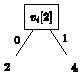
\includegraphics[scale=2.5]{chapters/mining/mining-ethereum-figures/dectree.pdf}
\end{minipage}
\caption{The classification problem is based on the gas used by $\tx_3$ (left) and the resulting decision tree (right).} 
\label{fig:mining-ethereum-dectree}
\end{figure}


\paragraph{Step (3): Extracting Gas Usage Rules} Now that we have estimated the neighborhood of every transaction, our next goal is to extract a set of rules that define the gas usage of each transaction $\tx$ based on the subset of neighbors that precede $\tx$ in the block and their order of appearance.


\paragraph{Syntax} Our rules are defined by the grammar below:
\begin{equation} \label{eq:ethereum-mining-grammar}
\begin{matrix*}[l]
\langle \text{predicate} \rangle & :=  &   \has \tx ~|~  \tx \before \tx ~|~ \neg \langle \text{predicate} \rangle \\
\langle \text{predicate-list} \rangle & :=  & \langle \text{predicate} \rangle ~|~ \langle \text{predicate} \rangle, \langle \text{predicate-list} \rangle    \\
\langle \text{clause} \rangle  & := &  \langle \text{predicate} \rangle ~|~  \atleast(k, \langle \text{predicate-list} \rangle) ~|~\\
& &  \langle \text{clause} \rangle \land \langle \text{clause} \rangle \\
\langle \text{rule} \rangle & := & \langle \text{clause} \rangle  \Rightarrow \expgas(\tx) = g\\
& &g, k \in \mathbb N, \tx \in \pool
\end{matrix*}
\end{equation}



\paragraph{Semantics} Given a sequence of distinct transactions $\pi = \langle \pi[1], \ldots, \pi[m]\rangle, $ we have:
\begin{equation} \label{eq:ethereum-mining-semantics}
\begin{matrix*}[l]
	\pi \models \has\tx_i & \Leftrightarrow & \exists i' ~~ (\pi[i'] = \tx_i) \\
	 \pi \models \tx_i \before \tx_j & \Leftrightarrow & \pi \not\models \has\tx_j \lor \exists i', j' ~~ (i'<j' \land  \\
	 &&\pi[i'] = \tx_i \land \pi[j'] = \tx_j)\\

	 \pi \models \neg p & \Leftrightarrow & \pi \not\models p\\
	 \pi \models c_1 \land c_2 & \Leftrightarrow & \pi \models c_1 \land \pi \models c_2\\
	 \pi \models \atleast(k, p_1, \ldots, p_m) & \Leftrightarrow & \exists i_1, \ldots, i_k ~~ (1 \leq i_1 < \ldots < i_k \leq m \land \\
	 &&\forall j ~~ \pi \models p_{i_j})
\end{matrix*}
\end{equation}

Intuitively, $\pi$ satisfies the predicate $\has \tx_i$ if it includes $\tx_i.$ It satisfies the predicate $\tx_i \before \tx_j$ if it either excludes $\tx_j$ altogether or has $\tx_i$ preceding $\tx_j.$ A clause is simply a conjunction of predicates. We also allow clauses of the form $\atleast(k, p_1, \ldots, p_m)$ which require $\pi$ to satisfy at least $k$ of the predicates $p_1, \ldots, p_m.$ Although the latter could be left as syntactic sugar, including it as a separate clause is helpful in practice. This is because of a common scenario in smart contracts, especially those modeling NFT or token giveaways, in which the first $k$ transactions to call a function can receive the token. In such cases, all transactions calling this function are dependent in terms of gas, but the gas usage of each of them is only dependent on how many other transactions precede it.  Finally, a rule of the form $C \Rightarrow \expgas(\tx_i) \geq g$ signifies a prediction: if $C$ is satisfied, we expect the gas usage of the transaction $\tx_i$ to be at least $g.$



\paragraph{Step (3.i): Generating a Decision Tree}  In this step, we generate a set of rules for each transaction $\tx_i \in \pool.$ We process each such transaction separately. When generating the rules for $\tx_i,$ we narrow our focus down to its neighborhood $\nbhd(\tx_i)$ since we believe these are the only transactions that can affect the gas usage of $\tx_i.$ Let $\pi_j$ be one of the sample permutations. We define $\pi_j^*$ as the subsequence of $\pi_j$ induced by $\nbhd(\tx_i) \cup \{\tx_i\},$ i.e.~the subsequence obtained by removing every element that is not in the neighborhood or not $\tx_i$ itself. If $\pi \not\models \has \tx_i,$ we ignore this sample as it does not include $\tx_i$ and cannot give us any information about its gas usage. We use $\Pi^*$ to denote the set of neighborhood-induced samples.
 
 As in Step 2, our goal is to form a decision tree that predicts the gas usage of $\tx_i$ based on features that encode the set of neighbors that precede it in the block and their order. Thus, for every neighboring $\tx_j \in \nbhd(\tx_i)$ we define a corresponding feature
 $$
 w[j] = \left\{ 
 	\begin{matrix}
 		j' - i' &  \text{if }\pi^* \models \tx_j \before \tx_i \land \pi^*[i']=\tx_i  \land \pi^*[j'] = \tx_j \\
 		0 & \text{otherwise}
 	\end{matrix}
 	\right..
 $$   
 Informally, if $\pi^*$ puts $\tx_j$ before $\tx_i,$ then $-w[j]$ is the distance between the two transactions in $\pi^*.$ Otherwise, $w[j]=0.$ In other words, we care about the distance only if $\tx_j$ precedes $\tx_i.$ This is because if $\tx_j$ does not appear before $\tx_i,$ it cannot affect $\tx_i$'s gas usage.  In addition to the $w[j]$'s, we also add an extra feature $r$ which models the number of neighbors that precede $\tx_i,$ or equivalently, the index in $\pi^*$ at which $\tx_i$ appears. We generate a decision tree using the same method as in Step 2, where the samples are the subsequences $\pi^*,$ the features are $r$ and the $w[j]$'s, and the labels are different possible gas usage values of $\tx_i.$ Note that our features are no longer binary. 

% Questions: Why do we need r? Why did we come up with this vectors?

\paragraph{Example} For step 2 of the algorithm in our previous example, suppose we know that $\nbhd(\tx_1) = \{\tx_4, \tx_5\}$. Then for $\pi_1 = \langle \tx_4,\tx_5, \tx_1, \tx_2, \tx_3, \tx_6\rangle$ the induced sample is $\pi_1^* = \langle \tx_4, \tx_5, \underline{\tx_1} \rangle.$ The encoding $w[\tx_4] = 0 - 2$ as the position of $\tx_4$ is $0$ and the position of $\tx_1$ is $2.$ Similarly, $w[\tx_5] = 1 - 2 = -1$ and $w[\tx_1] = 2 - 2 = 0.$ The feature $w[r] = 2$ as the number of neighbors that precede $\tx_1$ is $2.$ The encoding of the rest of the samples is shown in Figure~\ref{fig:mining-ethereum-dectree-2}.


\newcommand{\fmmmm}{\mspace{1mu}} %fake minus
\newcommand{\fmmm}{\mspace{2mu}} %fake minus


\newcommand{\fm}{\mspace{12mu}} %fake minus
\newcommand{\fmm}{\mspace{11mu}} %fake minus

\newcommand{\fmz}{\mspace{9mu}} %fake minus
\newcommand{\fma}{\mspace{10mu}} %fake minus
\newcommand{\fmb}{\mspace{11mu}} %fake minus
\newcommand{\fmc}{\mspace{12mu}} %fake minus
\newcommand{\fmd}{\mspace{13mu}} %fake minus
\newcommand{\fme}{\mspace{14mu}} %fake minus

\begin{figure}
\centering
{
\small
\begin{tabular}{|c|c|c|c|}
\hline
\shortstack{Sample\\($\pi_i$)} & \shortstack{nbhd($\tx_1$)-induced \\ Sample ($\pi^*_i$)} & \shortstack{Encoding ($w$)\\$|\pi_1, \pi_4, \pi_5, r\mspace{1mu}|$} & \shortstack{Label\\$(\tx_1$'s gas)}\\ \hline\hline
$\pi_1$    & $\langle\tx_4, \tx_5, \underline{\tx_1} \rangle$ &  $[0,   -2,    -1,2]$       & $ 6$\\
$\pi_2$    & $\langle\tx_4, \underline{\tx_1}, \tx_5 \rangle$ &  $[0,   -1, \fmb 0,1]$      & $ 8$\\
$\pi_3$    & $\langle\underline{\tx_1}, \tx_5, \tx_4 \rangle$ &  $[0,\fmb 0,\fmb 0,0]$      & $10$\\
$\pi_4$    & $\langle\tx_4, \underline{\tx_1}, \tx_5 \rangle$ &  $[0,   -1, \fmb 0,1]$      & $ 8$\\
$\pi_5$    & $\langle\tx_4, \tx_5, \underline{\tx_1} \rangle$ &  $[0,   -2,    -1,2]$       & $ 6$\\
$\pi_6$    & $\langle\tx_4, \underline{\tx_1}, \tx_5 \rangle$ &  $[0,  \fmmm -1, \fma 0,1]$ & $ 8$\\
$\pi_7$    & $\langle\tx_5, \underline{\tx_1}, \tx_4 \rangle$ &  $[0,\fm 0,    -1,1]$       & $ 2$\\
$\pi_8$    & $\langle\underline{\tx_1}, \tx_4, \tx_5 \rangle$ &  $[0,\fmb 0,\fmc 0,0]$      & $10$\\
$\pi_9$    & $\langle\tx_5, \underline{\tx_1}, \tx_4 \rangle$ &  $[0,\fm 0,   -1,  1]$        & $ 2$\\
$\pi_{10}$ & $\langle\underline{\tx_1}, \tx_5, \tx_4 \rangle$ &  $[0,\fmb 0,\fmc 0,0]$      & $10$\\ 
\hline
\end{tabular}
}
\caption{The classification problem  based on the gas used by $\tx_1$}
\label{fig:mining-ethereum-dectree-2}
\end{figure}




\paragraph{Step (3.ii): Extracting Rules from the Decision Tree} In the decision tree generated for $\tx_i$ in Step (3.i), every leaf is labeled by one possible gas usage value of $\tx_i.$ Let $\ell$ be a leaf labeled by $g_\ell$. Consider a feature $w[j].$ We know that $-n \leq w[j] \leq 0.$ In the path from the root of the decision tree to the leaf $\ell,$ some decisions bound $w[j]$ from above or below. Let $m_j$ be the largest lower-bound and $M_j$ the smallest upper-bound imposed on $w[j]$ in the root-to-leaf path ending at $\ell.$ Thus, in all samples modeled by this leaf, we have $w[j] \in [m_j, M_j].$ Similarly, we can define the tightest possible segment $[m_r, M_r]$ for values of $r$ in these samples. For each leaf $\ell,$ we generate a gas usage rule containing a clause $\varphi_\ell$ as follows:
\begin{itemize}
	\item We add the conjunct $\has \tx_i$ to $\varphi_\ell.$
	\item If for two transactions $\tx_j, \tx_{j'} \in \nbhd(\tx_i),$ we have $M_j \leq m_{j'},$ then $\tx_j$ is always preceding $\tx_{j'}$ in the samples corresponding to $\ell.$ Thus, we add the conjunct $\tx_j \before \tx_{j'}$ to $\varphi_\ell.$ 
	\item If for a transaction $\tx_j \in \nbhd(\tx_i),$ we have $m_j \geq 0,$ then $\tx_j$ is never appearing before $\tx_i$ in the samples corresponding to $\ell.$ Thus, we add the conjunct $\tx_i \before \tx_j$ to $\varphi_\ell.$
	\item If $m_r > 0,$ then in every sample corresponding to $\ell,$ at least $m_r$ neighboring transactions preceded $\tx_i.$ Let the neighborhood of $\tx_i$ be $\nbhd(\tx_i) = \{\tx_{j, 1}, \ldots, \tx_{j, q}\}.$ To capture this, we add the conjunct $\atleast(m_r, \tx_{j, 1} \before \tx_i, \ldots, \tx_{j, q} \before \tx_i)$ to $\varphi_\ell.$ 
	\item Similarly, if $\nbhd(\tx_i) = \{\tx_{j, 1}, \ldots, \tx_{j, q}\}$ and $M_r < q,$ then at most $M_r$ neighbors precede $\tx_i$ in each of the samples corresponding to $\ell.$ Therefore, $\tx_i$ precedes at least $q-M_r$ neighbors in each such sample. Hence, we add the conjunct $\atleast(q-M_r, \tx_i \before \tx_{j, 1}, \ldots, \tx_i \before \tx_{j, q})$ to the clause $\varphi_\ell.$
\end{itemize}
By definition-chasing, it is easy to prove that for every sample $\pi^*$ corresponding to the leaf $\ell$ of the decision tree, we have $\pi^* \models \varphi_\ell.$ Hence, one might assume that the expected gas usage of $\tx_i$ in a sample satisfying $\varphi_\ell$ is the same as $\ell$'s label $g_\ell.$ However, $\varphi_\ell$ might be satisfied by other samples, i.e.~samples corresponding to other leaves, too. This is rare in practice, but to handle it, our algorithm takes the average gas usage of $\tx_i$ over \emph{all} samples $\pi^*$ that model $\varphi_\ell.$ Formally, let $J = \{ j ~|~ 1 \leq j \leq k  \land \pi^*_j \models \varphi_\ell \}.$ Our algorithm computes
$$
\overline{g}_\ell = \frac{\sum_{j \in J} \gas(\pi_j, \tx_i) }{|J|}.
$$
In almost all real-world cases, we have $\overline{g}_\ell = g_\ell.$ Finally, our algorithm generates the following gas usage rule:
\begin{equation} \label{eq:mining-ethereum-gur}
\varphi_\ell \Rightarrow \expgas(\tx_i) = \overline{g}_\ell.
\end{equation}
We remark that for each transaction $\tx_i$ and every leaf $\ell$ of the decision tree corresponding to $\tx_i,$ our algorithm generates one instance of the gas usage rule in Equation~\eqref{eq:mining-ethereum-gur}.

\paragraph{Example} Let Figure \ref{fig:mining-ethereum-dectree-final} be the decision tree generated for $\tx_1$ in our previous example. The tree has $6$ leaves $l_1$ -- $l_6$ labelled $10, 2, 10, 8, 6, 6$ respectively. Consider the leaf $l_5$, taking the negations into the account, the predicates along the path evaluate to: $w[\pi_4] < 0.0$, $w[\pi_5] \geq -1.5$, $w[\pi_4] < -1.5$, which after rounding to integers, gives us the intervals $w[\pi_4] \in (-\infty, -2] = (m_4, M_4]$, $w[\pi_5] \in [-1, \infty) = [m_5, M_5)$. Notice that $M_4 \leq 0$ which generates the clause $\tx_4 \before tx_1$, and $M_4 \leq m_5$ which generates the clause $\tx_4 \before \tx_5$. Therefore, the rule's body is $\has \tx_1 \land (\tx_4 \before \tx_1) \land (\tx_4 \before \tx_5)$. Observe that  $\{\pi_1, \pi_2, \pi_4, \pi_5, \pi_6\} \models \has \tx_1 \land (\tx_4 \before \tx_1) \land (\tx_4 \before \tx_5)$, with average gas usage of $\tx_1$ equal to $(6 + 8 + 8 + 6 + 8)/5 = 7.2$. The remaining rules are given in Figure \ref{fig:mining-ethereum-rules}. 

Notice that no permutation can satisfy the rule $l_4$ and we assign the undefined $\bot$ average usage to it. We exclude such rules from consideration in the rest of the algorithm.


\begin{figure}
\centering
\begin{forest}
[
$w {[\pi_4]}$ $ \geq 0.0$
	[
	$w{[\pi_5]}$ $ \geq 0.0$
		[$l_1$: $10$]
		[$l_2$: $2$]
	]
	[
	$w{[\pi_5]}$ $ \geq -1.5$
		[
		$w{[\pi_4]}$ $ \geq -1.5$
			[$w{[\pi_5]}$ $ \geq 0.0$
			[$l_3$: $8$]
			[$l_4$: $6$]
			]
			[$l_5$: $6$]
		]
		[$l_6$: $6$]
	]
]
\end{forest}
\caption{The resulting decision tree for $\tx_1$.}
\label{fig:mining-ethereum-dectree-final}
\end{figure}

\begin{figure}
    \newcommand{\shiftleft}{\mspace{-50mu}} 

    \begin{equation*} 
        \begin{matrix}
            & m_4,M_4 & m_5,M_5 && \textup{rule} & & \shiftleft \expgas(\tx_1)\\
l_1: & [0, \infty)& [0, \infty) && \has \tx_1 \land (\tx_1 \before \{\tx_4, \tx_5\})& \Rightarrow &  10 \\
l_2: & [0, \infty)& (-\infty, -1] && \has \tx_1 \land (\tx_1 \before \tx_4) \land (\tx_5 \before \tx_1) & \Rightarrow &  2 \\
l_3: & [-1, -1]& [0, \infty) && \has \tx_1 \land (\tx_4 \before \tx_1) \land (\tx_1 \before \tx_5) & \Rightarrow &  8 \\
l_4: & [-1, -1]& [-1, -1] && \has \tx_1\land (\{\tx_4,\tx_5\} \before \tx_1)\land   & \Rightarrow &  \bot \\
&&&&(\tx_4 \before \tx_5) \land (\tx_5 \before \tx_4) && \\
l_5: & (-\infty, -2]& [-1, \infty) && \has \tx_1 \land (\tx_4 \before \tx_1) \land (\tx_4 \before \tx_5) & \Rightarrow &  7.2 \\
l_6: & (-\infty, -1]& (-\infty, -2] && \has \tx_1 \land (\{\tx_4, \tx_5\} \before \tx_1)  & \Rightarrow &  6 \\
\end{matrix}
\end{equation*}
\caption{The gas usage rules generated for $\tx_1$.}
\label{fig:mining-ethereum-rules}
\end{figure}


\begin{theorem}
	\label{thm:mining-ethereum-sufficient-samples}
	
	Assume there are no nonce dependencies and the neighborhood of every transaction is known. Consider the following stochastic process: We start with an empty sample set. In each step, we uniformly sample a new permutation of the transactions in $\pool$ and add it to $\Pi$. The process stops at the moment $T$ when the sample set $\Pi$ becomes sufficient. Then,  for any $\varepsilon \in (0, 1)$, the following holds:
	\[
        \PP{T < \Delta! \cdot \log \frac{|\pool| \cdot (\Delta + 1)!}{\varepsilon}} \geq 1 - \varepsilon.
	\]
\end{theorem}
\begin{proof}[Proof of \Cref{thm:mining-ethereum-sufficient-samples}]
For a transaction $\tx$, the probability that an induced permutation $\pi^*$ does not appear after one step is 
$
1 - \frac{1}{(|\nbhd(\tx)| + 1)!} \leq 1 - \frac{1}{(\Delta + 1)!}.
$
By the independence of trials, the probability that the induced permutation remains unseen after $r$ steps is 
$
\left(1 - \frac{1}{(\Delta + 1)!}\right)^r \leq \exp\left(-\frac{r}{(\Delta + 1)!}\right).
$
As for each $\tx$ there are at most $(\Delta + 1)!$ induced blocks, by the union bound, the probability that there exists a transaction $\tx$ such that the induced permutation $\pi^*$ does not appear after $r$ steps is at most 
$
	\PP{T \geq r} \leq |\pool| \cdot (\Delta + 1)! \cdot \exp\left(-\frac{r}{(\Delta + 1)!}\right).
$
After plugging in
$
r = (\Delta + 1)! \cdot \log \left(\frac{|\pool| \cdot (\Delta + 1)!}{\varepsilon}\right),
$
and rearranging the terms, we obtain the desired result.

\end{proof}	

\section{Runtime and Revenue Results on Ethereum}\label{sec:mining-ethereum-experiments}

\paragraph{Implementation}
We implemented our approach in Python 3 and Rust. Our tool is open-access and available online. We used Anvil~\cite{foundry2023anvil} and Erigon~\cite{erigontech2023erigon} to execute Ethereum transactions in our samples and to obtain their gas usage. Moreover, we used Linfa~\cite{linfa2025linfa} to generate decision trees and relied on SCIP~\cite{bolusani2024scip} to solve Integer Linear Programming (ILP) instances.


\paragraph{Machine} All experimental results were obtained on an Intel Xeon Gold 5115 Machine (2.40GHz, 16 cores) with 64 GB of RAM, running Ubuntu 22.04.

\paragraph{Benchmarks}
As our benchmark suite, we collected a dataset of real-world mempools, i.e.~ unmined transactions, that were available on the Ethereum network before each block. Our data spans 50,000 blocks, numbered 21800000 to 21849999, corresponding to approximately one week of activity on Ethereum in the period from February 8, 2025, 06:27:11 (UTC) to February 15, 2025, 06:18:35 (UTC). This data was gathered from Blocknative~\cite{blocknative2025mempool}. 

\paragraph{Samples and Runtime} For each of the 50,000 blocks, we generated 300 sample permutations and limited our solver's execution time to 12 seconds, i.e.~Ethereum's block time. We note that the results were obtained on a relatively modest machine. The testing and decision-tree generation steps of our algorithm are parallelized, thus increasing the computational power would allow one to cover more samples for each block. We expect real-world miners to have much higher computational power than us.

\paragraph{Baselines} For each block, we compare the total tip revenue obtained by our approach with the real-world block that was mined and added to the Ethereum blockchain. In the experiments, we observed that some Ethereum miners routinely miss lucrative transactions when forming their blocks. This might be due to a suboptimal block formation strategy or network connectivity issues that prevented the miner from seeing the transactions, e.g.~due to the censorship of the Ethereum network in some countries. Thus, it is conceivable that the miner might not have the same mempool as us. We believe this does not affect the fairness of the comparison since the onus is on the miners to ensure they have reliable connectivity to the network. However, to demonstrate that our improvements are not merely due to better connectivity, as a second baseline, we used Ethereum's reference implementation and applied it to the exact same mempools as our algorithm. The reference implementation sorts transactions greedily based on their effective gas tip value, prioritizing transactions with higher tips for miners and ordering same-sender transactions by nonce~\cite{foundry2023anvil, foundation2025go}.




\begin{table}[!htbp]
\centering
\caption{Improvements obtained by our approach compared to real-world miners and the Ethereum reference implementation.}
\label{table:mining-ethereum-comparisonBaseline}
\renewcommand{\arraystretch}{1.2}
\begin{tabular}{|>{\raggedright\arraybackslash}p{0.32\textwidth}|>{\raggedright\arraybackslash}p{0.32\textwidth}|>{\raggedright\arraybackslash}p{0.32\textwidth}|}
\hline
\textbf{Metric} & Improvement compared to Real-World Miners & Improvement compared to Reference Implementation \\
\hline\hline
Number of improved blocks & 45{,}609 (91.22\%) & 38{,}505 (77.01\%) \\ \hline
Total increase in tip revenue over 50{,}000 blocks & 1{,}204{,}475 USD & 863{,}385 USD \\ \hline
Annualized increase in tip revenue & 63{,}357{,}892 USD & 45{,}416{,}764 USD \\ \hline
Average earning increase per block & 24.1 USD & 17.3 USD \\ \hline
Average improvement percentage per block & 73.45\% & 18.56\% \\ 
\hline
\end{tabular}
\renewcommand{\arraystretch}{1}
\end{table}

% Question why going from 18 percent to 73 percent does not make a huge different in USD?

\paragraph{Revenue Gains}
 The revenue gains obtained by our algorithm are summarized in Table~\ref{table:mining-ethereum-comparisonBaseline} and Figure~\ref{fig:mining-ethereum-revenueComparisionWReal}. Our approach outperformed real-world miners in 45,609 of the 50,000 blocks (91\% of the cases), increasing the total revenue over all blocks by \textbf{1,204,475 USD}\footnote{We used the ETH/USD conversion rates provided by~\cite{coinmarketcap2025cryptocurrency}.}. On average, this represents an increase of nearly 24.1 USD per block, which translates to an annualized improvement of around \textbf{63 million USD} . Our approach obtained significant gains compared to the Ethereum reference implementation, as well. It outperformed the reference implementation in 38,505 blocks (77\% of the cases), yielding an additional revenue of \textbf{863,385 USD} over our 50,000 benchmark blocks. This translates to approximately \textbf{45 million USD} annually. On average, our algorithm earned almost 17.3 USD more per block. The data in Table~\ref{table:mining-ethereum-comparisonBaseline} should be taken with the usual grains of salt: (i)~Ether's value and its exchange rate to USD are highly volatile and unpredictable, and (ii)~the reported numbers are the sums of improvements over individual blocks. Figures~\ref{fig:mining-ethereum-revenueIncreaseReal} and~\ref{fig:mining-ethereum-revenueIncreaseGreedy} and provide histograms of the gained revenues in USD.  Figures~\ref{fig:mining-ethereum-percentageImprovementOverReal} and~\ref{fig:mining-ethereum-percentageImprovementOverGreedy} show similar histograms based on the percentage of improvement obtained in each block.



 \begin{figure}[ht]
	\centering
	\includegraphics[width=0.6\columnwidth]{chapters/mining/mining-ethereum-figures/revenueComparisionWReal.pdf}
	\caption{
		Comparison of the tip revenues obtained by our algorithm (x-axis) and the real-world blocks added to the Ethereum blockchain (y-axis). Each point corresponds to one block. Green points (91.22\%) are the blocks on which our algorithm obtained a higher revenue than real-world miners. For clarity, we excluded 265 data points.} 
	\label{fig:mining-ethereum-revenueComparisionWReal}
\end{figure}


\begin{figure}[ht]
	\centering
	\includegraphics[width=0.8\columnwidth]{chapters/mining/mining-ethereum-figures/revenueImprovementReal.pdf}
	\caption{Histogram of the transaction fee improvements obtained over each block compared to real-world miners (in USD). The y-axis is in logarithmic scale. For clarity, 411 data points outside the range are omitted.}
	\label{fig:mining-ethereum-revenueIncreaseReal}
\end{figure}



\begin{figure}[ht]
    \centering
    \includegraphics[width=0.8\columnwidth]{chapters/mining/mining-ethereum-figures/revenueImprovementGreedy.pdf}
    \caption{Histogram of the transaction fee improvements obtained over each block compared to the Ethereum reference implementation (in USD). The y-axis is in logarithmic scale. For readability, 868 blocks with improvements over 150 USD are omitted from the plot.}
    \label{fig:mining-ethereum-revenueIncreaseGreedy}
\end{figure}


\begin{figure}[ht]
	\centering
	\includegraphics[width=0.8\columnwidth]{chapters/mining/mining-ethereum-figures/percentageImprovementOverReal.pdf}
	\caption{Histogram of the transaction fee improvements obtained over each block compared to real-world miners (in percentages). 608 points outside the range omitted for clarity.}
	\label{fig:mining-ethereum-percentageImprovementOverReal}
\end{figure}



\begin{figure}[ht]
    \centering
    \includegraphics[width=0.8\columnwidth]{chapters/mining/mining-ethereum-figures/percentageImprovementOverGreedy.pdf}
    \caption{Histogram of the transaction fee improvements obtained over each block compared to the Ethereum reference implementation (in percentages). The y-axis is in logarithmic scale. 2021 points outside the range omitted for clarity.}
    \label{fig:mining-ethereum-percentageImprovementOverGreedy}
\end{figure}



\paragraph{Sample Size Sensitivity} To investigate the effect of sample size on our approach, we reran our experiments with sample sizes of $50$, $100$, $200$, and $300$. The improvement in revenue slows as sample size increases. We observed that the marginal gain from $200$ to $300$ samples is less pronounced. See Table~\ref{table:mining-ethereum-parametersensitivity} for details. Moreover, the average neighborhood size is $1.21$, which, according to Theorem~\ref{thm:mining-ethereum-sufficient-samples}, indicates that relatively small sample sizes suffice.

\begin{table}
\centering

\caption{Pairwise differences in annualized revenue across sample sizes of 50, 100, 200, and 300 in thousands of USD.}

\label{table:mining-ethereum-parametersensitivity}
\begin{tabular}{|c|c|c|c|c|}
\hline
\makecell{\textbf{Sample Size}} & \makecell{\textbf{50}} & \makecell{\textbf{100}} & \makecell{\textbf{200}} & \makecell{\textbf{300}} \\
\hline\hline
50 & 0 & -1457.53 & -2910.24 & -3253.29 \\
\hline
100 & 1457.53 & 0 & -1452.71 & -1795.76 \\
\hline
200 & 2910.24 & 1452.71 & 0 & -343.047 \\
\hline
300 & 3253.29 & 1795.76 & 343.047 & 0 \\
\hline
\end{tabular}

\end{table}



\paragraph{Runtime Performance} In practice, executing one block sample took 2.42 seconds on average. The end-to-end processing took an average of 5.7 seconds (without parallelization). Moreover, the pure ILP solving time (Step 5) was only 0.4 seconds.
Refer to Figures~\ref{fig:mining-ethereum-HistogramIlpOnEndToEndOverlay} for details.
We emphasize that steps 2-4 can be parallelized, allowing for runtime reduction with additional computational power. The ILP performance depends primarily on instance sparsity rather than mempool size. We observed that increasing the number of transactions in the mempool leads to ILP instances that are easier and faster to solve. See Figure~\ref{fig:mining-ethereum-ScatterIlpTimeTxCountSampleSize300} for details.



\begin{figure}[ht]
    \centering
    \includegraphics[width=0.8\columnwidth]{chapters/mining/mining-ethereum-figures/HistogramIlpOnEndToEndOverlay.pdf}
	\caption{Histogram of the end-to-end (green) and ILP solver (blue) processing times per block. The y-axis is in logarithmic scale.}
	\label{fig:mining-ethereum-HistogramIlpOnEndToEndOverlay}
\end{figure}


\begin{figure}[ht]
	\centering
	\includegraphics[width=0.8\columnwidth]{chapters/mining/mining-ethereum-figures/ScatterIlpTimeTxCountSampleSize300.pdf}
	\caption{Scatter of ILP solver time (seconds) versus number of transactions per mempool, with sample size fixed at 300.}
	\label{fig:mining-ethereum-ScatterIlpTimeTxCountSampleSize300}
\end{figure}


% \begin{figure}[h]
% 	\centering
% 	\begin{subfigure}[b]{0.48\textwidth}
% 		\centering
% 		\includegraphics[width=\textwidth]{chapters/mining/mining-ethereum-figures/ScatterIlpTimeTxCountSampleSize50.pdf}
% 		\subcaption{Sample size 50}
% 		\label{fig:ScatterIlpTimeTxCountSampleSize50}
% 	\end{subfigure}
% 	\hfill
% 	\begin{subfigure}[b]{0.48\textwidth}
% 		\centering
% 		\includegraphics[width=\textwidth]{chapters/mining/mining-ethereum-figures/ScatterIlpTimeTxCountSampleSize100.pdf}
% 		\subcaption{Sample size 100}
% 		\label{fig:ScatterIlpTimeTxCountSampleSize100}
% 	\end{subfigure}
	
% 	\begin{subfigure}[b]{0.48\textwidth}
% 		\centering
% 		\includegraphics[width=\textwidth]{chapters/mining/mining-ethereum-figures/ScatterIlpTimeTxCountSampleSize200.pdf}
% 		\subcaption{Sample size 200}
% 		\label{fig:ScatterIlpTimeTxCountSampleSize200}
% 	\end{subfigure}
% 	\hfill
% 	\begin{subfigure}[b]{0.48\textwidth}
% 		\centering
% 		\includegraphics[width=\textwidth]{chapters/mining/mining-ethereum-figures/ScatterIlpTimeTxCountSampleSize300.pdf}
% 		\subcaption{Sample size 300}
% 		\label{fig:ScatterIlpTimeTxCountSampleSize300A}
% 	\end{subfigure}
	
% 	\caption{\added{Scatter of ILP solver time (seconds) versus number of transactions per mempool for different sample sizes.}}
% 	\label{fig:ScatterIlpTimeTxCount}
% \end{figure}

% \clearpage
% \begin{figure}[h]
% 	\centering
% 	\begin{subfigure}[b]{0.48\textwidth}
% 		\centering
% 		\includegraphics[width=\textwidth]{chapters/mining/mining-ethereum-figures/ScatterIlpTimeByAvgNeighborhoodSampleSize50.pdf}
% 		\subcaption{Sample size 50}
% 		\label{fig:ScatterIlpTimeByAvgNeighborhoodSampleSize50A}
% 	\end{subfigure}
% 	\hfill
% 	\begin{subfigure}[b]{0.48\textwidth}
% 		\centering
% 		\includegraphics[width=\textwidth]{chapters/mining/mining-ethereum-figures/ScatterIlpTimeByAvgNeighborhoodSampleSize100.pdf}
% 		\subcaption{Sample size 100}
% 		\label{fig:ScatterIlpTimeByAvgNeighborhoodSampleSize100A}
% 	\end{subfigure}
	
% 	\begin{subfigure}[b]{0.48\textwidth}
% 		\centering
% 		\includegraphics[width=\textwidth]{chapters/mining/mining-ethereum-figures/ScatterIlpTimeByAvgNeighborhoodSampleSize200.pdf}
% 		\subcaption{Sample size 200}
% 		\label{fig:ScatterIlpTimeByAvgNeighborhoodSampleSize200A}
% 	\end{subfigure}
% 	\hfill
% 	\begin{subfigure}[b]{0.48\textwidth}
% 		\centering
% 		\includegraphics[width=\textwidth]{chapters/mining/mining-ethereum-figures/ScatterIlpTimeByAvgNeighborhoodSampleSize300.pdf}
% 		\subcaption{Sample size 300}
% 		\label{fig:ScatterIlpTimeByAvgNeighborhoodSampleSize300A}
% 	\end{subfigure}
	
% 	\caption{\added{Scatter of ILP solver time (seconds) versus average neighborhood size per block for different sample sizes.}}
% 	\label{fig:ScatterIlpTimeByAvgNeighborhood}
% \end{figure}

% \begin{figure}[h]
% 	\centering
% 	\begin{subfigure}[b]{0.48\textwidth}
% 		\centering
% 		\includegraphics[width=\textwidth]{chapters/mining/mining-ethereum-figures/HistogramNeighborhoodSizeSampleSize50.pdf}
% 		\subcaption{Sample size 50}
% 		\label{fig:HistogramNeighborhoodSizeSampleSize50A}
% 	\end{subfigure}
% 	\hfill
% 	\begin{subfigure}[b]{0.48\textwidth}
% 		\centering
% 		\includegraphics[width=\textwidth]{chapters/mining/mining-ethereum-figures/HistogramNeighborhoodSizeSampleSize100.pdf}
% 		\subcaption{Sample size 100}
% 		\label{fig:HistogramNeighborhoodSizeSampleSize100A}
% 	\end{subfigure}
	
% 	\begin{subfigure}[b]{0.48\textwidth}
% 		\centering
% 		\includegraphics[width=\textwidth]{chapters/mining/mining-ethereum-figures/HistogramNeighborhoodSizeSampleSize200.pdf}
% 		\subcaption{Sample size 200}
% 		\label{fig:HistogramNeighborhoodSizeSampleSize200A}
% 	\end{subfigure}
% 	\hfill
% 	\begin{subfigure}[b]{0.48\textwidth}
% 		\centering
% 		\includegraphics[width=\textwidth]{chapters/mining/mining-ethereum-figures/HistogramNeighborhoodSizeSampleSize300.pdf}
% 		\subcaption{Sample size 300}
% 		\label{fig:HistogramNeighborhoodSizeSampleSize300A}
% 	\end{subfigure}
	
% 	\caption{\added{Histogram of neighborhood size per block for different sample sizes.}}
% 	\label{fig:HistogramNeighborhoodSize}
% \end{figure}
\newpage

\chapter{Optimal Routing for Decentralized Exchanges}
\label{chp:hermes}
This chapter originally appeard in the following publication:

\begin{itemize}

    \item S. Farokhnia, S. Novozhilov, S. Safaei, J. Shen. \textit{Hermes: Scalable and Robust Structure-Aware Optimal Routing for Decentralized Exchanges}. IEEE International Conference on Blockchain, Blockchain 2025.

\end{itemize}


\newpage

\section{Introduction}

\para{Background} Decentralized exchanges (DEXs) have transformed the financial landscape by enabling transparent, permissionless token trading on blockchains. These platforms rely on smart contracts called liquidity pools. Each pool allows for the trading of two tokens, with the exchange price dynamically calculated by an automated algorithm based on the available liquidity. Uniswap, the leading DEX on Ethereum, features over 400,000 pools and tokens, supporting an average daily trading volume of \$1.3~\text{billion} USD since 2024. However, fragmentation across DEXs and the rapid growth in the number of tokens significantly complicate the search for optimal exchange rates, particularly when no direct trading pair exists. As a result, it often requires a sequence of trades across multiple pools, a challenge known as \emph{routing}.~Routing is typically modeled as a shortest path problem on a given graph of tokens. Existing algorithms have significant drawbacks: scalable approaches often lack guarantees for route validity, while robust methods struggle with the scale and dynamic nature of modern decentralized exchanges.

\para{Our Contributions} In this chapter, we address the problem of optimal routing on DEXs. We demonstrate that by leveraging the structural properties of this graph, in particular its \emph{treewidth}, it is possible to reconcile scalability with robustness. On the theoretical side, we adapt a parameterized algorithm utilizing treewidth to handle the dynamic setting of DEXs, where pools frequently change. We show that our approach achieves improved time complexity over existing methods and additionally provides a formal guarantee on the quality of the computed routes. We present empirical analysis on real Uniswap data to demonstrate the suitability of a parameterized online algorithm. Furthermore, we have implemented this algorithm in a free and open-source tool called Hermes and compared it with existing methods. On small instances where both tools produced results, Hermes reduced the average runtime by four orders of magnitude, from \todo{2.81} seconds to \todo{0.0002} seconds. Notably, Hermes is the only tool capable of computing routes in the presence of 100,000 tokens. It achieves an average runtime of \todo{0.19} seconds, while other approaches fail to complete within the allotted time.


\section{Exchange Rates as a Routing Problem}\label{sec:hermes-problem} 

\para{Decentralized Finance (DeFi)} Smart contracts have enabled the development of a new ecosystem that offers advanced, composable financial functions beyond basic token transfers on the blockchain, now collectively referred to as \emph{decentralized finance} (DeFi)~\cite{DBLP:conf/uss/McLaughlinKV23}.
DeFi has grown rapidly due to its transparent, trustless, and programmable financial services. Currently, the total value locked (TVL)\footnote{Total value locked refers to the aggregate value of all assets deposited in smart contracts.} in DeFi on Ethereum alone exceeds 65.9 billion USD~\cite{defillama, DBLP:journals/csur/XuPCF23}.\footnote{All prices in this paper are reported as of 15-06-2025.}

\para{Decentralized Exchanges (DEX)} Decentralized exchanges (DEXs) are a cornerstone of the DeFi ecosystem, enabling the permissionless trading of digital assets. Among the different DEX types, \emph{Automated Market Makers} (AMMs) have emerged as the most widely adopted by nearly every metric~\cite{zhang2024improved}. Central to AMMs is the concept of a \emph{liquidity pool}: a smart contract that holds reserves of two (or more) tokens, enabling users to trade between them without intermediaries. The exchange rate between two tokens within a liquidity pool is autonomously determined by a function of the current reserves. Uniswap is the leading DEX by TVL on Ethereum. Since 2024, Uniswap has hosted an average daily trading volume of $1.3$ billion USD, with an all-time cumulative trading volume reaching $2.26$ trillion USD~\cite{defillama}.

\para{Routing in Decentralized Exchanges} A fundamental challenge within the DEX ecosystem is discovering optimal exchange rates, a problem necessitated by the decentralized and fragmented liquidity landscape. Often, a direct trading pair between two assets does not exist, requiring a trader to perform a sequence of trades across several liquidity pools, a process known as \emph{routing}. 
Routing can be modeled as a graph problem on $G = (V, E, w)$, where the vertices $V$ represent tokens, the edges $E$ correspond to liquidity pools connecting pairs of tokens, and the weights $w$ encode the spot exchange rates available for trading between those tokens. A route is a sequence of tokens whose cumulative edge weights determine the final exchange rate. The goal is to find the route between two tokens that yields the best price. 
A well-known special case of routing is \emph{arbitrage}, where a trader earns risk-free profit by exploiting price discrepancies for the same asset across different pools. This problem is commonly modeled as finding a negative-weight cycle in the aforementioned graph~\cite{zhang2024improved,DBLP:conf/uss/McLaughlinKV23}. Arbitrages have been studied exhaustively in the literature on DEX due to their risk-free profits\cite{DBLP:journals/csur/XuPCF23}. However, the reported arbitrages constitute only a small fraction of trades, accounting for approximately $11.71\%$ of daily volume on Uniswap~\cite{theUniswapSubgraph,defillama}.


\para{Algorithmic Challenges in Routing}
While financial arbitrage has been extensively studied in both traditional and decentralized markets~\cite{DBLP:journals/csur/XuPCF23,zhang2024improved}, research focused on optimal routing within decentralized exchanges remains comparatively limited. The existing body of work reveals two primary algorithmic challenges. First, our study shows that current routing algorithms scale poorly as the number of assets increases. This issue is particularly acute given the operational constraints of modern blockchains, such as Ethereum's 12-second block time, and the dynamic nature of the ecosystem, which features continuously changing prices. Second, the presence of arbitrage opportunities, which manifest as negative-weight cycles in the graph-based problem formulation, renders standard shortest-path algorithms such as Bellman-Ford incapable of finding optimal routes. This situation has led to a dichotomy in existing solutions: they are either general-purpose algorithms that guarantee optimality but are often too slow for practical on-chain execution, or they rely on heuristics that are faster but offer no formal guarantees on the quality of the route.

\para{Our Focus}
In this chapter, we bridge this gap by designing a \textit{parameterized algorithm} tailored to the structural properties of DEX transaction graphs~\cite{Cygan2015}. The design of such algorithms follows a paradigm that diverges from traditional runtime analysis. Instead of measuring performance solely against the input size, a parameterized algorithm's efficiency is also analyzed with respect to an additional structural property of the input, known as a \textit{parameter}. For graphs, a common and powerful parameter is \emph{treewidth}, which measures how closely a graph resembles a tree. Our central thesis is that real-world DEX transaction graphs exhibit low treewidth. By exploiting this structural property, we have developed an algorithm that is both \textit{theoretically sound}, due to its formal complexity analysis, and \textit{practically efficient}, a claim we substantiate through extensive experiments on real-world DEX data. This approach strikes a crucial balance, achieving provable optimality without sacrificing the performance required in the demanding DEX environment.
\section{Our Algorithm}\label{sec:hermes-algorithm} 

\subsection{Formulating DEX prices as a graph problem}
\para{Automated Market Makers}
An \textit{Automated Market Maker} (AMM) is a protocol for decentralized trading that replaces traditional order books with deterministic pricing algorithms~\cite{mclaughlin2023large}. In an AMM, prices are set by a mathematical function of the current token reserves in each liquidity pool. The most widely used class of AMMs is the \textit{Constant Function Market Maker} (CFMM), of which Uniswap is a prominent example.
In Uniswap V2, the CFMM uses the constant product formula, which maintains a constant product of the reserves of two tokens $u$ and $v$ in a liquidity pool: $R_u \cdot R_v = k$, where $k$ is a fixed constant. Here, $R_u$ and $R_v$ represent the current quantities (reserves) of tokens $u$ and $v$ held in the pool, respectively. This means that any trade will adjust the reserves of both tokens while keeping their product constant. The spot price from token $u$ to token $v$ is determined by the ratio of their reserves, specifically $\text{price}(u \to v) = \frac{R_v}{R_u}$. Uniswap V3 allows liquidity providers to concentrate capital within custom price ranges, increasing efficiency. Uniswap V4 introduces \textit{hooks} for customizable trading strategies and fee structures~\cite{adams2023uniswap}. All three versions are active on Ethereum.

For the scope of this paper, these versions share two pricing notions. The first is the \textit{spot price}, which depends on the current reserves and indicates the current market price. The second is the \textit{trade price}, which also accounts for the size of the trade. The applications of both concepts have been thoroughly studied in the literature~\cite{xu2023sok}. In this chapter, we focus on spot prices.


\para{Modeling the DEX Ecosystem as a Graph}
To analyze and optimize trade routing across a decentralized exchange ecosystem, we employ the abstraction of a weighted directed graph $G=(V, E, w)$. In this model, the set of vertices $V$ represents the universe of available tokens. A directed edge $(u, v) \in E$ exists if there is a liquidity pool capable of direct trading from token $u$ to token $v$. A path in this graph, which is a sequence of connected vertices, therefore corresponds to a multi-hop trade that converts a source token into a destination token through one or more intermediaries. 


\para{Shortest Path Formulation}
The objective in trade routing is to find a path that maximizes the product of exchange rates\footnote{We assume rates are adjusted for all transaction fees.}. Since standard shortest path algorithms are designed to minimize a sum of weights, we align our problem by defining the weight of an edge $(u, v)$ as the negative logarithm of the exchange rate: $w(u, v) = -\log(\text{price}(u \to v))$. In the case of multiple liquidity pools between two tokens, we choose one pool maximizing the exchange rate $\max \text{price}(u \to v)$, thus avoiding the necessity of considering the multi-edge graphs. This weight assignment converts the maximization of a product into the minimization of a sum, thereby reformulating the optimal routing task as a Single-Source Shortest Path (SSSP) problem. A critical consideration in this model is the presence of negative-weight cycles, which correspond to arbitrage opportunities: trading paths that start and end with the same token and yield a profit. Such cycles can lead to infinitely cheap paths, a complication that must be handled by the chosen algorithm.


\para{Graph Notation and Terminology}
To develop an algorithm that leverages the specific topology of the DEX graph, we must first establish a formal language for discussing its local properties. We define the \textit{neighborhood} of a vertex $v$, denoted $N(v)$, as the set of all vertices directly accessible from it $N(v) := \{u \mid (v, u) \in E\}$. Furthermore, for any subset of vertices $S \subseteq V$, the \textit{subgraph induced by S}, denoted $G[S]$, consists of the vertices in $S$ and all edges from the original graph that connect any two vertices in $S$: $G[S] := (S, E \cap (S \times S))$. 

\para{Tree Decompositions and Treewidth}
The efficiency of our algorithm hinges on a structural parameter known as \textit{treewidth}, which quantifies how ``tree-like'' a graph is. Formally, the treewidth of a graph $G=(V, E)$ is defined via a \textit{tree decomposition}; see Section~\ref{sec:prelim-parameters-treewidth} for the formal definition.

\para{Chordal Graphs and Chordal Completion}
Our algorithm operates not on the original graph $G$, but on a \textit{chordal supergraph} of it. A graph is chordal if every cycle of four or more vertices has an edge connecting two non-consecutive vertices (a chord). While most graphs are not chordal, any graph $G$ can be transformed into one by adding a set of ``fill-in'' edges to create a \textit{chordal completion}, $\widehat{G}$. A key result in graph theory states that the treewidth of a graph is intrinsically linked to its best chordal completion: $tw(G) = \min_{\widehat{G}} \omega(\widehat{G}) - 1$, where the minimum is taken over all chordal completions of $G$ and $\omega(\widehat{G})$ is the size of the largest clique in $\widehat{G}$. This relationship is fundamental to our approach.

\para{All-Pairs Shortest Paths via Directed Path Consistency}
The core of our algorithm is an efficient method for solving the All-Pairs Shortest Paths (APSP) problem on graphs with low treewidth. The method relies on enforcing \textit{Directed Path Consistency} (DPC) using a PEO. A weighted graph is DPC with respect to an ordering $\pi = (v_1, \dots, v_n)$ if for every triple of vertices $v_i, v_j, v_k$ with $i<j<k$, the path cost from $v_i$ to $v_k$ is no greater than the cost of the path through $v_j$; i.e., $w(v_i, v_k) \le w(v_i, v_j) + w(v_j, v_k)$.

Enforcing this property on an arbitrary graph with an arbitrary ordering takes $O(n^3)$ time. However, by using the PEO of a chordal completion $\widehat{G}$, the process can be dramatically accelerated. The algorithm iterates backward through the PEO (from $v_n$ to $v_1$), and at each step $v_k$, it only needs to check for path updates between pairs of neighbors of $v_k$ that appear earlier in the ordering. Because a PEO ensures these neighbors form a clique of size at most $\omega(\widehat{G})$, the complexity of enforcing DPC is reduced to $O(n \cdot \omega(\widehat{G})^2)$, which is equivalent to $O(n \cdot tw(G)^2)$. 

The advantage of the DPC property is that all shortest paths become bitonic: any shortest path from $u$ to $v$ consists of a segment where vertices decrease in the PEO order, followed by a segment where they increase. This structure allows SSSP queries to be answered efficiently in two passes over the PEO array, see Algorithm~\ref{alg:hermes-query-sssp} for details.

\subsection{The Algorithm Overview}

Our proposed algorithm transforms a general graph into a structure where shortest path queries can be answered with remarkable efficiency. This transformation is achieved through a multi-phase process, illustrated in Figure~\ref{fig:hermes-dpc-process-illustration}. The first three phases constitute an offline preprocessing stage, which is performed only once. The final phase is the online query stage, designed for rapid, repeated execution.

The main idea is to construct a chordal supergraph leveraging graph's tree decomposition. The chordal graph admits a Perfect Elimination Ordering (PEO). This ordering is then used to enforce Directed Path Consistency (DPC). The DPC property is used to answer the Single-Source Shortest Path (SSSP) queries efficiently. The algorithm is designed to handle graphs with negative-weight cycles, ensuring that the results are correct even in the presence of such cycles. The entire process is summarized in Algorithm~\ref{alg:hermes-framework}.

\begin{algorithm2e}[H]
\footnotesize
\setstretch{0.8}
\caption{Unified Algorithm for Treewidth-Based Batch SSSP Queries}
\label{alg:hermes-framework}
\KwIn{A weighted graph $G=(V, E, d)$, a set of source vertices $Q = \{s_1, \dots, s_q\}$}
\KwResult{A list of SSSP distance arrays $(D[s_1], \dots, D[s_q])$, where each $D[s_i]$ contains the distances from source $s_i$ to every vertex in $V$}

\tcp{Structural Preprocessing}
$T \gets \text{ComputeTreeDecomposition}(G)$\;\label{alg:hermes-line:decomp}
$(\widehat{G}, \pi) \gets \text{ComputeCompletionAndPEO}(T)$\;\label{alg:hermes-line:peo}

\tcp{Weights Preprocessing}
$d^* \gets \text{EnforceDPC}(\widehat{G}, \pi, d)$\;\label{alg:hermes-line:dpc}

\tcp{Process each SSSP query}
\For{$i \gets 1$ \KwTo $q$}{ \label{alg:hermes-line:loop}
    $D[s_i] \gets \textup{QuerySSSP}(\widehat{G}, d^*, s_i)$\;\label{alg:hermes-line:query}
}
\end{algorithm2e}


The correctness and efficiency of this framework are formalized in Theorem~\ref{thm:hermes-main}. 


\begin{theorem}[Complexity and Correctness]
\label{thm:hermes-main}
Let $G=(V,E,d)$ be a weighted graph with $n = |V|$ vertices and treewidth $tw(G)$. The algorithm described in Algorithm~\ref{alg:hermes-framework} has an overall preprocessing time of $O(n \cdot tw(G)^2)$ and answers each SSSP query in $O(n \cdot tw(G)^2)$ time.

For each source vertex $s_i \in Q$, the resulting distance array $D_i$ has the following properties for any target vertex $t \in V$:
\begin{itemize}
    \item If there are no negative-weight cycles on any path from $s_i$ to $t$, then $D[s_i][t]$ stores the correct shortest path distance from $s_i$ to $t$ in the original graph $G$.
    \item If there is a negative-weight cycle on a path from $s_i$ to $t$, the corresponding distance $D[s_i][t]$ will be less or equal to the shortest simple path (a path with no repeated vertices) distance from $s_i$ to $t$ in $G$.
\end{itemize}
\end{theorem}



\begin{figure}[]
    \centering
    
    \begin{subfigure}[t]{0.47\columnwidth}
        \centering
        \includegraphics[width=0.7\linewidth]{chapters/hermes/hermes-figures/input-G.pdf}
        \caption{The input graph $G$.}
        \label{fig:hermes-input-G}
    \end{subfigure}
    \hfill 
    \begin{subfigure}[t]{0.51\columnwidth}
        \centering
        \includegraphics[width=0.9\linewidth]{chapters/hermes/hermes-figures/tree-decomp.pdf}
        \caption{A tree decomposition of $G$.}
        \label{fig:hermes-tree-decomp}
    \end{subfigure}

    \vspace{1em}

    \begin{subfigure}[t]{0.8\columnwidth}
        \centering
        \includegraphics[width=0.9\linewidth]{chapters/hermes/hermes-figures/fillin-g.pdf}
        \caption{The chordal completion $\widehat{G}$ with fill-in edges (\textcolor{purple}{$\widehat{E}$}) added.}
        \label{fig:hermes-fillin-g}
    \end{subfigure}

    \caption{An illustration of the preprocessing pipeline for the treewidth-based routing algorithm.}
    \label{fig:hermes-dpc-process-illustration}
\end{figure}

\begin{example}[Input Graph]
    We illustrate the entire pipeline using the graph from Figure~\ref{fig:hermes-dpc-process-illustration}. The process begins with the graph $G$ in Figure~\ref{fig:hermes-dpc-process-illustration}(a). We chose the weights to be symmetric $d(u, v) = d(v, u)$ for simplicity of presentation, generally the algorithm does not require this. The graph has $7$ vertices $\{v_1, \dots, v_7\}$, the $v$s are omitted in the figure for clarity. The edges has the following weights: $d(v_1, v_2)=5$, $d(v_2, v_3)=1$, $d(v_2, v_6)=12$, $d(v_3, v_4)=2$, $d(v_4, v_5)=7$, $d(v_4, v_7)=3$, and $d(v_6, v_7)=4$.
\end{example}

\para{Phase 1: Tree Decomposition} This initial phase (line~\ref{alg:hermes-line:decomp} of Algorithm~\ref{alg:hermes-framework}) computes a tree decomposition for the input graph $G$. The goal is to find a low-width decomposition, as its width, the treewidth $tw(G)$, is the primary parameter governing the complexity of the entire preprocessing stage.

A landmark result in parameterized complexity theory by Bodlaender proves that it is Fixed-Parameter Tractable (FPT).

\begin{lemma}[Complexity of Tree Decomposition]
\label{lem:hermes-phase1}
For any fixed parameter $k$, there exists a linear-time algorithm that can determine if a graph $G$ has treewidth at most $k$ and, if so, produce a corresponding tree decomposition in $O(f(k) \cdot |V(G)|)$ time. \cite{bodlaender1993linear}.
\end{lemma}

Additionally, many heuristic approaches have been developed. These heuristics have been refined and implemented in highly optimized solvers. Modern, competitive solvers can often find low-width decompositions for very large graphs arising in practice \cite{delling20172nd}.

\begin{example} [Tree Decomposition]
    Figure~\ref{fig:hermes-dpc-process-illustration}(b) shows a valid tree decomposition $\mathcal{T}$ of $G$. The largest bag is of size 3 (e.g., $X_1 = \{2,4,6\}$), so the treewidth is $tw(G) = 3 - 1 = 2$. It is straightforward to verify that (i) for each edge $(v_i, v_j)$ in $G$, there exists a bag in $\mathcal{T}$ containing both $v_i$ and $v_j$, and (ii) for each vertex $v_i$, the bags containing $v_i$ form a connected subtree in $\mathcal{T}$.
\end{example}


\para{Phase 2: Fill-in and PEO} In this phase (line~\ref{alg:hermes-line:peo} of Algorithm~\ref{alg:hermes-framework}), we construct a minimal chordal completion $\widehat{G}$ and a corresponding Perfect Elimination Ordering (PEO) $\pi$ from the tree decomposition. The process, detailed in Algorithm~\ref{alg:hermes-peo-from-td-while}, iterates through the tree bags from leaves to the root. In each step, it turns the current leaf bag into a clique and prepends its unique vertices (those not in its parent bag and have not been seen before) to the PEO.

\begin{algorithm2e}[H]
\footnotesize
\setstretch{0.8}
\caption{ComputeCompletionAndPEO($G=(V,E), \mathcal{T}$)}
\label{alg:hermes-peo-from-td-while}
$\widehat{G} \gets G$, $\pi \gets ()$\;
\While{$\mathcal{T}$ is not empty}{
    $X \gets \text{leaf}(\mathcal{T})$\;
    $Y \gets \text{parent}(\mathcal{T}, X) \text{ or } \emptyset \text{ if } X \text{ is the root}$\;
    $\widehat{E} \gets \widehat{E} \cup \{(u,v) \mid u, v \in X, u \neq v\}$\;\label{alg:hermes-line:clique-creation}
    
    $\pi \gets [(X \setminus Y)\setminus \pi] + \pi$\;\label{alg:line:hermes-peo-update}
    $\mathcal{T} \gets \mathcal{T} \setminus \{X\}$\;\label{alg:line:hermes-tree-prune}
}
\Return{$(\widehat{G}, \pi)$}\;
\end{algorithm2e}
We summarize the key results about the correctness and complexity below.

\begin{lemma}[Properties of the Completion and PEO]
\label{lem:hermes-completion-properties}
Let $\widehat{G}$ and $\pi$ be the outputs of Algorithm~\ref{alg:hermes-peo-from-td-while}. The following properties hold:
\begin{enumerate}[label=(\alph*)]
    \item The graph $\widehat{G}$ is a chordal supergraph of $G$.
    \item The clique number of the completion satisfies $\omega(\widehat{G}) = tw(G) + 1$.
    \item The sequence $\pi$ is a valid Perfect Elimination Ordering for $\widehat{G}$.
    \item The algorithm runs in $O(n \cdot (tw(G)+1)^2)$ time.
\end{enumerate}
\end{lemma}

\begin{proof}[Proof (sketch)]
For \textit{(a)-(c)}, we refer to the standard properties relating tree decompositions to chordal graphs \cite{heggernes2005treewidth}. For (d), we analyze the algorithm as follows: we can assume the given tree decomposition has $O(n)$ nodes. The algorithm iterates through each node, where the dominant operation is making the bag a clique (line~\ref{alg:hermes-line:clique-creation}). This step takes $O((tw(G)+1)^2) = O(tw(G)^2)$ time. The total complexity is therefore $O(n \cdot (tw(G)+1)^2)$.
\end{proof}

\begin{example}[Fill-in and PEO] 
    We apply Algorithm~\ref{alg:hermes-peo-from-td-while} to $\mathcal{T}$ to get the chordal completion $\widehat{G}$ and a PEO $\pi$. Processing the bags from the leaves of $\mathcal{T}$ inwards yields the chordal graph in Figure~\ref{fig:hermes-dpc-process-illustration}(c). The required fill-in edges (shown in purple) are $(v_2,v_4)$ and $(v_4,v_6)$ as the pairs of vertices are present in the bags $X_1$ and $X_3$. A valid PEO $\pi= (v_2, v_6, v_4, v_7, v_3, v_1, v_5)$ that can be generated from this process by trimming the bags in the following order: $X_4 \to X_5 \to X_3 \to X_2 \to X_1$. 
\end{example}



\paragraph{Phase 3: Enforcing the DPC} This phase executes the `EnforceDPC` function (Algorithm~\ref{alg:hermes-enforce-dpc}), which corresponds to line~\ref{alg:hermes-line:dpc} of the main algorithm. It takes the chordal graph $\widehat{G}$, its PEO $\pi$, and the original distances $d$ to produce a new distance matrix $d^*$.

This procedure does not compute the final all-pairs shortest paths. Instead, it modifies the edge weights to satisfy the Directed Path Consistency (DPC) property relative to the PEO $\pi$. Specifically, after `EnforceDPC` terminates, for any path $v_i \to v_k \to v_j$ where $v_k$ is a common neighbor of $v_i$ and $v_j$ that appears later in the PEO (i.e., $i,j < k$), the triangle inequality $d^*(v_i, v_j) \leq d^*(v_i, v_k) + d^*(v_k, v_j)$ is guaranteed to hold. 

\begin{algorithm2e}[H]
\footnotesize
\setstretch{0.8}
\caption{EnforceDPC($\widehat{G}=(V, \widehat{E}), \pi, d$)}
\label{alg:hermes-enforce-dpc}
$d^*(u, v) \gets d(u, v)$ for all $(u, v) \in E$ and $d^*(u, v) \gets \infty$ for all $(u, v) \in \widehat{E} \setminus E$\;
$\pi = (v_1, v_2, \dots, v_n)$ is the PEO of $\widehat{G}$\;
\For{$k \gets n$ down to $1$}{
    \ForEach{pair of neighbors $v_i, v_j$ of $v_k$ in $\widehat{G}$ with $i < k$ and $j < k$}{
        $d^*(v_i, v_j) \gets \min(d^*(v_i, v_j), d^*(v_i, v_k) + d^*(v_k, v_j))$\;
    }
}
\Return{$d^*$}\;
\end{algorithm2e}

\begin{lemma}[Complexity of Enforcing DPC]
\label{lem:phase3}
The `EnforceDPC` procedure (Algorithm~\ref{alg:hermes-enforce-dpc}), which applies Directed Path Consistency on the chordal graph $\widehat{G}$ using its PEO, has a time complexity of $O(n \cdot tw(G)^2)$.
\end{lemma}

\begin{example}[Enforcing DPC]
    This is the core computational step (Algorithm~\ref{alg:hermes-enforce-dpc}). We initialize $d^*$ with the weights from $G$, setting $d^*(2,4)=\infty$ and $d^*(4,6)=\infty$. The algorithm iterates backward through the PEO. The only updates that change a distance value occur for the following vertices:
    \begin{align*}
        \text{For } v_3: \quad d^*(v_2, v_4) & \gets \min(\infty, d^*(v_2, v_3) + d^*(v_3, v_4)) \\&= \min(\infty, 1+2) = 3 \\
        \text{For } v_7: \quad d^*(v_4, v_6) & \gets \min(\infty, d^*(v_4, v_7) + d^*(v_7, v_6)) \\&= \min(\infty, 3+4) = 7 \\
        \text{For } v_4: \quad d^*(v_2, v_6) & \gets \min(12, d^*(v_2, v_4) + d^*(v_4, v_6)) \\&= \min(12, 3+7) = 10
\end{align*}
    
\end{example}



\paragraph{Phase 4: SSSP Queries} The final query phase (lines~\ref{alg:hermes-line:loop}--\ref{alg:hermes-line:query}) processes the batch of SSSP queries. For each source $s_i$ in the query set $Q$, the algorithm calls the \textup{QuerySSSP} procedure (Algorithm~\ref{alg:hermes-query-sssp}). The algorithm is an adaptation of the \texttt{Min-path} procedure \cite{planken2012computing, chleq1995efficient}.

\begin{algorithm2e}[H]
\footnotesize
\setstretch{0.8}
\caption{QuerySSSP($\widehat{G}=(V, \widehat{E}), \pi, d^*, s$)}
\label{alg:hermes-query-sssp}
Initialize distance array $D[v] \gets \infty$ for all $v \in V \setminus \{s\}$, $D[s] \gets 0$\;
$D[s] \gets 0$\;
Let $\pi = (v_1, \dots, v_n)$ be the PEO. Let $s = v_{idx}$\;

\For{$k \gets idx$ down to $1$}{
    \ForEach{neighbor $v_j$ of $v_k$ in $\widehat{G}$ such that $j < k$}{
        $D[v_j] \gets \min(D[v_j], D[v_k] + d^*(v_k, v_j))$\;
    }
}

\For{$k \gets 1$ to $n$}{
    \ForEach{neighbor $v_j$ of $v_k$ in $\widehat{G}$ such that $j > k$}{
        $D[v_j] \gets \min(D[v_j], D[v_k] + d^*(v_k, v_j))$\;
    }
}

\Return{$D$}\;
\end{algorithm2e}

\begin{lemma}[Complexity of SSSP Query]
\label{lem:hermes-phase4}
The \textup{QuerySSSP} procedure has a complexity of $O(|\widehat{E}|)$, which in a chordal graph is bounded by $O(n \cdot tw(G)^2)$.
\end{lemma}


\begin{example}[SSSP Query]
    Suppose we are given the query $s = v_4$. We execute Algorithm~\ref{alg:hermes-query-sssp}. The distance array $D$, ordered by the PEO $\pi=(v_2, v_6, v_4, v_7, v_3, v_1, v_5)$, is initialized to $[\infty, \infty, 0, \infty, \infty, \infty, \infty]$. The updates proceed as follows:
    
    \begin{minipage}{0.45\columnwidth}
        \noindent\textit{Pass 1 (Backward Pass):}
        \begin{align*}
            v_6: &  [3, 7, 0, \infty, \infty, \infty, \infty] \\
            v_4: &  [3, 7, 0, \infty, \infty, \infty, \infty] \\
            v_2: &  [3, 7, 0, \infty, \infty, \infty, \infty]
        \end{align*}
    \end{minipage}%
    \begin{minipage}{0.45\columnwidth}
        \noindent\textit{Pass 2 (Forward Pass):}
        \begin{align*}
            v_2: &  [3, 7, 0, \infty, 4, 8, \infty] \\
            v_6: &  [3, 7, 0, 11, 4, 8, \infty] \\
            v_4: &  [3, 7, 0, 3, 2, 8, 7]
        \end{align*}
    \end{minipage}

    The remaining vertices in the PEO do not produce further updates. The final distance array from source $v_4$, ordered by the PEO, is $[3, 7, 0, 3, 2, 8, 7]$.
\end{example}




\subsection{Handling Dynamic Edge Additions}\label{sec:hermes-online-edges}
Real-world graphs are often dynamic. In our context, new liquidity pools can be added, creating new edges in the graph. A key advantage of our framework is its ability to handle many such updates efficiently. If a new edge $(u,v)$ already exists within the pre-computed chordal completion $\widehat{G}$, the underlying structure remains valid. In this scenario, we can bypass the expensive structural preprocessing steps (lines~\ref{alg:hermes-line:decomp}-\ref{alg:hermes-line:peo} of Algorithm~\ref{alg:hermes-framework}). Instead, we only need to update the edge weights and re-run the weights preprocessing (line~\ref{alg:hermes-line:dpc}). If the new edge is not in $\widehat{G}$, the full pipeline must be re-executed.










\section{Experimental Results}\label{sec:hermes-experiments} 

\para{Implementation} We implemented our algorithm in Python 3 as a tool named Hermes. Hermes is open-source and released into the public domain. Our implementation leverages the Python library NetworkX~\cite{hagberg2008exploring} for graph operations and tree decompositions. Hermes is available at \url{https://github.com/SanazSafaei/Hermes-Structure-Aware-Optimal-DEX-Routing}.


\para{Benchmarks and Experimental Setting} We collected a comprehensive dataset by capturing snapshots of all Uniswap liquidity pools across \todo{$20{,}000$} consecutive blocks, specifically from block~\todo{$22{,}820{,}000$} to block~\todo{$22{,}839{,}999$}. Data were collected using the official Uniswap APIs~\cite{theUniswapSubgraph}. We evaluated Hermes in comparison with the state of the art Modified Moore Bellman Ford algorithm~\cite{zhang2024improved}, which is the only existing graph based method. For additional comparison, we also included the standard Bellman Ford algorithm as a baseline. For each block, we constructed the corresponding token graph and queried SSSPs from $100$ randomly selected tokens, recording the average query time per block. To further assess scalability, we repeated this procedure for four different token set sizes: the top $100$, $1{,}000$, $10{,}000$, and $100{,}000$ tokens, ranked by TVL in USD. Each query was subject to a 12-second timeout, matching the average Ethereum block interval.

\para{Treewidth} Experimental analysis shows that the average treewidth for token sets of sizes $100$, $1{,}000$, $10{,}000$, and $100{,}000$ is \todo{$8$}, \todo{$18$}, \todo{$38$}, and \todo{$71$}, respectively. As illustrated in Figure~\ref{fig:hermes-treewidth}, while treewidth increases with the number of tokens, its growth rate is substantially slower than that of the total number of tokens. These results demonstrate the suitability of parameterized algorithms for this problem.

\para{Dynamics of Pool Updates} For the token set sizes studied, we observed an average of \todo{9.7} price updates per block, about \todo{1} new token every \todo{$12$} blocks, and about \todo{1} new pool every \todo{$33$} blocks, reflecting few edge weight changes and infrequent additions of vertices and edges. Figure~\ref{fig:hermes-histogram-update-price} shows the distribution of price updates across blocks.~These results show that the proposed approach for handling dynamic edges is practical for real-world pools.


\begin{figure}[ht]
    \centering
    \includegraphics[width=.8\columnwidth]{chapters/hermes/hermes-figures/treewidth\_vs\_tokens.pdf}
    \caption{Comparison of the growth rates of the number of tokens and the treewidth.}
    \label{fig:hermes-treewidth}
\end{figure}

\begin{figure}[ht]
    \centering
    \includegraphics[width=.8\columnwidth]{chapters/hermes/hermes-figures/histogram\_update\_price.pdf}
    \caption{Histogram of token price updates per block.}
    \label{fig:hermes-histogram-update-price}
\end{figure}


\para{Robustness} We measured the success rate of Hermes in finding valid routes, compared to MMBF and BF, by running \todo{$2{,}000{,}000$} queries for each of the four token set sizes. Hermes successfully solved \todo{\textbf{100\%}} of queries, while MMBF and BF solved only \todo{\textbf{25\%}} and \todo{\textbf{1.4\%}}, respectively. The primary limitation for MMBF was frequent timeouts when the token count exceeded $100$. For BF, failures on smaller token sets $100$, $1{,}000$ were mainly due to negative cycles, while timeouts dominated for larger sets $10{,}000$ and $100{,}000$. Table~\ref{table:hermes-solvedComp} summarizes the success rates and coverage for all three algorithms.

\para{Scalability} We evaluated the runtime performance of all algorithms. MMBF completed within the time limit only for the smallest token set of $100$, which precludes direct runtime comparison on larger sizes. On this benchmark, Hermes achieved an average query time of \todo{\textbf{0.0002}} seconds, while MMBF required \todo{$2.8191$} seconds, representing an improvement of four orders of magnitude. BF completed within the time limit for token sets of size $100$ and $1{,}000$ mainly. For queries solved by both Hermes and BF, Hermes averaged \todo{$0.054$} seconds per query, compared to \todo{$0.5947$} seconds for BF. It is important to note that BF frequently failed to return valid routes on \todo{97.8\%} of queries owing to the presence of negative cycles, which rendered the majority of its results unusable. Hermes was the only method able to process the largest token sets, with average query times of \todo{\textbf{0.0197}} seconds and \todo{\textbf{0.1942}} seconds for $10{,}000$ and $100{,}000$ tokens, respectively. Detailed results are presented in Table~\ref{table:hermes-runtime}.


\begin{table}
    \centering
    \huge{\begin{tabular}{|l|cc|cc|cc|cc|cc|cc|cc|cc|cc|cc|cc|}
    \hline
    & \multicolumn{6}{c|}{Hermes (Ours)} & \multicolumn{6}{c|}{MMBF} & \multicolumn{6}{c|}{BF} \\
    \cline{2-19}
    & \multicolumn{2}{c|}{Solved} & \multicolumn{2}{c|}{Failed} & \multicolumn{2}{c|}{Timeout}
    & \multicolumn{2}{c|}{Solved} & \multicolumn{2}{c|}{Failed} & \multicolumn{2}{c|}{Timeout}
    & \multicolumn{2}{c|}{Solved} & \multicolumn{2}{c|}{Failed} & \multicolumn{2}{c|}{Timeout} \\
    \cline{2-19}
    \begin{tabular}[c]{@{}c@{}}\end{tabular} & \# & \% & \# & \% & \# & \%
    & \# & \% & \# & \% & \# & \%
    & \# & \% & \# & \% & \# & \% \\
    \hline
    100 & 2,000,000 & 100.0\% & 0 & 0.0\% & 0 & 0.0\% & 1,999,998 & 99.9\% & 0 & 0.0\% & 2 & 0.0\% & 60,000 & 3.0\% & 1,940,000 & 97.0\% & 0 & 0.0\% \\
    1,000 & 2,000,000 & 100.0\% & 0 & 0.0\% & 0 & 0.0\% & 0 & 0.0\% & 0 & 0.0\% & 2,000,000 & 100.0\% & 27,994 & 1.3\% & 1,972,006 & 98.6\% & 0 & 0.0\% \\
    10,000 & 2,000,000 & 100.0\% & 0 & 0.0\% & 0 & 0.0\% & 0 & 0.0\% & 0 & 0.0\% & 2,000,000 & 100.0\% & 10,634 & 0.5\% & 13,107 & 0.6\% & 1,976,259 & 98.8\% \\
    100,000 & 2,000,000 & 100.0\% & 0 & 0.0\% & 0 & 0.0\% & 0 & 0.0\% & 0 & 0.0\% & 2,000,000 & 100.0\% & 12,884 & 0.6\% & 3,627 & 0.1\% & 1,983,489 & 99.1\% \\
    \hline
    Total & 8,000,000 & 100.0\% & 0 & 0.0\% & 0 & 0.0\% & 1,999,998 & 25.0\% & 0 & 0.0\% & 6,000,002 & 75.0\% & 111,512 & 1.4\% & 3,928,740 & 49.1\% & 3,959,748 & 49.5\% \\
    \hline
\end{tabular}}
    \caption{Success rates for Hermes (ours), MMBF, and BF on routing queries for four token set sizes. ``Failed'' indicates cases where the tool did not work due to negative cycles.}
    \label{table:hermes-solvedComp}
\end{table}


\begin{table}
    \centering
    \huge{\resizebox{\columnwidth}{!}{
    \begin{tabular}{|l|cc|cc|cc|}
        \hline
        & \multicolumn{2}{c|}{Hermes (Ours)} & \multicolumn{2}{c|}{MMBF} & \multicolumn{2}{c|}{BF} \\
        \cline{2-7}
        \begin{tabular}[c]{@{}c@{}}\end{tabular} & Runtime & Completed & Runtime & Completed & Runtime & Completed \\
        \hline
        100 & 0.0002s & 2,000,000 & 2.8191s & 1,999,998 & 0.0158s & 2,000,000 \\
        1,000 & 0.0021s & 2,000,000 & TIMEOUT & 0 & 1.1653s & 2,000,000 \\
        10,000 & 0.0197s & 2,000,000 & TIMEOUT & 0 & 1.1304s & 23,741 \\
        100,000 & 0.1942s & 2,000,000 & TIMEOUT & 0 & 0.8155s & 16,511 \\
        \hline
    \end{tabular}
}}
    \caption{Average runtimes (in seconds) for Hermes (ours), MMBF, and BF across different token set sizes. The ``Completed'' column indicates the number of queries finished within the timeout; ``TIMEOUT'' denotes that all queries exceeded the time limit.}
    \label{table:hermes-runtime}
\end{table}
\newpage

\chapter{Options and Futures Imperil Bitcoin's Security}
\label{chp:options}
This chapter originally appeard in the following publication:

\begin{itemize}
     \item S. Farokhnia, A.K. Goharshady, \underline{Options and Futures Imperil Bitcoin’s Security}, IEEE International Conference on Blockchain, Blockchain 2024
\end{itemize}

\newpage

\para{background} A fundamental security assumption behind Bitcoin and all proof-of-work cryptocurrencies is that a majority of the mining power or hash rate is controlled by honest unknown2023bitcoin. It is well-known that if an adversary controls a majority of the mining power, they can perform a wide variety of malicious actions which are often called 51\% attacks. Specifically, they can fork the blockchain and create a new longest chain that erases as many blocks as they wish from the current consensus chain, thus enabling double-spending. 
The conventional wisdom in the blockchain community is to assume that (i)~having a majority of the hash power is a prerequisite for a successful attack, (ii)~a majority attack is prohibitively expensive, and (iii)~there is no real-world incentive for such an attack, i.e.~even if a few mining pools have the majority hash rate, any such attack would effectively crash Bitcoin's price which would cause huge losses in revenue for the attacking unknown2023bitcoin. As such, it is widely believed that proof-of-work cryptocurrencies, and specifically Bitcoin, are immune to such attacks.
	
	

\para{Our Results} In this chapter, we refute all three of these assumptions: (i)~We show that an adversary with a small percentage of the hash power can still reliably create forks that are six blocks deep, thus fracturing the public's trust in Bitcoin and most probably causing a crash in its price; (ii) We show that a majority attack on Bitcoin would cost only 6.77 billion USD, which is much lower than the community's expectation and only 0.48 percent of Bitcoin's market cap at the time of writing. Additionally, and more worryingly, an attack with only 30\% of the total hash power, which would cost a mere 2.9 billion USD, will succeed with a probability of more than 95\% within 34 days. Thus, such attacks are much more affordable than expected; (iii)~Finally, and most importantly, we show that it is possible for an attacker to actually benefit from the resulting crash in the value of Bitcoin, due to the vast derivatives (options and futures) market that is currently in existence. Put simply, an attacker can first short Bitcoin using widely-available derivative contracts and then intentionally perform an attack to crash the price and profit. Thus, there are real-world incentives for such attacks.



\section{Overview of the Attack}
\label{sec:options-intro}

\paragraph{Majority Attack~\cite{joshi2020survey, apontenovoa202151, shanaev2019cryptocurrency}} If an adversary controls more than half of the hash power, she can create arbitrarily deep forks and revert as many blocks as she wishes. This is often called a 51\% attack\footnote{This naming is erroneous since one does not actually need 51\% of the mining power but only more than 50\%. 
Thus, we prefer to use the term \emph{majority attack}.}. See Section~\ref{sec:prelim-bitcoin} for details on Bitcoin's architecture. To fork the blockchain from block $B_i$ onwards, she can simply create new alternative blocks $B'_{i+1}, B'_{i+2}, \ldots$ and continue mining on her own machine without disclosing the new alternative chain. She continues this until her alternative fork becomes longer than the network's current consensus chain, which is guaranteed to eventually happen with probability $1$ since she holds a majority of the hash power. At that point, the adversary can simply publish the new chain which will immediately become the consensus chain and thus replace all the previous blocks after $B_i$ and revert and potentially double-spend all the transactions therein. Not disclosing a valid block and instead continuing to mine to extend it is called \emph{selfish mining} and is widely studied in the literature on game-theoretic analysis of blockchain protocols~\cite{alarco2020selfish, goharshady2021irrationality, chatterjee2018quantitative}.  Specifically, it is now well-known that profiting from selfish mining is not limited to adversaries who have a majority of the hash power and can be done using a much smaller share~\cite{eyal2018majority, chatterjee2018ergodic}. The work~\cite{eyal2018majority} shows that an adversary that controls a minority stake (as a mining pool) can use selfish mining to increase its mining rewards and thus attract other miner to join it until it eventually controls a majority of the computational power. 

It is natural to wonder whether Bitcoin is actually vulnerable to majority attacks or any other attack that intentionally tries to revert multiple blocks. Given that the rule of thumb followed by most practitioners is to wait for 6 confirmations, a fork that goes 6 levels deep can very likely diminish the public's trust in Bitcoin and cause a crash in its market price. It is also widely accepted that a prolonged majority attack (if it happens) would be catastrophic to the cryptocurrency and can cause its downfall.  

\paragraph{Conventional Wisdom}  The conventional wisdom in the blockchain community is to assume that such block-reverting attacks are highly unlikely to happen. The reasoning goes as follows:
\begin{compactenum}
	\item Reverting multiple blocks and specifically double-spending a transaction that has 6 confirmations requires control of a majority of the mining power;
	\item Having a majority of the mining power is prohibitively expensive and requires an outlandish investment in hardware;
	\item Even if a miner, mining pool or group of pools does control a majority of the mining power, they have no incentive to act dishonestly and revert the blockchain, as that would crash the price of Bitcoin, which is ultimately not in their favor, since they rely on mining rewards denominated in BTC for their income. 
\end{compactenum}
There is some strong yet circumstantial evidence to support these, especially the latter claim. In 2014, the Ghash.io mining pool temporarily succeeded in breaching the 50\% threshold and controlling more than half of the hash power~\cite{hern2014bitcoin}. 
However, no attack was observed. Currently, the top two mining pools, i.e.~AntPool and Foundry USA, together control more than half of the computational power~\cite{blockchainComBitcoinHashrateDistribution}. 
Indeed, centralization of hash power has been an ongoing issue and the top 2-3 mining pools have often controlled more than half of the hash rate in the past months (Figure~\ref{fig:options-minerspool}), yet they have not attempted a majority attack. However, as we will outline in this chapter, all three assertions above are false and Bitcoin is indeed vulnerable to block reversion attacks. 

\begin{figure}
\includegraphics[width=0.9\linewidth]{chapters/options/figures/poolShare.pdf}
\caption{Market shares of the largest Bitcoin mining pools over time
~\cite{HashrateindexComBitcoinMiningPools}}
\label{fig:options-minerspool}
\end{figure}

\paragraph{Why 50\% is Not Necessary} As mentioned,~\cite{eyal2018majority} shows that selfish mining can become profitable and help an attacker reach a majority of the mining power even when the attacker begins with a much smaller hash rate. Notwithstanding the clever attack in~\cite{eyal2018majority}, an adversary who controls a portion $q$ of the total hash rate, even when $q$ is relatively small, can still attempt to perform selfish mining and create a fork that is several blocks deep. In such cases, the attacker's probability of success would be low and if she fails, she loses all the potential rewards she could have gained by honest mining. Nevertheless, if she does not care about such losses, e.g.~if she has a larger incentive to act dishonestly, then she can repeat the attack until she reverts 6 blocks. Specifically, as we will see, relying on an analysis similar to that of~\cite{rosenfeld2014analysis} shows that an attacker who has merely $30\%$ of the total hash rate has a success probability of more than $95\%$ if she performs the attack for 33.7 days. An attacker with $40\%$ of the hash rate can reach the same success probability within approximately 4.1 days and the time is reduced to only 1.9 days for an attacker with a $45\%$ share. 


\paragraph{The Costs of an Attack} The costs of an attack are also substantially smaller than one would expect. As we will see, a simple calculation shows that, at the time of writing, one can obtain the necessary hardware to have a majority of the hash power by spending approximately 6.77 billion USD. This is disregarding the potential discounts in bulk orders and assuming that the attacker buys the equipment rather than renting them. Crucially, although this number looks large, it is only 0.48 percent of the Bitcoin market cap at the time of writing and pales into insignificance in comparison with the trillion dollar monthly trade volume in Bitcoin derivatives. Similarly, we calculate that gaining a mining share of $20\%, 30\%$ and $40\%$ costs only 1.69, 2.90 and 4.51 billion USD respectively. Thus, putting this together with the results mentioned in the previous paragraph, a patient attacker who is willing to wait for longer can  dramatically reduce the costs of the attack\footnote{We are not considering electricity costs since they vary significantly in different countries. Nevertheless, we are intentionally grossly over-approximating the cost of the hardware, e.g.~by considering a purchase instead of renting. Moreover, the cost of electricity would not realistically surpass the hardware costs. Additionally, one can double all of our cost estimates and the analysis and vulnerabilities still stand.}.

\paragraph{Incentives for an Attack} Finally, and most importantly, the assumption that no attacker would have a financial incentive to perform such an attack is flatly wrong. By far the biggest threat is posed by the often-unregulated Bitcoin derivative contracts such as options and futures. As we will see, the monthly trade volume in Bitcoin derivatives was above 500 billion USD in 19 of the past 20 months and even reached a trillion USD in several calendar months, surpassing 2 trillion USD this past March. Thus, an attacker can first short Bitcoin and then have the incentive to intentionally crash its price. 

\paragraph{Summary of the Attack} In short, an attacker can first use the Bitcoin derivatives market to short Bitcoin by purchasing a sufficient amount of put options or other equivalent financial instruments. She can then invest any of the amounts calculated above, depending on the timeline of the attack, to obtain the necessary hardware and hash power to perform the attack. If the attacker chooses to obtain a majority of the hash power, her success is guaranteed and she can revert the blocks as deeply as she wishes. However, she also has the option of a smaller upfront investment in hardware in exchange for longer wait times to achieve a high probability of success. In any case, as long as her earnings from shorting Bitcoin and then causing an intentional price crash outweighs her investments in hardware, there is a clear financial incentive to perform such an attack. The numbers above show that the annual trade volume in Bitcoin derivatives is more than three orders of magnitude larger than the required investment in hardware. Thus, it is possible and profitable to perform such an attack. There is also a huge derivatives market on Bitcoin with trade volumes that often exceed 1 trillion USD per calendar month and have recently even exceeded 2 trillion USD per month (Section~\ref{sec:options-future}).

Based on the argument above, Bitcoin options and futures imperil Bitcoin's security and its core consensus protocol. We believe there is a complete lack of awareness on the part of financial players who are issuing such derivative contracts as to their potentially destructive effect on Bitcoin. We are hoping to raise awareness about this issue so that (i)~the financial institutions realize the risk that issuing Bitcoin derivatives, especially shorting vehicles such as put options, poses to their earnings, and (ii)~the regulators step up to reign in the unregulated derivatives market and enforce sensible caps on these trades. 

We also note that this vulnerability is, at its core, due to a disconnect between the financial players in the cryptocurrency markets on the one hand, who treat Bitcoin and other similar currencies as if they are publicly-traded stocks, and the decentralized design of proof-of-work on the other hand. If Bitcoin were a stock, the attack we are describing would be tantamount to an investor first shorting the stock using leveraged contracts for differences whose value far exceeds the company's market cap and then buying enough shares to take control of the company and intentionally crashing it. This would of course be bajpainoyearcountries due to a wide variety of insider trading regulations. However, since Bitcoin and its variants~\cite{chatterjee2019hybrid} use proof-of-work and do not follow a proof-of-stake protocol, they do not choose a miner randomly based on their stake as in~\cite{chen2019algorand, david2018ouroboros, cai2023game, abidha2024icbc, barakbayeva2024icbc, ballweg2023blockchain, fatemi2023secure, cai2023trustless, chatterjee2019probabilistic}. Instead, one only needs to control a large portion of the mining power, which is much cheaper. Moreover, mining is decentralized and largely unregulated and not subject to insider trading laws.

In the following sections, we will explain the calculations that went into each part of the argument above in more detail. 
% \section{Block-reverting as a Minority Miner} \label{sec:markov}

\paragraph{Setting} In this section, we consider a malicious miner who wishes to intentionally create a fork that is $6$ blocks deep, thus reverting $6$ blocks of the previously-established consensus chain, in order to diminish the public's trust in Bitcoin and crash its price. Note that there is nothing special about the number $6$ other than the fact that it is often used as a rule-of-thumb by the community. Our analysis below can be trivially extended to any number of blocks.
We suppose that the attacker has a portion $0 < q < 1$ of the total hash power on the network. The problem is trivial if $q \geq 0.5$ since an attacker with a majority of the hash power is guaranteed to succeed in reverting any number of blocks. Thus, we focus on the case where the attacker is a minority miner, i.e.~$q < 0.5.$

\paragraph{The Attack} The attack begins in the following blockchain state, where the green squares denote the current (honest) consensus chain and the dots show where the attacker is trying to add a new block to create a fork. In this state, the attacker's fork is $6$ blocks behind the honest chain. Thus, we call this a $-6$ state. 
\begin{center}
\includegraphics[width=.9\linewidth]{start.pdf}
\end{center}
As the attack progresses, there is a probability $q$ that the attacker succeeds first in adding a new block, thus taking us to the $-5$ state below, where the attacker's chain is only $5$ blocks behind the consensus chain.  
\begin{center}
	\includegraphics[width=.9\linewidth]{minus5.pdf}
\end{center}
On the other hand, with probability $1-q,$ the honest unknown2023bitcoin will form a new block. However, in this case, the attacker will simply abandon the previous fork and attempt a new fork that is $6$ blocks deep, so we will remain at a $-6$ state.
\begin{center}
	\includegraphics[width=.9\linewidth]{abandon.pdf}
\end{center}


\paragraph{Markov Chain} In general, let us model the attack by creating a Markov chain with states $\{-6, -5, -4, -3, -2, -1, 0, 1\},$ where a state $-i$ denotes that the attacker's fork is $i$ blocks behind the consensus chain. An edge from the state $i$ to the state $j$ is labeled by the probability of going \emph{directly} from $i$ to $j.$ The analysis above shows that the state $-6$ should have a transition to $-5$ with probability $q$ and another transition to itself with probability $1-q.$ Similarly, it is easy to see that $-5$ should have a transition to $-4$ with probability $q,$ corresponding to the case where the attacker finds the next block and reduces the distance between the two chains, and another transition to $-6$ with probability $1-q$ corresponding to the case where the honest unknown2023bitcoin mine a new block. 

\paragraph{Variant A} We consider two variants of the attack. In variant A, the attacker only publishes her chain when it becomes strictly longer than the consensus chain, i.e.~when the Markov chain reaches state $1.$ At this point, the attack is successful. Thus, this variant can be modeled by the Markov chain in Figure~\ref{fig:vA}. From each state, there is a probability $q$ that the attacker finds the new block and thus we move one step right in the Markov chain and a probability $1-q$ that the honest unknown2023bitcoin add a new block and thus we move one step left. The only exceptions are states $-6$ and $1.$ As shown above, at state $-6,$ we will remain at the same state even if the honest unknown2023bitcoin find a new block since the attacker would simply restart the attack at a new forking point. At state $1,$ the attacker succeeds and thus there is no need to continue the analysis. Hence, we assume the Markov chain never leaves state $1$ after reaching it. Note that each step in the Markov chain models a single change in the state of the attack, i.e.~how many blocks the attacker is behind in comparison to the honest chain, and the probability of traversing a path in the Markov chain is simply the product of probabilities assigned to its edges. Our goal is to compute the probability that the Markov chain reaches state $1$ in a fixed number $k$ of steps. This is the same as the probability of the attacker's success in reverting a continuous sequence of $6$ blocks if she performs the attack for $k$ blocks' time, i.e.~in approximately $10\cdot k$ minutes.

\begin{figure*}
	\includegraphics[width=\linewidth]{variantA.pdf}
	\caption{The Markov chain modeling variant A of the attack.}
	\label{fig:vA}
\end{figure*}

We note that our Markov chain is similar to the one in~\cite{rosenfeld2014analysis} but not identical to it. The difference is that the attacker modeled in~\cite{rosenfeld2014analysis} aims to perform a successful double-spending so she has to revert a particular block. In contrast, our attacker is only interested in reverting $6$ consecutive blocks and does not care which $6$ blocks are reverted.

\paragraph{Variant B} The attacker does not necessarily need to wait until her chain becomes strictly longer (state $1$). She can already publish her chain when it has the same length as the other (honest) chain, which corresponds to state $0$. At this point, since there are two chains of the same length, the honest unknown2023bitcoin are free to choose which chain to extend. Assuming they have no bias, half of the honest mining power will then be used in extending the attackers chain. This variant of the attack can be modeled by the Markov chain in Figure~\ref{fig:vB} and is slightly more likely to succeed. 

\begin{figure*}
	\includegraphics[width=\linewidth]{variantB.pdf}
	\caption{The Markov chain modeling variant B of the attack.}
	\label{fig:vB}
\end{figure*} 

\paragraph{Value Iteration~\cite{bellman1957markovian}} In both variants of the attack, our goal is to find the probability that starting at vertex $-6$ and taking $k$ steps, we end up in state $1.$ This is the same as the attacker's success probability if she continues the attack for $k$ blocks' time. This probability can be computed exactly using a classical value iteration algorithm, with no need to perform simulations. Let $p[u, k]$ be the probability of being at state $u$ after $k$ steps. We have $p[-6, 0]=1$ and $p[u, 0] = 0$ for all $u \neq -6.$ Let $v_1, v_2, \ldots, v_r$ be the predecessors of $u$ in the Markov chain and the edge from $v_j$ to $u$ have probability $\pi(v_j, u).$ It is easy to see that for all $k \geq 1,$ we have $$p[u, k] = \sum_{j=1}^r p[v_j, k-1] \cdot \pi(v_j, u).$$ Intuitively, if we want to be at state $u$ after $k$ steps, we have to first get to one of its successors $v_j$ in $k-1$ steps and then take the edge from $v_j$ to $u.$ 

\paragraph{Success Probabilities in Bitcoin} We consider attackers with between $10\%$ and $45\%$ of the hash power in $5\%$ increments. In Bitcoin, a block is mined roughly every $10$ minutes. Figure~\ref{fig:attackA} shows the attacker's success probability if she employs variant A and Figure~\ref{fig:attackB} provides the same results for variant B. Specifically, an attacker who has only $30\%$ of the hash power will have a success probability of more than $95\%$ using variant A if she persists on the attack for 33.7 days. The attack duration to obtain a $95\%$ success rate is reduced to 4.1 days for an attacker with $40\%$ of the hash power and 1.9 days for one with $45\%.$ 

The attack duration can be further improved with variant~B. Specifically, with regards to a situation where the attack controls $30\%$, $40\%$, and $45\%$ of the total hash power, the attack duration would be reduced to 18.7, 2.97, and 1.5 days, respectively.

\begin{figure}
    \begin{subfigure}[b]{0.48\textwidth}
        \centering
        \includegraphics[width=\textwidth]{figures/variantA50.pdf}
        \vfill
        \includegraphics[width=\textwidth]{figures/variantA365.pdf}
    \end{subfigure}
    \caption{Attacker's success probability for variant A within 50 days (top) and a year (bottom). Each line corresponds to a different portion $q$ of the hash power controlled by the attacker. The computed probabilities are exact and obtained by value iteration, not simulations.}
    \label{fig:attackA}
\end{figure}

\begin{figure}
    \begin{subfigure}[b]{0.48\textwidth}
        \centering
        \includegraphics[width=\textwidth]{figures/variantB50.pdf}
        \vfill
        \includegraphics[width=\textwidth]{figures/variantB365.pdf}
    \end{subfigure}
    \caption{Attacker's success probability for variant B within 50 days (top) and a year (bottom). Each line corresponds to a different portion $q$ of the hash power controlled by the attacker. The computed probabilities are exact and obtained by value iteration, not simulations.}
    \label{fig:attackB}
\end{figure}

% \section{Cost of the Attack} \label{sec:cost}

In the previous section, we showed that an attacker with a minority of the hash power can still succeed in reverting $6$ blocks with high probability. Of course, an attacker who has a majority of the hash power will succeed in reverting any number of blocks with probability $1.$ In this section, we consider the costs of a block reverting attack. Specifically, we ask the following question: \emph{How much does it cost to obtain a portion $q$ of the hash power?} Our goal is not to obtain an exact number, but a ballpark estimate and upper-bound on the cost. Thus, we make the following simplifying assumptions:
\begin{itemize}
	\item We only consider the cost of hardware at the time of writing. We assume the attacker is buying the hardware, rather than renting it and do not consider potential discounts on bulk orders.
	\item We ignore electricity costs as they vary widely based on location.
\end{itemize}
The justification for the first assumption is that it keeps our analysis sound, i.e.~we can only over-approximate the cost by making this assumption. As for the second assumption, we note that electricity costs are often negligible in comparison to hardware costs and that our main argument, i.e.~the vulnerability of Bitcoin to majority attacks and block-reverting attacks, remains intact even if the estimates we obtain here are doubled. Indeed, as we will soon see, the trade volume of Bitcoin derivatives is more than three orders of magnitude larger than the numbers obtained here.

At the time of writing, the total hash rate of the Bitcoin network is 566.12 EH/s\cite{\url{https:TotalHashRate}. 
Furthermore, \cite{\url{https:BitcoinAsicPrice} categorized Bitcoin mining ASICs into three efficiency tiers based on their energy consumption: Under 25 J/TH, 25-38 J/TH, and Above 38 J/TH. Figure~\ref{fig:asicPrice} shows the historical prices in USD per TH/s for each tier. To ensure the soundness of our analysis, we have estimated attack costs using the most expensive efficiency tier, i.e. Under 25 J/TH. This tier incorporates the most advanced generation of unknownnoyearasic hardware that consumes the least amount of electricity. Table~\ref{table:cost} summarizes the costs of obtaining various portions $q$ of the total hash power at the time of writing. Note that if the current hash power is $x,$ it is not enough for the attacker to purchase a hash power of $q \cdot x,$ since her hash power will also be added to the network's total. Instead, she should buy $y$ units of hash power where $\frac{y}{y+x}=q$ or equivalently $y = -\frac{q \cdot x}{q-1}.$ 
Moreover, Figure~\ref{fig:costHistorical} shows the historical price of obtaining various portions $q$ of the total hash power based on the data from~\cite{\url{https:BitcoinAsicPrice, \url{https:TotalHashRate, unknownnoyearcryptocurrency}. As Table~\ref{table:cost} and Figure~\ref{fig:costHistorical} show, it is easy to obtain a majority of the hash power, or a sizable minority that allows an attack as per the previous section, using an investment that is a tiny percentage of the Bitcoin's current market cap and, as we will see, three orders of magnitude smaller than the annual trade volume of Bitcoin derivatives.

\begin{figure}
    \centering
    \includegraphics[width=0.48\textwidth]{figures/asicPriceJTH.pdf}
    \caption{Historical prices for one TH/s of different Bitcoin mining ASICs grouped by four efficiency tiers.}
    \label{fig:asicPrice}
\end{figure}

% \tododone{add table. Note that when you buy $x$ units of hash, the total hash power of the network also increases by $x$. Take this into account. You should have $q = x / (x+ \text{current hash power of Bitcoin}).$ Add the table for $q = 0.1, 0.15, 0.2, \ldots, 0.5.$ The table should have the following columns: $q$, required TH/s, cost, (cost/current Bitcoin market cap)}

\begin{table}
	\centering
	\begin{tabular}{|c|c|c|c|}
    \hline
    q    & Required EH/s & Cost (Billion USD) & $\frac{\text{Cost}}{\text{Bitcoin Market Cap}}$ \\ \hline
    0.10 & 62.9023       & 0.7523             & 0.0005                                          \\ \hline
    0.15 & 99.9036       & 1.1948             & 0.0009                                          \\ \hline
    0.20 & 141.5301      & 1.6927             & 0.0012                                          \\ \hline
    0.25 & 188.7068      & 2.2569             & 0.0016                                          \\ \hline
    0.30 & 242.623       & 2.9018             & 0.0021                                          \\ \hline
    0.35 & 304.834       & 3.6458             & 0.0026                                          \\ \hline
    0.40 & 377.4136      & 4.5139             & 0.0032                                          \\ \hline
    0.45 & 463.1894      & 5.5397             & 0.0039                                          \\ \hline
    0.50 & 566.1204      & 6.7708             & 0.0048                                          \\ \hline
    \end{tabular}
	\caption{The required hash power and hardware cost for an attacker who wishes to control a portion $q$ of the total hash power.}
	\label{table:cost}
\end{table}




\begin{figure}
    \centering
    \includegraphics[width=0.48\textwidth]{figures/costHistorical.pdf}
    \caption{The historical cost of obtaining a portion $q$ of the hash power for various values of $q$.}
    \label{fig:costHistorical}
\end{figure}
\section{Bitcoin Derivatives} \label{sec:options-future}
 
In the previous section, we have already established a rough upper-bound on the costs of block-reverting attacks and argued that this cost is less than one percent of the current market cap of Bitcoin. Nevertheless, the required investment is substantial. Thus, the only remaining piece of the puzzle is to argue why anyone would be incentivized to invest such huge sums with the hope of crashing Bitcoin's price. In other words, how can an attacker profit from a price crash if she is losing her mining rewards? 

\paragraph{Futures and Options (Derivatives)} A futures contract is a standard financial contract in which a seller agrees to sell something, in this case Bitcoin, to the buyer at a particular time and a preset price. For example, 1 Bitcoin is worth almost 70,000 USD at the time of writing. Alice and Bob can make a contract in which Alice promises to sell Bob 1 Bitcoin on 01-01-2025 (delivery date) at a price of 45,000 USD (delivery price). On the delivery date, Bob pays Alice 45,000 USD and Alice should either provide 1 Bitcoin or pay Bob the equivalent value in USD (actual price of Bitcoin on delivery date). In this case, we say that Alice is shorting Bitcoin, i.e. hoping that its value drops so that the 1 Bitcoin on 01-01-2025 is worth less than 45,000 USD. On the other hand, Bob is longing Bitcoin, i.e. hoping that its value increases or at least exceeds the delivery price of 45,000 USD. Usually, both sides have to provide a security deposit with a trusted third party to ensure they will honor their commitment. 

Futures are often traded as options, i.e. Alice can enter a contract with Bob which, in exchange for an upfront payment, gives Alice the option but not the obligation to sell 1 Bitcoin to Bob on or before 01-01-2025 at 45,000 USD. Alice can choose whether she would like to exercise the option or not. Some options can be exercised only on their delivery date, while others allow Alice to exercise her option at any time before 01-01-2025. Please see~\cite{soylemez2019cryptocurrency} for more details on cryptocurrency and especially Bitcoin derivatives.

These contracts, both futures and futures options, are in turn traded on future exchanges, i.e.~one can acquire Alice or Bob's interest in the contract in the same way as buying stocks. An attacker can acquire short positions in these contracts, i.e.~bet that the price of Bitcoin will fall, and then be in a position to achieve financial gains by intentionally crashing Bitcoin's value. 


\paragraph{Bitcoin Derivatives} There is a huge and mostly unregulated Bitcoin derivatives market whose trade volumes often exceed 750 billion or even 1 trillion USD in a calendar month. Cryptocurrency exchanges such as Binance, OKX and ByBit offer future contracts and options on a wide variety of coins. Figure~\ref{fig:options-UnregulatedTradeVolume} shows the monthly trade volume of these largely unregulated markets between August 2022 and March 2024~\cite{block2024crypto}. We note that there has been a recent explosion in the value of such derivative contracts, but their total value was already huge even before the recent uptick. In March 2024 alone, the volume was almost 2.5 \emph{trillion} USD. As evident in this figure, the annual trade volume of Bitcoin derivatives is an order of magnitude larger than Bitcoin's market cap, which was itself two orders of magnitude larger than the cost of an attack. Thus, it is clearly feasible to buy enough put options, or other shorting vehicles, to benefit from a price crash that is induced by the block-reverting attacks explained above.

\begin{figure}[H]
    \centering
    \includegraphics[width=\textwidth]{chapters/options/figures/UnregulatedTradeVolume.pdf}
    \caption{Total trade volume of unregulated Bitcoin derivatives~\cite{block2024crypto}.}
    \label{fig:options-UnregulatedTradeVolume}
\end{figure}


\paragraph{Open Interest of Bitcoin Options} At the time of writing, the open interest in BTC options is slightly more than 20 billion USD~\cite{block2024crypto}. Thus, a malicious party performing the attack mentioned in this chapter would need to obtain a considerable amount of the available put contracts. This may lead to market disruptions whose analysis is beyond the scope of this analysis. That said, if the derivatives market continues to grow and becomes much larger than it currently is, purchasing this amount of contracts might not even be detected.



\newpage

\chapter{Discussion and Conclusion}
\label{chp:conclusion}

\section{Discussion}
\label{sec:discussion}

Blockchain technology stands to gain significantly from established computer science techniques, but the reverse is also true: the methods we have developed for blockchain problems offer valuable applications beyond just smart contract analysis. While the core of this thesis focuses on analyzing smart contracts and their interactions, this section outlines other related problems the author investigated during his PhD. Because these works address issues not directly tied to smart contracts, they are excluded from the main body of this thesis.

\subsection{Weighted Model Integration}

This section is based on the following publication:
\begin{itemize}
    \item S. Akshay, S. Chakraborty, S. Farokhnia, A.K. Goharshady, H.J. Motwani, D. Zikelic, LP-Based Weighted Model Integration over Non-Linear Real Arithmetic, International Joint Conference on Artificial Intelligence, IJCAI 2025
\end{itemize}

Weighted model integration (WMI) is a relatively recent formalism that has received significant interest as a technique for solving probabilistic inference tasks with complicated weight functions. Existing methods and tools are mostly focused on linear and polynomial functions and provide limited support for WMI of rational or radical functions, which naturally arise in several applications.

In this work, we present a novel method for approximate WMI, which provides more effective support for the wide class of semi-algebraic functions that includes rational and radical functions, with literals defined over non-linear real arithmetic. Our algorithm leverages Farkas’ lemma and Handelman's theorem from real algebraic geometry to reduce WMI to solving a number of linear programming (LP) instances. The algorithm provides formal guarantees on the error bound of the obtained approximation and can reduce it to any user-defined value $\epsilon$. Furthermore, our approach is perfectly parallelizable. Finally, we present extensive experimental results, demonstrating the superior performance of our method on a range of WMI tasks for rational and radical functions when compared to state-of-the-art tools for WMI, in terms of both applicability and tightness.

\para{Our Contributions} The main contributions of this work are:
\begin{enumerate}
    \item We develop a novel algorithm for the approximate WMI problem. Our algorithm supports integration of general semi-algebraic weight functions over general semi-algebraic sets. This makes our method effectively applicable to a large new class of weight functions, such as rational functions and radical functions.

    \item Our method provides formal guarantees on the tightness of the approximation error. In particular, for any error bound $\epsilon > 0$ provided by the user, our method produces an $\epsilon$-tight approximation of the WMI value.

    \item We implement our algorithm and integrate our tool (WMI-LP) with the state-of-the-art WMI framework of~\cite{spallitta2024enhancing}. Our extensive experiments demonstrate that our approach outperforms state-of-the-art exact and approximate tools in handling a wider variety of polynomial, rational, and radical functions. It also provides consistently tighter error bounds, highlighting its robustness and accuracy across benchmarks.
\end{enumerate}
    

% \section{Future Prospective}
\label{sec:future}


\section{Conclusion}
\label{sec:conclusion}

In this thesis, we advanced principled, automated methods for smart contracts by exploiting their structural properties and transaction-level interactions. At the code level, we introduced algebro-geometric techniques to synthesize tight polynomial gas upper bounds with soundness (and semi-completeness) that outperformed prior work in both tightness and applicability. We further strengthened compiler-level gas superoptimization by integrating a dynamic-programming enhancement into the state of the art, more than doubling baseline gas savings on widely used contracts. At the interaction level, we designed revenue-maximizing block-construction algorithms: for Cardano, an exact parameterized approach that runs efficiently on sparse transaction graphs and achieves a 55.68\% improvement; and for Ethereum, a randomized framework that increases miner revenue by an average of 73.45\% per block. For decentralized exchange rates, we leveraged the tree-like topology of liquidity pools, enabling support for instantaneous trade sizes and delivering up to four orders of magnitude performance improvements over prior work. Beyond engineering, we analyzed Bitcoin's security under derivatives, showing that block-reversion attacks can be economically enabled with far less than majority hash power.
Taken together, these contributions show that exploiting the unique structure of smart contracts can yield techniques that are simultaneously grounded in formal principles and effective at scale. At the same time, the thesis opens several directions for further investigation. In particular, the compiler-level optimization results should be viewed as an initial step and can be substantially improved by applying the same foundational principles. More broadly, a range of smart-contract analysis tasks remain underexplored, and the tools developed here appear well-suited to be adapted.

\newpage

% \chapter{Guidelines on Thesis Preparation}
% \label{chp_background}
% \input{02_guidelines.tex}
% \newpage

%%%%%%%%%%%%%%%%%%%%%%%%%%%%%%%%%%%%%%%%%%%%%%%%%%%%%%%%%%%%%%%%%%%%%%%%%
%                                                                       %
%      9) BIBLIOGRAPHY                                                  %
%                                                                       %
% This example uses bibtex to generate the required Bibliography. Refer %
% to the % the file ustthesis_test.bib for the entries of the           %
% Bibliography. Note that only the cited entries are printed.           %
%                                                                       %
% If BibTeX is not used to typeset the bibliography, replace the        %
% following line with the \begin{thebibliography} and \end{bibliography}%
% commands (the "thebibliography" environment) to process the           %
% Bibliography.                                                         %
%                                                                       %
%%%%%%%%%%%%%%%%%%%%%%%%%%%%%%%%%%%%%%%%%%%%%%%%%%%%%%%%%%%%%%%%%%%%%%%%%

%%%%%%%%%%%%%%%%%%%%%%%%%%%%%%%%%%%%%%%%%%%%%%%%%%%%%%%%%%%%%%%%%%%%%%%%%
%                                                                       %
% The recommended bibliography style is the IEEE bibliography style.    %
% "ustbib" defines the IEEE bibliography standard with the added        %
% ability of sorting the items by name of author.                       %
%                                                                       %
% If you are not using BibTeX to process your Bibliography, comment out %
% the following line.                                                   %
%                                                                       %
%%%%%%%%%%%%%%%%%%%%%%%%%%%%%%%%%%%%%%%%%%%%%%%%%%%%%%%%%%%%%%%%%%%%%%%%%

\addcontentsline{toc}{chapter}{Bibliography}
\bibliographystyle{IEEEtran}
% References
% \bibliographystyle{plain} % Adjust citation style as needed
\bibliography{refs.bib} % Replace with your .bib file name
\newpage

%%%%%%%%%%%%%%%%%%%%%%%%%%%%%%%%%%%%%%%%%%%%%%%%%%%%%%%%%%%%%%%%%%%%%%%%%
%                                                                       %
%     10) APPENDIX (If Any)                                              %
%                                                                       %
% \appendix command marks the beginning of the APPENDIX part of the     %
% Thesis. The usual \chapter command is used for the different chapters %
% of the Appendix.                                                      %
%                                                                       %
%%%%%%%%%%%%%%%%%%%%%%%%%%%%%%%%%%%%%%%%%%%%%%%%%%%%%%%%%%%%%%%%%%%%%%%%%
% \appendix
% \chapter{Tips on HKUST thesis preparation}
% \label{chp_tips}
% \input{A_tips.tex}

%%%%%%%%%%%%%%%%%%%%%%%%%%%%%%%%%%%%%%%%%%%%%%%%%%%%%%%%%%%%%%%%%%%%%%%%%
%                                                                       %
%     11) BIOGRAPHY (optional)                                          %
%                                                                       %
% \biography and \endbiography are used to define the optional          %
% Biography of the author of the Thesis.                                %
%                                                                       %
%%%%%%%%%%%%%%%%%%%%%%%%%%%%%%%%%%%%%%%%%%%%%%%%%%%%%%%%%%%%%%%%%%%%%%%%%

\end{document}
